% \documentclass[orivec]{llncs} 

% \usepackage{amsmath,amssymb}
% \usepackage{graphicx}
% \usepackage[all]{xy}
% \usepackage[inference,ligature]{semantic}
% \usepackage{macros}
% \usepackage{url}
% \usepackage{xspace}
% \usepackage{color}


% \graphicspath{{graphics/}{img/}}

% \urldef{\mailsa}\path|{lopez,|
% \urldef{\mailsb}\path|carbonem,hilde}@itu.dk|
% \newcommand{\keywords}[1]{\par\addvspace\baselineskip \noindent\keywordname\enspace\ignorespaces#1}

% \newcommand{\comment}[2]{\noindent \textcolor{red}{[\emph{\textbf{#1:} #2}]}}
% \newcommand{\commentt}[2]{\noindent
%   \textcolor{blue}{[\emph{\textbf{#1:} #2}]}}
% \newcommand{\commenttt}[2]{\noindent
%   \textcolor{green}{[\emph{\textbf{#1:} #2}]}}
% \newcommand{\CommentMarco}[1]{\commentt{MC}{#1}}
% \newcommand{\CommentHugo}[1]{\comment{HA}{#1}}
% \newcommand{\CommentThomas}[1]{\comment{TH}{#1}}

% %%%%%%%%%%%%%%%%%%%%%%%%%%
% %%% Page Counters                          %
% %%%%%%%%%%%%%%%%%%%%%%%%%% 
% \pagestyle{plain}
% \setcounter{page}{1}
% \pagenumbering{arabic}

% %\input preamble


% \begin{document}

% \mainmatter  % start of an individual contribution
\chapter{Modal Logics for Structured Communications }
\label{chap:Logic4Struct}

%%% a short form should be given in case it is too long for the
%%% running head
% \titlerunning{Modal Logics for Structured Communications }

% \author{
% Hugo~A.~L\'{o}pez 
% \and Marco~Carbone 
% \and Thomas~T.~Hildebrandt
% }
% %
% % \authorrunning{Marco Carbone and Hugo A. L\'{o}pez} (feature abused
% % for this document to repeat the title also on left hand pages)


% \institute{IT University of Copenhagen, \\
%                   Rued Langgaards Vej 7,
%                   2300 Copenhagen,
%                   Denmark
% % \mailsa\
% % \mailsb\\
% %\url{http://www.somewhere.dk}
% }

% \toctitle{Lecture Notes in Computer Science}
% \tocauthor{Carbone and L\'{o}pez and Hildebrandt}
% \maketitle

{\large\textbf{Abstract:}} 
% \begin{abstract}
%   We explore logical reasoning for the global calculus, a coordination
%   model based on the notion of choreography, with the aim to provide a
%   methodology for specifying and verifying structured
%   communications.  Starting with an extension of Hennesy-Milner logic,
%   we propose a proof system for the logic that allows for verification
%   of properties among participants in a choreography. Additionally,
%   some examples of properties on service specifications are drawn, and
%   we provide hints on how this work can be extended towards a full
%   verification framework.
We present a framework integrating  imperative and declarative views
for structured communications. Starting from languages for the
specification of services, we provide a modal logic characterisation
of the interactions occurring in a system, both from a global
standpoint and at the level of the individual participants. The framework copes
with two aims: exhibiting logical guarantees about the presence of an
interaction, and model generation from logical specifications
% \footnotemark \footnotetext{ This work
%   is an extended version of Chapter \ref{chap:logic4chor}. In particular, sections
%   \ref{Logic4Struct:sec:globalCalc} -- \ref{Logic4Struct:sec:proofSys}
%   contain simplified versions of the results in Chapter \ref{chap:logic4chor}, and readers
%   can refer to such chapter for its full explanation.
% }
.

%\keywords{Choreography, Logic, Session Types, Web Services}
% \end{abstract}


%%% Local Variables: 
%%% mode: latex
%%% TeX-master: "../../Thesis"
%%% End: 


\minitoc

\section{Introduction}

% Given the intrinsic complexity when analysing services in distributed
% environments, one normally use different abstractions to describe and
% analyse services. One of such abstractions deals with the the study of
% the concurrent nature of services. Process calculi are formal
% languages conceived for the description and analysis of concurrent
% systems. As such, the goal of a process calculus is to provide a
% rigorous framework where complex systems can be accurately analysed,
% including reasoning techniques (e.g.: type systems, specification logics) to
% verify  essential properties about their behaviour. 
The study of interactions between distributed environments is central
in concurrency theory, and it is the central idea when describing
service oriented architectures. In a service oriented architecture,
the main goal lies in describing the coordination methods so different
participants can distribute and communicate their workloads in such a
way that all those participants can achieve their business goals after
their engagement in a protocol.
The term structured
communications \cite{honda1998lpa} refers to the branch of process
calculi devoted to the analysis of interactions between services. In a
calculus for structured communications, one considers the computation
within a service as an atomic activity, and the focus is on the core
of  the interactions between services. On the technological
side, the use of structured communications is ideal for the study of
service oriented architectures: it allows us to focus only on the
sequences of messages exchanged between participants, and abstracts away details about the local
implementation of services.

Despite their recent appearance, the development of services technologies have
grown constantly, and different but interrelated views
have been proposed. We
can here identify two dichotomies: that of global and local views of
services and that of imperative and declarative specifications. In the first
dichotomy, either one describes the system as the exchange of messages
between different participants, or one considers the system as the
composition of the local behaviours of each participant. In this first
view, known as \emph{choreography} \cite{kavantzas2004web}, one
considers the system as a whole, taking care only of the interfaces
that participants use when interacting to the outside world. In the
second view, known as \emph{orchestration}
\cite{MisraCook06JSSM}, one models the system as seen
by the eyes of each participant (so-called end-point), sending and
receiving messages but not knowing which other actors are present in a
communication. As recently presented
\cite{carbone7scc,DBLP:conf/coordination/BusiGGLZ06,Hongli2007Exploring-the-C}, choreographies and
orchestrations have close ties to each other, and one can 
project a choreography to generate distributed orchestrations that
implements it, sometimes referred to as an \emph{end-point projection}.

The second dichotomy referred to here considers to the approach used to
construct the models. Descriptions can have imperative or declarative
flavours: In an imperative approach, one explicitly defines the control
flow of commands. Typical representatives of this approach are based
on process calculi, and come with behavioural equivalences and type
disciplines as their main analytic tools
\cite{Puhlmann2005Using-the-Pi-Ca,lapadula7cows,boreale2006ssc,honda1998lpa,vieira2008conversation}.
On the contrary, in a declarative approach the focus drifts to the
specification of the set of constraints (causality relations, time
constraints, quality of service) processes should fulfil in order to
be considered correct
\cite{pesic2006daf,vanderaalst2006dtt,DDBP08,NORGAARD2005Method-for-gene}.
Even if these two trends address similar concerns, we find that they
have evolved rather independently from each other. 
% Returning to our
% example, 
% We might consider the specifications above presented
% imperative specifications, whereas a declarative specification will
% let parts of the process unspecified. 
% For instance, we could relax the
% specification given above by accepting any implementation of AC that
% complies with an ordering of actions where it first receives the
% booking data, and eventually (that is, immediately or in an
% unspecified sequence of interactions) returns a booking offer. Such a
% policy can be observed better on a logical formalisation, as for
% instance a formula in Linear Temporal Logic \cite{manna1992temporal}.

This chapter presents for the first time a framework were both the
global and local visions, and declarative and imperative
specifications can live together. The approach starts by providing a
logical characterisation of choreographies, allowing flexible
specifications where not all interactions need to be
specified. Secondly, it provides a logical characterization of
orchestrations, to allow descriptions of their local points of view in
a declarative manner. Third, it provides the connections between
global and local formulae, so one can project properties described at
the level of choreographies to the parallel composition of formulae at
the level of endpoints. Finally, the framework is endowed with 
verification techniques in the form of proof systems, that allow one
to verify whether a specification satisfies a formulae both at
the level of choreographies and at the level of orchestrations.


A framework combining both declarative and imperative aspects in
structured communications can be useful in a practical setting. In
software development, the two classical languages for
describing interactions are WS-CDL \cite{kavantzas2004web} (for choreographical
specifications) and WS-SDL \cite{christensen2001web} (for orchestrations). In WS-CDL, one
describes a service oriented application with knowledge of all
participants that will be included in the protocol. Every time one
needs to change a parameter (e.g.: the name of the participants, or
the names of the variables in the exchanged messages) the scenario has
to be regenerated, and their endpoints tested for compliance again. A
more complicated scenario involves the inclusion of \emph{new
  activities} in the model. It is highly probable that the existing
battery of tests generated for the choreography will serve of no use
here, as the sequence of interactions have been broken. With tests
defined in terms of logical formulae, one impose an ordering only on those
sequences of activities that must occur, leaving all the other
scenarios open. Sequences of interactions can also be more flexible,
as they might consider that a given sequence will eventually achieve
its satisfactory state. With this extra level of flexibility,
different versions of the same choreography featuring few or more
details can be proven equally satisfactory, as far as they satisfy the
same logical property. 

A similar scenario occurs in the realm of
orchestrations. In WS-SDL, the testing of an end-point involves two
phases: the testing of its internal logic, and the testing of the
interactions between the end-point and the environment. Having a
complete picture of all services  in an environment is a
rather hard task, as each end-point can make service calls to end-points
located inside their internal domain, complicating a verification task
based on a global knowledge. A declarative approach aims at mitigating
this problem, as end-point properties will be satisfied only when the
necessary services are present, and the correct flows between
interactions are respected.



\subsection{An Example}

The notions of the framework are easily explained through an example
describing each of the different visions we integrate. 

Let us consider an electronic booking scenario.  On one side, consider
a company AC which offers flights directly from its website. On the
other side, there is a customer looking for the best offers.  In this
scenario, the customer establishes a communication with AC and asks
for a flight proposal given a set of constraints, such as the
destination, the dates allowed, etc. After receiving a request and
checking its validity, AC establishes a communication with its partner
AC' serving the destination asked by the customer, and forwards the
request made by the customer to AC'. Once that AC' is able to process
the request, he can contact the customer and provide him an offer. The
ways AC' communicates the offer to  the customer are \emph{purposely} left unspecified:
for instance, 1) AC' could reply back to AC, that he would later contact
the customer with their previous established session, or 2) AC' receives from AC the session key of the
communication established between the customer and AC, and uses it to
reply back to the customer (\emph{delegation})\footnote{This option,
  although interesting, will be refrained from consideration in our
  current study, as the choreography language utilised does not
  feature delegation of sessions}, or 3) AC' could
create a new session with the customer, and send him the offer
directly. A graphical specification of the
interaction diagrams corresponding to such cases is illustrated  in Figure
\ref{Logic4Struct:introduction::example}.


\begin{myfigure}{t} \vspace{1cm}
     \centering
     \begin{subfigure}[b]{0.65\textwidth}
       \centering
       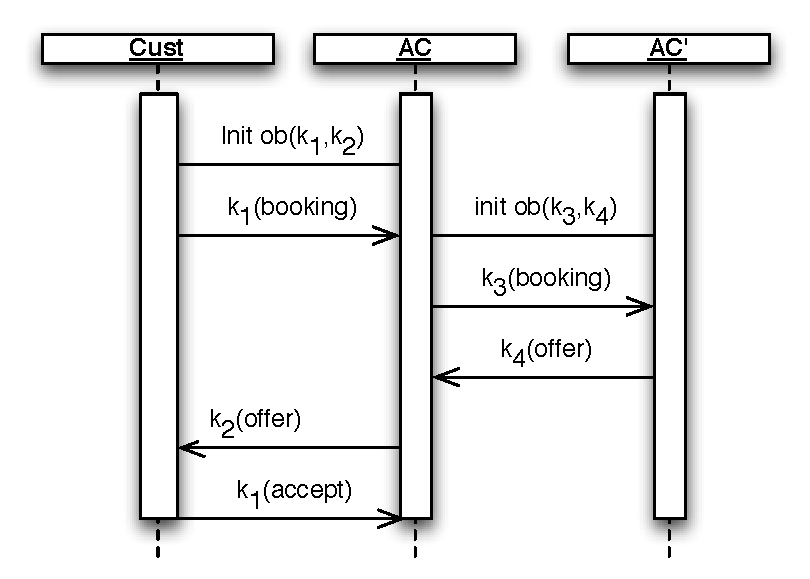
\includegraphics[width=1.00\textwidth]{LogicalProjection-introExample-welltyped}
       \caption{Interaction diagram (following classical session types)}
     \end{subfigure} \\
     \begin{subfigure}[b]{0.65\textwidth}
       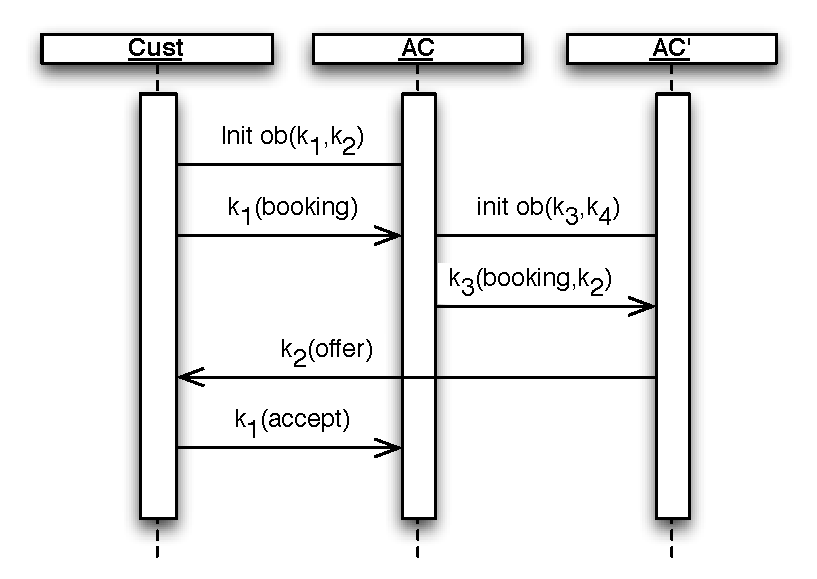
\includegraphics[width=1.00\textwidth]{LogicalProjection-introExample-delegation}
       \caption{Interaction diagram (session types with delegation)}
       \centering
     \end{subfigure} 
    \caption{Electronic booking example}
    \label{Logic4Struct:introduction::example}
\end{myfigure}



  A global specification focuses on the description of the
  interactions between participants $Cust, AC$ and $AC'$. For
  instance, $\init{\text{Cust}}{\text{AC}}{\text{ob}_{AC}}{k_1} $
  initiates an interaction between the Customer and the service
  $ob_{AC}$ located in the Airline company, labelled with a session
  identifier $k_1$. Similarly, the communication of the offer message
  between the Airline partner and the customer will be written as
  $\interact{\text{AC'}}{\text{Cust}}{k_2}{\text{offer}}{y}
  $. Choreographies $C_{OB-i}$ present possible specifications of 
  message exchanges in Figure
  \ref{Logic4Struct:introduction::example}, where  $C_{OB-1}$
  presents the alternative where messages travel back through AC,
  $C_{OB-2}$ the alternative creating a new session, and $C_{OB-3}$
  the alternative using session delegation.
  Notice that, in order for models like the ones described in $C_{OB-2}$
  and $C_{OB-3}$ to respect the causality and coherence relations
  between interactions present in the theory of
  session types, we need languages to
  be expressive enough to support further capabilities, like delegation \cite{honda1998lpa} and correlation sets
  \cite{lapadula7cows}. 

  \begin{align} \label{Logic4Struct:intro::example}
  C_{OB-1} = {} & \init{\text{Cust}}{\text{AC}}{\text{ob}_{AC}}{k_1,k_2} \pfx
  \interact{\text{Cust}}{\text{AC}}{k_1}{\text{booking}}{x_1} \pfx
  \notag \\
  & \init{\text{AC}}{\text{AC'}}{\text{ob}_{AC'}}{k_3,k_4} \pfx
  \interact{\text{AC}}{\text{AC'}}{k_3}{x_1}{y}  \pfx  \notag\\
  & \interact{\text{AC'}}{\text{AC}}{k_4}{\text{offer}}{x_2} \pfx
   \interact{\text{AC}}{\text{Cust}}{k_2}{x_2}{c}  \pfx \notag\\
   & \interact{\text{Cust}}{\text{AC}}{k_1}{\text{accept}}{z}
%    \\[0.5cm]
\end{align}
\begin{align}
  C_{OB-2} = {} & \init{\text{Cust}}{\text{AC}}{\text{ob}_{AC}}{k_1,k_2} \pfx
  \interact{\text{Cust}}{\text{AC}}{k_1}{\text{booking}}{x} \pfx
  \notag \\
  & \init{\text{AC}}{\text{AC'}}{\text{ob}_{AC'}}{k_3} \pfx
  \interact{\text{AC}}{\text{AC'}}{k_3}{k_2}{x'}  \pfx  \notag\\
  & \interact{\text{AC'}}{\text{Cust}}{k_2}{\text{offer}}{y} \pfx
  \interact{\text{Cust}}{\text{AC}}{k_1}{\text{accept}}{z} 
% \\[0.5cm]
\end{align}
\begin{align}
  C_{OB-3} = {} & \init{\text{Cust}}{\text{AC}}{\text{ob}_{AC}}{k_1,k_2} \pfx
  \interact{\text{Cust}}{\text{AC}}{k_1}{\text{booking}}{x_1} \pfx
  \notag \\
  & \init{\text{AC}}{\text{AC'}}{\text{ob}_{AC'}}{k_3,k_4} \pfx
  \interact{\text{AC}}{\text{AC'}}{k_3}{x_1}{y}  \pfx  \notag\\
  & \init{\text{AC'}}{\text{Cust}}{\text{ob}_{Cust}}{k_5,k_6} \pfx
  \interact{\text{AC'}}{\text{Cust}}{k_5}{\text{offer}}{c} \pfx \notag\\
  & \interact{\text{Cust}}{\text{AC}}{k_1}{\text{accept}}{z}
  \end{align}




  In the same way that a choreographical specification describes each
  of the interactions between participants, a logical characterisation
  of choreographies denotes formulae describing the evolution of such
  interactions. However, a logical characterisation gives more
  flexibility to the specification of interactions: One can forget
  about the addition of extraneous constructs of the language and
  define a simple policy about the behaviour of interactions. This
  policy can be described using logical
  specification over choreographies.  This logical
  specification describes \emph{only} the important parts of the message flow
  between participants. For instance, in the above presented
  specification, one can describe a property ensuring that, given a
  communication between the Customer and the Airline company with a
  booking message, there is an eventual response directed to the
  customer with an offer matching the same session identifier (in
  this case, not necessarily coming from the same participant the
  communication was initiated).

  {
    \begin{align} \label{Logic4Struct:intro::globalProperty}
      C_{OB-i} |= & \exists A,k_r  \pfx
      \actionF{\initF{Cust}{AC}{ob_{AC}(k_1,k_2)}} \pfx \actionF{\comF{Cust}{AC}{k_1
          (\text{booking}) }} \pfx \notag \\ 
      & \may \actionF{\comF{A}{Cust}{k_r (\text{offer}) }} 
    \end{align}
  }

  In a similar but orthogonal approach, the same specification in
  equation \ref{Logic4Struct:intro::example} can be seen as processes
  implementing each participant involved in the choreography. For
  instance, an interaction $\chor =
  \init{\text{Cust}}{\text{AC}}{\text{ob}_{AC}}{k_1,k_2} \pfx \chor'$
  describing session initiation can be decomposed to concurrent
  processes $\chor_{\text{Cust}} \pp \chor_{\text{AC}}$ implementing
  each side of the interaction:

  \begin{displaymath}
    \xymatrix{ 
      & \init{\text{Cust}}{\text{AC}}{\text{ob}_{AC}}{k_1,k_2} \pfx \chor'
      \ar@{->}[dr]^{\mathcal{\chor_{\text{AC}}}} \ar[dl]_{ \chor_{\text{Cust}}} &  \\ 
      \initOut{ob_{AC}}{k_1,k_2} \pfx \chor'_{\text{Cust}}  & \pp & \repInitIn{ob_{AC}}{k_1,k_2} \pfx \chor'_{\text{AC}}} 
\end{displaymath}

The full set of projections realising the choreography in equation
\ref{Logic4Struct:intro::example} might need to include participants Cust, AC and
AC', and will need to guarantee that the ordering of the messages
imposed in the global specification is still reflected in the
projections. The resulting behaviour can be seen below:

\begin{align} 
  \chor_{\text{Cust}} = {} & \initOut{ob_{AC}}{k_1,k_2} \pfx
  \send{k_1}{\text{booking}} \receive{k_2}{c}
  \send{k_1}{\text{accept}} \INACT \label{Logic4Struct:intro::endPoint::customer}\\
  \chor_{\text{AC}} ={} & \repInitIn{ob_{AC}}{k_1,k_2} \pfx \receive{k_1}{x_1}
  \initOut{ob_{AC'}}{k_3,k_4} \pfx \send{k_3}{x_1} \receive{k_4}{x_2}
  \send{k_2}{x_2} \receive{k_1}{z}\INACT \\
  \chor_{\text{AC'}} ={} & \repInitIn{ob_{AC'}}{k_3,k_4} \pfx\receive{k_3}{y}
  \send{k_4}{\text{offer}} \INACT \\
  \chor = {} & \chor_{\text{Cust}} \pp \chor_{\text{AC}} \pp \chor_{\text{AC'}}  \label{Logic4Struct:intro::endPoints}
\end{align}

A declarative vision of end points allows us to express properties
regarding each of the participants involved. For instance, we can
check that the end point representing the customer
respects a property stating that there is an eventual reply back after
having made a booking request. 
 Hence, the end point specification at Equation
\ref{Logic4Struct:intro::endPoint::customer} needs to satisfy the following formula:


\begin{align}
   \chor_{\text{Cust}} |=&
   \locatedActionF{Cust}{\asynchOutputF{k_1}{\text{booking}}} \pfx
   \may ~   \locatedActionF{Cust}{\asynchInputF{k_2}{x}} \pfx \endF
\end{align}

In the above,  $\locatedActionF{Cust}{\psi}$ denotes the execution of an action
$\psi$ by participant $Cust$.

An interesting point here is the relation we can evidence
between declarative specifications at global and local
viewpoints. In principle, a declarative model describing the behaviour
at the level of choreographies needs to be projected to formulae
describing the behaviour of their end-points.  Let $\phi_{OB}$ the formula
in Equation \ref{Logic4Struct:intro::globalProperty}, and its
decomposition into end-point formula described below:


\begin{align}
  [| \phi_{OB} |] = & \exists A, k_r. 
  (\locatedActionF{Cust}{\asynchServiceOutF{ob_{AC}}{k_1,k_2}} \pfx
  \locatedActionF{Cust}{\asynchOutputF{k_{1}}{\text{booking}}}  \\
   & \qquad \pfx ( \locatedActionF{Cust}{\asynchInputF{k_{r}}{\text{offer}}} \lor
   \may \locatedActionF{Cust}{\asynchInputF{k_{r}}{\text{offer}}} )) \notag
   \\
   & \pp (\locatedActionF{AC}{\asynchServiceInputF{ob_{AC}}{k_1,k_2}}
   \pfx   \locatedActionF{AC}{\asynchInputF{k_{1}}{\text{booking}}})
   \notag\\
   & \pp (\locatedActionF{A}{\asynchInputF{k_{r}}{\text{offer}}} \lor
   \may \locatedActionF{A}{\asynchInputF{k_{r}}{\text{offer}}})
\end{align}

The formula projected \emph{only} speaks about the projected behaviour
from the global specification, and allows for multiple implementations
of services to satisfy this specification. We will see later, that
although the translation seems intuitive, it is far from trivial: end
points can implement many threads at the same time, and those have to
be included in consideration on translations of the logical
formulae. Also, the projections considered should be
\emph{meaningful}, in the sense that they respect the theory of end
point projections. We show in further sections how this is accomplished.


\paragraph{Contributions}
Here we present a framework integrating imperative and declarative
views for structured communications. Building from previous research
in calculi for the specification of services, we
provide modal logic characterisations of the interactions occurring in
a system, both from a global point of view and from the point of view
of individual participants. The framework cope with two aims: exhibiting logical
guarantees about the presence of an interaction, and model generation
from logical specifications. In particular, we present two logical
languages for describing choreographies and orchestrations. First, \GL
is a logic describing possible interactions in a choreographical
language (the global calculus): the correspondence between
specifications in the calculus and the logic is tight, and one can go
either from the logical characterisation to the process algebraic
specification of a process, or prove that a choreographical
description respects a formula in \GL\!\!. Second, \LL is a logic
inspired by Hennessy-Milner with the aim of describing properties
about the interactions in a language of orchestrations (the end-point
calculus). The logic characterises typed bisimulation (pruning). As
the main result, we show that there is a correspondence between
imperative and declarative descriptions of the projections from
choreographies to its end-points. 


We pay special attention to the correspondence between imperative and
declarative descriptions for structured communications. The
correspondence presented here relies on the existence of meaningful
projections of choreographies to their corresponding end-points.  The
mapping is far from trivial, and needs to preserve causal relations
between messages and threads, namely connectedness, well-threadedness
and coherence. The theory describing mappings of this kind is normally
referred to as end-point-projections \cite{carbone7scc}, and is
achieved by equipping the global and the end-point calculus with
behavioural types.  Our main result in Theorem
\ref{Logic4Struct:theorem:lp:soundness} implies that for a well-typed
choreography $\chor$, and an associated choreographical formula
$\phi$, then 1) $\chor$ has a meaningful projection to end-point
behaviour, 2) $\phi$ has a logical projection to meaningful end-point
formulae, and 3) That satisfaction at the level of choreographies and
at the level of end-points coincide. This result relies on the use of
the type systems in \cite{carbone7scc}, which are included here for
completeness. A reader familiar with such type systems can easily skip
Section \ref{Logic4Struct-GlobalTypes},
Section\ref{Logic4Struct-EndPointTypes} and Section
\ref{Logic4Struct:sec:epp-types}.




\subsubsection{Overview of the document}

In Section \ref{Logic4Struct:sec:globalCalc} we give a summary of the
formal foundations of a calculus of choreographies, the so-called
global calculus. Its respective logic is presented in Section
\ref{Logic4Struct:sec:globalLogic}. We present undecidability results
for the logic on the global calculus in Section
\ref{Logic4Struct:sec:undecidability}. A proof
system relating the logical characterisation and the recursion-free
fragment of the global calculus shown in Section
\ref{Logic4Struct:sec:proofSys}. The semantics for the calculus of
end-points is presented in Section \ref{Logic4Struct:sec:epc}, a
logical characterisation of the end-point calculus is presented in
Section \ref{Logic4Struct:sec:localLogic}, as well as the main
contribution of this paper, namely the correspondence between the
end-point projection and the logical projection between global and
local formulae. Finally, concluding remarks are presented in Section
\ref{Logic4Struct:sec:conclusion}.


% When analysing service oriented systems, either we describe the system
% as the exchange of messages between different participants, or we
% consider the system as the composition of the local behaviours of each
% participant.  In this first view, known as \emph{choreography}, we
% consider the system as a whole, taking care only of the interfaces
% that participants use when interacting to the outside world. In the
% second view, known as \emph{orchestration}, we model the system as
% perceived by the eyes of each participant, sending and receiving
% messages but not knowing which other actors are present in a
% communication. A good illustration can be seen in the way a soccer
% match is planned: the coach has an overall view of the team, and
% organise how players will interact in each play (the role of a
% choreography) while each player performs his role by interacting with
% each of the members of his team by throwing/receiving passes. The way
% each player synchronise with other members of the team represents the
% role of an orchestration.
 
 
% The link between choreography and orchestration has been proposed in
% \cite{carbone7scc}. Here, choreography and orchestration constitute
% two interrelated approaches for modelling services. Two languages are
% proposed: A Global calculus to model choreographies and the End Point
% calculus to model orchestrations. Additionally, global and local
% specifications has already been shown operational correspondent under
% certain conditions, and one can generate an orchestrated model of a
% choreography by a mapping from the Global calculus to the End Point
% Calculus (something known as the \emph{End Point Projection (EPP)}).


% In this paper we aim at leveraging the trustworthiness level of a
% system by providing a clear methodology of specification and
% verification of structured communications.  Our goal is to provide
% service oriented systems with a \emph{logical characterisation}, both
% from the global perspective and from their end-point
% projections. Figure \ref{Logic4Struct:fig:serviceVerification} illustrates the
% approach for the specification and verification of service-oriented
% systems. We can analyse a choreography $C$ either by mapping a
% specification of global behaviour to a formula $\phi_C$ describing the
% interaction between participants, and from here generate $\bigcap_i [|
% \phi_i |]$, a set of formulas describing the local behaviour of each
% participant. Similarly, we can start from choreography $C$ and then
% use an end point projection to generate the parallel composition of
% the local behaviours of each participant involved in the communication;
% from here we can study their logical meaning as the set of formulas
% generated for each participant, closing the verification square.

% \begin{figure}[t]
% \begin{displaymath} 
% \xymatrix{ 
% C \ar@{<->}[r]^{\mathcal{GL}} \ar[d]_{EPP} &  \phi_C  \ar[d]^{?} \ar[dl]^{?} \\ 
% \prod_i[|P_i|] \ar@{<->}[r]_{\mathcal{LL}}  & \bigcap_{i}[|\phi_i |] } 
% \end{displaymath}
% \caption{Methodology for Service - Oriented Verification}
% \label{Logic4Struct:fig:serviceVerification}
% \end{figure}



% The end point projection between global and local specifications has
% been previously presented in \cite{carbone7scc}, and their operational
% correspondence property allow us to move from local to global
% perspectives and vice versa. Similarly, in a recent work
% \cite{Berger2008Completeness-an} a Hennessy-Milner logic for typed
% \mipi-calculi is introduced, providing the link between local
% specifications and logics.

% In this document we provide the link between choreographies and a
% logics (denoted as $\mathcal{GL}$ in Figure
% \ref{Logic4Struct:fig:serviceVerification}). Starting with an extension of
% Hennesy-Milner logic \cite{hennessy1980observing}, we provide a proof
% system that allows for property verification of choreographies. The
% logic is sound,
% %and complete
% in terms that a choreography will always reflect a logical state of
% the system.
% % , and a logical formula can always represent the state of a
% % choreography. Completeness also allows for checking of partial
% % specifications: if a property describing partial behaviour of the
% % system can be entailed by a choreography, then the whole system
% % would be able to fulfil such a property.
% Furthermore, a final step would conclude a methodology for
% verification of structured communications. The logic for
% choreographies should have a correspondent mapping to a logic to
% reason about end-point projections. \marginpar{fix this part!} This
% step, denoted by the transformation $LP$ between Global and Local
% formulas, is left as as further work of the current document.

% This paper is organised as follows: In section \ref{Logic4Struct:sec:globalCalc} we
% describe the global calculus as our reference language, with its
% syntax and operational semantics. Section \ref{Logic4Struct:sec:globalLogic}
% presents a logical language to express properties about
% choreographies, giving several examples of its use. Section
% \ref{Logic4Struct:sec:proofSys} presents the proof system and correctness results
% while in \ref{Logic4Struct:sec:conclusion} we discuss the future work.
% \marginpar{add part about GL and LL}

%%%%%%%%%%%%%%%%%%%%%%%%%%%%%%%%%%%%%%%%%%%%%%%%
% Introduction used in PLACES 2010                                                 %
%%%%%%%%%%%%%%%%%%%%%%%%%%%%%%%%%%%%%%%%%%%%%%%%

% \section{Introduction}
% Due to the continuous growth of technologies, software development is
% recently shifting its focus on communication, giving rise to various
% research efforts for proposing new methodologies dealing with higher
% levels of complexity. A new software paradigm, known as {\em
%   choreography}, has emerged with the intent to ease programming of
% communication-based protocols. Intuitively, a choreography is a
% description of the global flow of execution of a system where the
% software architect just describes which interactions \emph{might} take
% place. This idea differs from the standard approach where the
% communication primitives are given for each single entity
% separately. A good illustration can be seen in the way a soccer match
% is planned: the coach has an overall view of the team, and organises
% (a priori) how players will interact in each play (the role of a
% choreography); once in the field, each player performs his role by
% interacting with each of the members of his team by throwing/receiving
% passes. The way each player synchronise with other members of the team
% represents the role of an orchestration.
% %  A good illustration can be seen in the way a soccer match
% % is planned: the coach has an overall view of the team, and (a priori)
% % organises how players will interact in each play (the role of a
% % choreography). Instead, at run-time, each player performs his role by
% % interacting with each of the members of his team by throwing/receiving
% % passes according to what the coach has previously described.

 
 
% % The link between choreographies and orchestration has been proposed
% % in \cite{carbone7scc}. Here, choreographies and orchestration
% % constitute two interrelated approaches for modelling services. Two
% % languages are proposed: A Global calculus to model choreographies
% % and the End Point calculus to model orchestrations. Additionally,
% % global and local specifications has already been shown operational
% % correspondent under certain conditions, and one can generate an
% % orchestrated model of a choreography by a mapping from the Global
% % calculus to the End Point Calculus (something known as the \emph{End
% %   Point Projection (EPP)}).


% % In this work we focus on providing service oriented systems with a
% % \emph{logical characterisation} from a global perspective.  We can
% % analyse a choreography either by mapping a specification of global
% % behaviour to a formula describing the interaction between
% % participants.
% % Similarly, we can start from choreography and then use
% % an end point projection to generate the parallel composition of the
% % local behaviours of each participant involved in the communication;
% % from here we can study their logical meaning as the set of formulas
% % generated for each participant, closing the verification square.

% % \begin{figure}[ht]
% %   \begin{displaymath}
% % % \xymatrix{ 
% % % C \ar@{<->}[r]^{\mathcal{GL}} \ar[d]_{EPP} &  \phi_C  \ar[d]^{LP} \\ 
% % % \prod_i[|P_i|] \ar@{<->}[r]_{\mathcal{LL}}  & \bigcup_{i}[|\phi_i |] } 
% % \end{displaymath}
% % \caption{Methodology for Service - Oriented Verification}
% % \label{Logic4Struct:fig:serviceVerification}
% % \end{figure}



% % The end point projection between global and local specifications has
% % been previously presented in \cite{carbone7scc}, and their
% % operational correspondence property allow us to move from local to
% % global perspectives and vice versa. Similarly, in a recent work
% % \cite{Berger2008Completeness-an} a Hennessy-Milner logic for typed
% % \mipi-calculi is introduced, providing the link between local
% % specifications and logics.

% The work in \cite{CHY:dcm2006} formalises the notion of choreography
% in terms of a calculus, dubbed the {\em global calculus}, which
% pinpoints the basic features of the choreography paradigm. Although
% choreography provides a good abstraction of the system being designed
% allowing to {\em forget} about common problems that can arise when
% programming communication e.g. races over a channel, it can still have
% complex structures hence being often error prone. Additionally,
% choreography can be non-flexible in early design stages where the
% architect might be interested in designing only parts of a system as
% well as specifying only parts of a protocol (e.g. initial and final
% interactions). In this view, we believe that a logical approach can
% allow for more modularity in designing systems e.g. providing partial
% specification of a system using the choreography paradigm.

% In this document, we attempt to provide a link between choreography
% and logics. Starting with an extension of Hennessy-Milner logic
% \cite{hennessy1980observing}, we provide the syntax and the semantics
% of a logic for the global calculus as well as several examples
% pointing out the usefulness of the method. Moreover, we provide a
% proof system that allows for property verification of choreographies
% and show that it is
% sound. % Furthermore, a final step would conclude a
% % methodology for verification of structured communications. The logic
% % for choreographies should have a correspondent mapping to a logic to
% % reason about end-point projections. This step, denoted by the
% % transformation $LP$ between Global and Local formulas, is left as as
% % further work of the current document.
 
%%% Local Variables: 
%%% mode: latex
%%% TeX-master: "../Thesis"
%%% End: 


\section{The Global Calculus}\label{Logic4Struct:sec:globalCalc}

The Global Calculus (GC) \cite{CHY:dcm2006,carbone7scc} originates
from the Web Service Choreography Description Language (WS-CDL)
\cite{kavantzas2004web}, a description language for web services
developed by W3C. Terms in GC describe choreographies as interactions
between participants by means of message exchanges. The description of
such interactions is centred on the notion of \emph{session}, in
which two interacting parties first establish a private connection via
some public channel and then interact through it, possibly interleaved
with other sessions. More concretely, an interaction between two
parties starts by the creation of a fresh session identifier, that
later will be used as a private channel where meaningful interactions
take place. Each session is fresh and unique, so each communication
activity will be clearly separated from other interactions. In this
section, we provide an operational semantics for GC in terms of a
label transition system (LTS) \cite{plotkin81structural} describing
how global descriptions evolve, and the type discipline that describes
the structured sequence of message exchanges between participants from
\cite{carbone7scc}.

\subsection{Syntax}

Let $\chor, \chor', \ldots$ denote {\em terms} of the calculus, often
called {\em interactions} or {\em choreographies}; $A, B, C, \ldots$
range over {\em participants}; $k,k', \ldots$ are {\em linear
  channels}; $a,b,c,\ldots$ {\em shared channels}; $v,w,\ldots$
variables; $X,Y,\ldots$ process variables; $l,l_i,\ldots$ labels for
branching; and finally $e, e', \ldots$ over unspecified arithmetic and
other first-order expressions. We write $e@A$ to denote that the
expression $e$ is evaluated using the variable related to participant
$A$ in the store.

\begin{definition}\label{Logic4Struct:definition:globalCalc}
  The syntax of the global calculus \cite{CHY:dcm2006} is given by the
  following grammar:
  \begin{alignat}{3}
    \chor ::= \ & \phantom{{}\mid{}}
    &\ & \INACT                          \label{Logic4Struct:eq:Ginaction} \tag{inaction} \\
    &\mid && \init{A}{B}{a}{k}\pfx \chor \label{Logic4Struct:eq:Ginit} \tag{init} \\
    &\mid && \interact{A}{B}{k}{e}{y}\pfx\chor  \label{Logic4Struct:eq:Gcom} \tag{com} \\
    &\mid && \choice{A}{B}{k}{l}{\chor}   \label{Logic4Struct:eq:Gchoice} \tag{choice} \\
    &\mid && \chor_1 \pp \chor_2          \label{Logic4Struct:eq:Gpar} \tag{par} \\
    &\mid && \itn{e@A}{\chor_1}{\chor_2}  \label{Logic4Struct:eq:Gcond} \tag{cond}\\
    &\mid && X                            \label{Logic4Struct:eq:Grecvar} \tag{recvar} \\
    &\mid && \mu X\pfx C                  \label{Logic4Struct:eq:Grec} \tag{recursion}
  \end{alignat}
\end{definition}
\NI Intuitively, the term (\ref{Logic4Struct:eq:Ginaction}) denotes a
system where no interactions take place. (\ref{Logic4Struct:eq:Ginit})
denotes a session initiation by $A$ via $B$'s service channel $a$,
with a fresh session channel $k$ and continuation $\chor$. Note that
$k$ is bound in $\chor$.  (\ref{Logic4Struct:eq:Gcom}) denotes an
in-session communication of the evaluation (at $A$'s) of the
expression $e$ over a session channel $k$. In this case, $y$ does not
bind in $\chor$ (our semantics will treat $y$ as a variable in the
store of $B$).  (\ref{Logic4Struct:eq:Gchoice}) denotes a labelled
choice over session channel $k$ and set of labels $I$. In
(\ref{Logic4Struct:eq:Gpar}), $\chor_1 \pp \chor_2$ denotes the
parallel product between $\chor_1$ and $\chor_2$.
(\ref{Logic4Struct:eq:Gcond}) denotes the standard conditional
operator where $e@A$ indicates that the expression $e$ has to be
evaluated in the store of participant $A$.  In
(\ref{Logic4Struct:eq:Grec}), $\mu X\pfx\chor$ is the minimal fix
point operation for recursion, where the variable $X$ of
(\ref{Logic4Struct:eq:Grecvar}) is bound in $\chor$.  The free and
bound session channels, names, and term variables are defined in the
usual way, and are denoted as $fsc(\chor), bsc(\chor), fn(\chor),
fv(\chor)$.  

\begin{definition}[Structural congruence in GC]
GC is equipped with a standard structural
congruence $\equiv$, defined as the minimal congruence relation on
interactions $\chor$, such that $\equiv$ is a commutative monoid with
respect to $\pp$ and $\INACT$, it is closed under alpha equivalence
$\equiv_\alpha$ of terms, and it is closed under the recursion
unfolding, i.e., $ \mu X. \chor \equiv \chor \MSUBS{\mu X. \chor}{X}$.
\end{definition}

\begin{remark}[Differences with the approach in \cite{carbone7scc}]
  \label{Logic4Struct:remark::one}
  The syntax in Definition \ref{prelim:definition:globalCalc} presents
  a simplified version of the global calculus without restriction,
  summation and local assignments. In its original presentation, restriction is used only during session
  initiation. We capture the requirement of fresh identifiers by using
  the operational rules in Figure \ref{Logic4Struct:table:global:semantics}.
  Excluding the lack of local assignment, we argue that our version of
  GC is, to some extent, as expressive as the one originally reported
  in \cite{carbone7scc}.  In particular, the interaction
  process $\interact{A}{B}{k}{\mathsf{op},e}{y}$  as originally defined
  captures both selection and message passing which are instead
  disentangled in our case (mainly for reasons of clarity). The absence
  of $\mathsf{op}$ in the interaction process
  $\interact{A}{B}{k}{e}{y}$ can be easily encoded with the existing
  operators. In fact, $\interact{A}{B}{k}{\mathsf{op},e}{y} \pfx
  \chor'$ can be decomposed into $\choice{A}{B}{k}{op}{\chor'} \pfx
  \interact{A}{B}{k}{e}{y} \pfx \chor'$ with unary $I$ (although we
  lose atomicity).
\end{remark}



\subsection{Semantics}

We give the operational semantics in terms of configurations $(\sigma,
\chor)$, where $\sigma$ represents the state of the system and $\chor$
the choreography actually being executed. The state $\sigma$ contains
a set of variables labelled by participants. As described in the
previous subsection, a variable $x$ located at participant $A$ is
written as $x@A$.  The same variable name labelled with different
participant names denotes different variables (hence $\sigma(x@A$) and
$\sigma(x@B)$ may differ).  Formally, the operational semantics is
defined as a labelled transition system (LTS). A transition
$(\sigma,\chor) \action{\ell} (\sigma',\chor')$ says that a
choreography $\chor$ in a state $\sigma$ executes an action (or label)
$\ell$ and evolves into $\chor'$ with a new state $\sigma'$. Actions
are defined as
$\ell \in \{\initF{A}{B}{a(k)},\comF{A}{B}{k},\branchF{A}{B}{k}{l_i}\}$,
denoting initiation, in-session communication and branch selection,
respectively.  We write $(\sigma, \chor) \action{} (\sigma', \chor')$
when $\ell$ irrelevant, and $\action{}^*$ denotes the transitive
closure of $\action{}$. The transition relation $\action{}$ is defined
as the minimum relation on pairs state/interaction satisfying the
rules in Figure~\ref{Logic4Struct:table:global:semantics}.

\begin{myfigure}{t}
{\small
  \begin{align*}
&\myrule{    G-Init}
{ h \text{ fresh} } { ({\sigma,\init
        {A}{B}{a}{k}\pfx \chor}) \action{\initF{A}{B}{a(k)}}
      ({\sigma,\chor[h/k]}) }
\quad \myrule{    G-Struct}
{\chor\equiv \chor'' \quad
      ({\sigma,\chor}) \action{\ell} ({\sigma', \chor'}) \quad
      \chor'\equiv \chor'''} {({\sigma,\chor''}) \action{\ell}
      ({\sigma',\chor'''})}
   \\&
\myrule{    G-Choice}
{}
    {({\sigma,\choice{A}{B}{k}{l}{\chor}})
      \action{\branchF{A}{B}{k}{l_i}} ({\sigma,\chor_i})}
\quad 
\myrule{    G-Par}
{({\sigma,\chor_1}) \action{\ell}
      ({\sigma',\chor_1'})} {({\sigma,\chor_1\pp \chor_2})
      \action{\ell} ({\sigma',\chor_1'\pp \chor_2})}
    \\&
\myrule{    G-IfF}
{\sigma(e@A)\Downarrow \false \quad
      (\sigma, \chor_2) \action{\ell} (\sigma', \chor'_2)} { (\sigma,
      \itn{e@A}{\chor_1}{\chor_2}) \action{\ell}(\sigma',\chor'_2)}
\quad
\myrule{    G-IfT}
{\sigma(e@A)\Downarrow \true \quad
      (\sigma, \chor_1) \action{\ell} (\sigma', \chor'_1)} { (\sigma,
      \itn{e@A}{\chor_1}{\chor_2}) \action{\ell} (\sigma', \chor'_1) }
\end{align*} \vspace{-0.5cm}\begin{align*}
\myrule{    G-Com}
{\sigma(e@A)\Downarrow v} {
      ({\sigma,\interact{A}{B}{k}{e}{x}\pfx \chor})
      \action{\comF{A}{B}{k}} ({\sigma[x@B \mapsto v],\chor}) }
 \end{align*}
}
  \caption{Operational Semantics for the Global Calculus}
  \label{Logic4Struct:table:global:semantics}
\end{myfigure}

Intuitively, transition \Did{G-Init} describes the evolution of a
session initiation: after $A$ initiates a session with $B$ on service
channel $a$, $A$ and $B$ share the fresh channel $h$ locally.
% This will be denoted by a restriction of the session channel $k$
% over the continuation $C$, as denoted by $\new{k} C$.  The
% initiation channel $a$ will play an important role for typing and
% the end-point projection later.
\Did{G-Com} describes the main interaction rule of the calculus: the
expression $e$ is evaluated into $v$ in the $A$-portion of the state
$\sigma$ and then assigned to the variable $x$ located at $B$
resulting in the new state $\sigma [x@B \mapsto v]$. \Did{G-Choice}
chooses the evolution of a choreography resulting from a labelled
choice over a session key $k$. \Did{G-IfT} and \Did{G-IfF} show the
possible paths that a deterministic evolution of a choreography can
produce. \Did{G-Par} and \Did{G-Struct} behave as the standard rules
for parallel product and structural congruence, respectively.

\begin{remark}[Global Parallel]
  Parallel composition in the global calculus differs from the notion
  of parallel found in standard concurrency models based on
  input/output primitives \cite{milner:99:cmspc}. In the latter, a
  term $P_1\pp P_2$ may allow {\em interactions} between $P_1$ and
  $P_2$. However, in the global calculus, the parallel composition of
  two choreographies $\chor_1\pp \chor_2$ concerns two parts of the
  described system where {\em interactions} may occur in $\chor_1$ and
  $\chor_2$ but never across the parallel operator $\pp$. This is
  because an interaction $A\rightarrow B\ldots$ abstracts from the
  actual end-point behaviour, i.e., how $A$ sends and $B$ receives. In
  this model, dependencies between two choreographies can be expressed
  by using variables in the state $\sigma$.
\end{remark}

In its original presentation \cite{carbone7scc}, GC comes equipped
with a reduction semantics (presented for completeness in Figure
\ref{Logic4Struct:table:global:reduction-semantics}).
% unlike the one presented in Figure
% \ref{Logic4Struct:table:global:semantics}. 
Our LTS semantics has the advantage of
allowing us to observe the changes in the behaviour of the system by
presenting labels at each point of evolution. This  will
prove useful when relating to the logical characterisation in Section
\ref{Logic4Struct:sec:globalLogic}. 


\begin{myfigure}{t}
{\small
  \begin{align*}
&\myruleg{G-RInit}
{ h \text{ is fresh }  } { ({\sigma,\init {A}{B}{a}{k}\pfx \chor})  
          -->
      ({\sigma, \chor[h/k]}) }
\quad \myruleg{G-RStruct}
{\chor\equiv \chor'' \quad
      ({\sigma,\chor})  -->  ({\sigma', \chor'}) \quad
      \chor'\equiv \chor'''} {({\sigma,\chor''})  --> 
      ({\sigma',\chor'''})}
   \\[0.3cm]&
% \myruleg{G-RSum}
% { (\sigma, \chor_i) --> (\sigma', \chor' ) \quad i \in I}
%     {(\sigma, \sum_{i \in I} \chor_i)
%       --> ({\sigma',\chor'})}
% ~ 
\qquad \qquad \myruleg{G-RRec}
{ (\sigma, \chor [\rec X. \chor/\chor]) --> (\sigma', \chor' ) }
    {(\sigma, \rec X. \chor)
      --> ({\sigma',\chor'})}
\qquad 
\myruleg{G-RPar}
{({\sigma,\chor_1}) --> 
      ({\sigma',\chor_1'})} {({\sigma,\chor_1\pp \chor_2})
       -->  ({\sigma',\chor_1'\pp \chor_2})}
% ~
% \myruleg{G-RRes}
% {({\sigma,\chor}) --> ({\sigma',\chor'})}
%       {({\sigma, \new{k}\chor})
%        -->  ({\sigma', \new{k}\chor'})}
   \\[0.3cm]&
\myruleg{G-RIfT}
{\sigma(e@A)\Downarrow \true} { (\sigma,
      \itn{e@A}{\chor_1}{\chor_2})  --> (\sigma, \chor_1) }
\quad
\myruleg{G-RIfF}
{\sigma(e@A)\Downarrow \false } { (\sigma,
      \itn{e@A}{\chor_1}{\chor_2})  --> (\sigma,\chor_2)}
\end{align*} \vspace{-0.5cm}\begin{align*}
\myruleg{G-RCom}
{\sigma(e@A)\Downarrow v} {
      ({\sigma,\interact{A}{B}{k}{\mathsf{op},e}{x}\pfx \chor})
       -->  ({\sigma[x@B \mapsto v],\chor}) }
 \end{align*}}
  \caption{Reduction Semantics for the Global Calculus \cite{carbone7scc}}
  \label{Logic4Struct:table:global:reduction-semantics}
\end{myfigure}


% We conjecture that our proposed LTS semantics
% and the reduction semantics of the global calculus originally
% presented in \cite{carbone7scc} coincide (taking into account the
% considerations in Remark~\ref{Logic4Struct:remark::one}).




As it is expected, the labelled transition semantics above presented
and the reduction semantics of the global calculus originally
presented in \cite{carbone7scc}  coincide (taking into account the
considerations in Remark~\ref{Logic4Struct:remark::one}).

\begin{lemma} \label{struct:gc-opsem} if $\chor \equiv \chor''$ and
  $(\sigma,\chor) \action{\ell} (\sigma',\chor')$ then
  $(\sigma,\chor'') \action{\ell}(\sigma',\chor')$
  \begin{proof}
    It follows by induction on the structural congruence rules in
    $\equiv$ and second induction on the height of the derivation tree
    for $(\sigma,\chor) \action{\ell} (\sigma',\chor')$.
  \end{proof}
\end{lemma}

\begin{proposition}[Reduction and LTS semantics coincide in GC]
  Given $\chor, \chor'$ processes, $->$ the reduction relation between
  global calculus processes 
%  in \cite{carbone7scc}  (Included in
%   Appendix \ref{Logic4Struct:appendix:GlobalC-Rsemantics})
  and
  $\action{\ell}$ the labelled transition relation in Figure
  \ref{Logic4Struct:table:global:semantics}. We can say that:

\begin{description}
  \item [Soundness]: If $(\sigma, \chor) -> (\sigma', \chor')$, then
    $\exists \ell $ s.t. $ (\sigma, \chor) \action{\ell}^*
    (\sigma', \chor'')$ and $\chor' \equiv \chor''$.
  \item [Completeness]: For any $\ell$, if $(\sigma, \chor) \action{\ell} (\sigma',
    \chor')$ then $(\sigma, \chor) -> (\sigma',  \chor')$. 
\end{description}
\begin{proof} \hfill
\begin{description}

\item[On (Soundness):] \hfill \\ 
The proof proceeds by induction on the height of the derivation tree
for $(\sigma,\chor) -> (\sigma',\chor')$,
with a case analysis on the last applied rule. 
% The proof proceeds by induction on the length of
% derivation in $->$.
 \begin{description}
   \item[Case \Did{RG-Init}]: There must be the case that $\chor =
     \init{A}{B}{a}{k} \pfx \chor'$ and $(\sigma, \chor) ->(\sigma',
     %\new{k}
      \chor')$. One can easily show that for $\chor$ and $\ell=
     \initF{A}{B}{a(k)}$, $(\sigma, \chor)->(\sigma',\chor')$ which is
     structurally congruent to $%\new{k} 
     \chor'$ with fresh $k$ on
     $\chor'$.

   \item[Case \Did{RG-Comm}:] There must be the case that $\chor =
     \interact{A}{B}{k}{\mathsf{op}, e}{y} \pfx \chor'$ can be
     decomposed into $\choice{A}{B}{k}{op}{\chor'} \pfx
     \interact{A}{B}{k}{e}{y} \pfx \chor'$ (Remark \ref{Logic4Struct:remark::one}),
     so the reduction of $\chor$ will be given by $(\sigma, \chor) ->
     ^*(\sigma, \chor')$.

     By \Did{RG-Comm} one get that $(\sigma, \chor )->(\sigma [x@B |->
     v], \chor' )$, and one can easily show that for such a $\chor$,
     there is a transition $(\sigma, \chor) \action{\ell} ^* (\sigma,
     \chor')$, with $\ell$ variable depending on whether $\mathsf{op}$
     is used or not: 
     \begin{itemize}
       \item If $\mathsf{op} \not = \emptyset$, then we know that the behaviour
         maps to a deterministic choice, therefore $\ell =
         \branchF{A}{B}{k}{l}$ and $(\sigma,\chor)
         \action{\ell}(\sigma'', \chor'') $ $\action{\comF{A}{B}{k(x)}} (\sigma' [x@B |->
     v], \chor')$.
       \item If $\mathsf{op} = \emptyset$, then we know that the behaviour
         maps to message passing, therefore $\ell =
         \comF{A}{B}{k(x)}$ and $(\sigma,\chor)
         \action{\branchF{A}{B}{k}{l}}(\sigma'', \chor'') $ $\action{\ell} (\sigma' [x@B |->
     v], \chor')$.
      \end{itemize}
    \item[Case \Did{RG-IfT}:] We can assume that for $\chor = \itn{
        e@A }{ \chor_1 }{ \chor_2 }$ then $\sigma |- e@A \Downarrow
      \true$ and $(\sigma,\chor) -> (\sigma',\chor_1)$, the converse
      case is symmetric.
      
        From the application of $\Did{G-IfT}$ along with the induction
        hypothesis $(\sigma,\chor_1)\action{\ell}(\sigma',\chor'_1)$
        we get that $ (\sigma,\itn{e@A}{\chor_1}{\chor_2}) \action{\ell}
        (\sigma',\chor'_1)$ which is what we had to show.
      
        
        
        \item[Case \Did{RG-Par} and \Did{RG-Rec}]: Follows directly
          by simple rule induction.
          
        \item[Case \Did{RG-Struct}:] Given $(\sigma, \chor'') ->
          (\sigma,\chor''')$ then we can assume that $\chor \equiv
          \chor''$ and $(\sigma,\chor) -> (\sigma',\chor') \land
          \chor' \equiv \chor'''$. We need to show that
          $(\sigma,\chor'') \action{\ell}^* (\sigma,\chor''')$. From
          Lemma \ref{struct:gc-opsem} and the inductive hypothesis
          $\chor \equiv \chor'' \land (\sigma,\chor)
          \action{\ell}^*(\sigma',\chor') \land \chor' \equiv \chor'''$
          then $(\sigma,\chor'') \action{\ell}^* (\sigma',\chor''')$.
 \end{description}


\item[On (Completeness):] \hfill \\
The proof proceeds by induction on the height of the derivation tree for $(\sigma,\chor) \action{\ell} (\sigma',\chor')$,
with a case analysis on the last applied rule. 
% The proof proceeds by
% %  rule induction on the
% %   lenght of the derivations in $\action{\ell}$.
% case analysis of the labels
% in $\ell$ over the transitions in $(\sigma,C) \action{\ell}
% (\sigma',C')$. 

\begin{description}
  \item[Case $\ell = \initF{A}{B}{a(k)}$:] We have that $(\sigma,
    \chor) \action{\ell} (\sigma', \chor')$ with $\chor =
    \init{A}{B}{a}{k} \pfx \chor'$. After the application of
    $\Did{RF-Init}$ we get that $(\sigma,\chor)->(\sigma,\chor''[h/k])$
    with fresh $h$, and $\chor''[h/k] \equiv \chor'$, hence we are
    done.
    \item[Case $\ell = \comF{A}{B}{k(x)}$:] We have that
      $(\sigma,\chor) ->(\sigma[x@B \mapsto v], \chor')$ with $\chor =
      \interact{A}{B}{k}{e}{x} \pfx \chor'$. After the application of
      $\Did{RG-Comm}$ with $\mathsf{op} = \emptyset$ we get that
      $(\sigma,\chor)->(\sigma[x@B \mapsto v], \chor')$.
     \item[Case $\ell = \branchF{A}{B}{k}{l}$:] We have that
       $(\sigma,\chor)\action{\ell}(\sigma,\chor_i)$ with $\chor =
       \choice{A}{B}{k}{l}{\chor}$. After the application of
       $\Did{RG-Comm}$ with $\mathsf{l_i}$ we get that $(\sigma,\chor)
       ->(\sigma[x@B \mapsto v], \chor_i)$ with $x$ an irrelevant
       variable in $B$ (extra and not used elsewhere).
\end{description}

\end{description}
\end{proof}
\end{proposition}


\begin{example}[Online Booking]\label{Logic4Struct:ex:onlinebooking}
  We consider the example presented in the introduction, i.e., a
  simplified version of the on-line booking scenario presented in
  \cite{LOP-places09}. Here, the customer (Cust) establishes a session
  with the airline company (AC) using service (on-line booking,
  shorted as ob) and creating session keys $k_1,k_2$. Once sessions
  are established, the customer will request the company about a
  flight offer with his booking data, along the session key $k_1$. The
  airline company will process the customer request and will send a
  reply back with an offer using the session key $k_2$. The customer
  will eventually accept the offer, sending back an acknowledgment to
  the airline company using $k_1$. The following specification in the
  global calculus represents the protocol:
  \begin{align} \label{Logic4Struct:example:syntax} \chor_{\mathsf{OB}} = {} &
    \init{\text{Cust}}{\text{AC}}{\text{ob}}{k_1,k_2} \pfx
    \interact{\text{Cust}}{\text{AC}}{k_1}{\text{booking}}{x} \pfx \tag{OB} \\
    & \interact{\text{AC}}{\text{Cust}}{k_2}{\text{offer}}{y} \pfx
    \interact{\text{Cust}}{\text{AC}}{k_1}{\text{accept}}{z} \pfx
    \INACT \notag \, .
  \end{align}
\end{example}


\subsection{Session Types for the Global Calculus}
\label{Logic4Struct-GlobalTypes}

The Global Calculus comes accompanied wth a type discipline that
ensures the proper control flow among interactions. It is built as a
generalisation of session types \cite{honda1998lpa} for global
interactions, first presented in \cite{carbone7scc}.  Here we
informally describe
their use through examples, and direct the reader  to their original presentation for
a more formal view. 

Session types in
GC are used to structure sequence of message exchanges in a session.
Their syntax is as follows:
\begin{align}\label{Logic4Struct:eq:sessiontypes}
  \theta =& ~~\mathtt{bool} ~|~ \mathtt{ int}  ~|~ \ldots  \notag\\
  \alpha = & ~~
  \uparrow(\theta).\alpha
  ~|~
  \downarrow(\theta).\alpha
  ~|~
  \&\{ l_i: \alpha_i\}_{i\in{I}}
  ~|~ \oplus\{ l_i: \alpha_i\}_{i\in{I}}  ~|~ \alpha_1 \pp \alpha_2 ~|~ \endT ~|~ \mu \mathbf{
    t }\pfx \alpha ~|~  \mathbf{ t }
\end{align}

Here, $\theta$ range over standard data types $\mathtt{bool, string, int,
  \dots}$ and $\alpha$ describe session types.  We describe the forms
of $\alpha$. 
% The first four types are associated with the various
% communication operations:
\begin{itemize}
\item $\downarrow(\theta).\alpha$ and $\uparrow(\theta).\alpha$ are
  the input and output types and describe the reception (resp.
  emission) of a message with data type $\theta$ followed by a
  continuation $\alpha$.
\item Similarly, $\&\{ l_i: \alpha_i\}_{i\in{I}}$ is the branching
  type while $\oplus\{ l_i: \alpha_i\}_{i\in{I}}$ is the selection
  type.
 \item The type $\alpha_1 \pp \alpha_2$ is a parallel composition of
   session types $\alpha_1$ and $\alpha_2$. 
\item The type $\endT$ indicates session termination and is often
  omitted.
\item $\mu \mathbf{t} \pfx \alpha$ indicates a recursive type with
  $\mathbf{t}$ as a type variable. $\mu \mathbf{t} \pfx \alpha$ binds
  the free occurrences of $\mathbf{t}$ in $\alpha$. We take an
  \emph{equi-recursive} view of types, not distinguishing between $\mu
  \mathbf{t} \pfx \alpha$ and its unfolding $\alpha [\mu \mathbf{t}
  \pfx \alpha / \mathbf{t}]$.
\end{itemize}

Typing judgments in GC have the form $\typerule{\typeEnv}{}{\chor \ccc
  \Delta}$, where $\typeEnv$ is a type environment describing
\emph{services},  and $\Delta$  the type environment describing 
\emph{sessions}. Typically, $\typeEnv$
contains a set of type assignments of the form $a@A: \alpha$, which
say that a service $a$ located at participant $A$ may be invoked and
run a session according to type $\alpha$. $\Delta$ contains type
assignments of the form $k[A,B]: \alpha$ which say that a session
channel $k$ identifies a session between participants $A$ and $B$ and
has session type $\alpha$ when seen from the viewpoint of
$A$. There is no particular reason why one has to choose a
  strict direction when considering interactions, and one may as well
  consider $k[A,B]: \alpha$ from the viewpoint of $B$. We return to
the specification (\ref{Logic4Struct:example:syntax}) in
Example~\ref{Logic4Struct:ex:onlinebooking}
  to see how some of the typing rules work.  One possible assignment
  for $\Delta$ is:

 \begin{equation*}
       k_1, k_2 [Cust, AC]: k_1 \downarrow
       \text{booking}(\mathtt{string}) \pfx k_2 \uparrow
       \text{offer}(\mathtt{int}) \pfx k_1 \downarrow \text{accept}(\mathtt{string}) \pfx \endT 
\end{equation*}

Describing that $k_1$ and $k_2$ are names corresponding to the same
session between participants $Cust$ and $AC$, and corresponds to the
session type $\alpha = k_1 \downarrow
       \text{booking}(\mathtt{string}) \pfx k_2 \uparrow
       \text{offer}(\mathtt{int}) \pfx k_1 \downarrow
       \text{accept}(\mathtt{string}) \pfx \endT $ when seeing it from the
       point of view of $Cust$.

%  \begin{equation*}
%    \text{ob}@\text{AC}:(k_1,k_2) \pfx k_1 \downarrow
%     \text{booking}(\mathtt{string}) \pfx k_2 \uparrow
%     \text{offer}(\mathtt{int}) \pfx k_1 \downarrow \text{accept}
%     (\mathtt{int}) \pfx \endT \, .
% \end{equation*}
% the service type of
%   the airline company at channel $ob$ can be described as:


We provide some examples of the typing rules for the GC.
The full set of
typing rules derived from the original work are attached in Appendix
\ref{Logic4Struct:appendix:global:typing}.
First, we comment the rule \Did{G-TInit}, which types the establishment of a
new session between two participants. 
\begin{align*}
\myrule{    G-TInit}
    { \typerule{\typeEnv, a@B : (\vec{k})\alpha  }{}{
        \chor  \ccc \Delta \cdot \vec{k}[B,A]: \alpha \quad A \neq B} } { \typerule{\typeEnv, a@B : (\vec{k})\alpha  }{}{
        \init{A}{B}{a}{\vec{k}}\pfx \chor  \ccc \Delta}}
\end{align*} 

Here, the typing rule dictates some requirements on the structure of
the choreography: first, the initialisation of a session between
participants in $\init{A}{B}{a}{\vec{k}}\pfx \chor$ requires that 
sessions names in $\vec{k}$ correspond to a session type in the
premise. Moreover, it checks that the service channel $a@B :
(\vec{k})\alpha$ is declared in the service typing $\typeEnv$.
The rule $\Did{G-TCom}$ describes communication between
participants: 

\begin{align*}
    \myrule{    G-TCom}
    { \typerule{\typeEnv  }{}{
        \chor   \ccc \Delta \cdot \vec{k} [A,B] :\alpha}
      \quad \typerule{\typeEnv}{}{e@A:\theta}
      \quad \typerule{\typeEnv}{}{x@B:\theta}
      \quad k \in \vec{k}
      \quad A \neq B 
    } { \typerule{\typeEnv  }{}{
        \interact{A}{B}{k}{e}{x} \pfx \chor \ccc \Delta \cdot
        \vec{k}[A,B]: k \uparrow \theta \pfx \alpha}}
\end{align*}

Here, the interaction $ \chor = \interact{A}{B}{k}{e}{x} \pfx \chor'$
will be 
typable with a session type $\Delta \cdot
        \vec{k}[A,B]: k \uparrow \theta \pfx \alpha $ provided that:
        1) The evaluation of the expression $e$ at $A$ and its
        recipient variable $x$ at $B$ correspond to the same value
        type, 2) the communication is performed between different
        participants $A$ and $B$, and 3) the continuation
        $\chor$ contains a session type  between $A$ and $B$ such
        that its session names in $\vec{k}$ contain $k$. In the
        conclusion, we use an output type $k \uparrow \theta \pfx
        \alpha$ describing the emission of value from the point of view
        of $A$. It is clear, that we could use a complementary rule to
        type the input of values from the point of view of $B$.





\begin{assumption}[Well-typedness]
Henceforth we only consider well-typed terms for the Global calculus,
unless otherwise specified.  
% We hereafter assume In the sequel, we only consider choreographies that satisfy the
%   typing discipline.
\end{assumption}



%%%%%%%%%%%%%%%%%%%%%%%%%%%%%%%%%%%%%%%%%%%%%%%%%%%%
%%% Local Variables: 
%%% mode: latex
%%% TeX-master: "../Thesis"
%%% End: 
%%%%%%%%%%%%%%%%%%%%%%%%%%%%%%%%%%%%%%%%%%%%%%%%%%%%

%%%%%%%%%%%%%%%%%%%%%%%%%%%%%%%%%%%%%%%%%%%%%%%%%%%%
%%% Local Variables: 
%%% mode: latex
%%% TeX-master: "../Thesis"
%%% End: 
%%%%%%%%%%%%%%%%%%%%%%%%%%%%%%%%%%%%%%%%%%%%%%%%%%%%


\section{\texorpdfstring{\GL}{GL}: A Logic for the Global Calculus}\label{Logic4Struct:sec:globalLogic}

In this section, we introduce a logic for choreography.  The logical language comprises
assertions for equality and value/name passing.

\subsection{Syntax}
\begin{myfigure}{t!} \vspace{0.5cm}
  \begin{minipage}{.5\textwidth}
    \begin{alignat}{3}
      \phi, \chi \ ::= \ & \phantom{{} \mid {}}
      & \ & \exists \var\pfx \phi \label{Logic4Struct:eq:exists} \tag{f-exists}\\
      & \mid && \phi \land \chi \label{Logic4Struct:eq:and} \tag{f-and} \\
      & \mid && \neg \phi \label{Logic4Struct:eq:neg} \tag{f-neg} \\
      & \mid && \langle\ell\rangle \phi \label{Logic4Struct:eq:action} \tag{f-action} \\
      & \mid && \endF \label{Logic4Struct:eq:termination} \tag{f-termination} \\
      & \mid && e_1@A = e_2@B \label{Logic4Struct:eq:equality} \tag{f-equality} \\
      & \mid && \phi \mid \chi \label{Logic4Struct:eq:parallel} \tag{f-parallel} \\
      & \mid && \may \phi \label{Logic4Struct:eq:may} \tag{f-may} % \\
      % & \mid && X \label{Logic4Struct:eq:recvar} \tag{f-recvar} \\
      % & \mid && \mu X\pfx \phi \label{Logic4Struct:eq:rec} \tag{f-rec} \\
      % & \mid && \true \label{Logic4Struct:eq:true} \tag{true} \\
      % & \mid && \forall x^\rho\pfx \phi \label{Logic4Struct:eq:forall} \tag{forall} \\
      % & \mid && \nextOp \phi \label{Logic4Struct:eq:next} \tag{next} \\
      % & \mid && (\nu x)\phi \label{Logic4Struct:eq:new} \tag{new} \\
    \end{alignat}
  \end{minipage}
  \hfill
  \begin{minipage}{.5\textwidth}
    \begin{alignat}{3}
      \ell \ ::= \ & \phantom{{}\mid{}}
      &\ & \initF A B {a(k)} \label{Logic4Struct:eq:init} \tag{l-init} \\
      & \mid && \comF ABk && \label{Logic4Struct:eq:com} \tag{l-com}\\
      & \mid && \branchF ABkl & \label{Logic4Struct:eq:branch} \tag{l-branch}
    \end{alignat}
  \end{minipage}
  \caption{\texorpdfstring{\GL}{GL}: Syntax of formulae}
  \label{Logic4Struct:table:ChoreographyLogic}
\end{myfigure}
The grammar of assertions is given in
Figure~\ref{Logic4Struct:table:ChoreographyLogic}.  Choreography
assertions (ranged over by $\phi, \phi', \chi, \dots$) give a logical
interpretation of the global calculus introduced in the previous
section.  The logic includes the standard FOL operators $\land$,
$\neg$, and $\exists$. In $\exists \var \pfx \phi$, the variable
$\var$ is meant to range over service and session channels,
participants, labels for branching and basic placeholders for
expressions.  Accordingly, it works as a binder in $\phi$.  In
addition to the standard operators, the operator
(\ref{Logic4Struct:eq:action}) represents the execution of a labelled
action $\ell$ followed by the assertion $\phi$. Those labels $\ell$
match the ones in the LTS of GC, i.e., they are
(\ref{Logic4Struct:eq:init}), (\ref{Logic4Struct:eq:com}), and
(\ref{Logic4Struct:eq:branch}).  The formula
(\ref{Logic4Struct:eq:termination}) represents the process
termination.  We also include an unspecified, but decidable,
(\ref{Logic4Struct:eq:equality}) operator on expressions as in
\cite{Berger2008Completeness-an}.  (\ref{Logic4Struct:eq:may}) denotes
the standard eventually operators from Linear Temporal Logic (LTL)
\cite{emerson1991temporal}. The spatial operator
(\ref{Logic4Struct:eq:parallel}) denotes composition of formulae:
because of the unique nature of parallel composition in
choreographies, we have used the symbol $\mid$ (as in separation logic
\cite{reynolds2002sll} and spatial logic \cite{caires2001spatial}) in
order to stress the fact that there is no interference between two
choreographies running in
parallel. % Finally, the last two operators (\ref{Logic4Struct:eq:recvar}) and
% (\ref{Logic4Struct:eq:rec}) encodes the recursion for formulae.
We assume defined on formulas the standard relation $\equiv_\alpha$ of
$\alpha$-conversion.
 We also assume defined as usual the set $fn(\phi)$ of free name
 variables in $\phi$. If $m$ is a name and $\phi$ is a formula then
$\phi[t/m]$ denotes the formula obtained by replacing of all free
occurrences of $t$ in $\phi$ by the name term $m$, (nondeterministically) renaming bound
variables as needed to avoid capturing names in $m$.



\begin{notation}[Existential quantification over action labels]
  In order to simplify the readability, we introduce the concept of
  existential quantification over action labels as a short-cut to mean
  the following:
  \begin{alignat*}{2}
    \exists \ell \pfx \langle \ell \rangle \phi \ \DEFEQ {} \
    &&& \exists A,B,a,k \pfx
    \langle \initF{A}{B}{a(k)} \rangle \pfx \phi \lor {} \\
    &&& \exists A,B,k \pfx
    \langle \comF{A}{B}{k} \rangle \pfx \phi \lor {} \\
    &&& \exists A,B,k,l \pfx
    \langle \branchF{A}{B}{k}{l} \rangle \pfx \phi \, .
  \end{alignat*}
\end{notation}

\begin{remark}[Derived Operators]
  We can get the full account of the logic by deriving the standard
  set of strong modalities from the above presented operators. In
  particular, we can encode the constant true ($\true$) and false
  ($\false$); and the next ($\nextOp \phi$) and the always operators
  ($[] \phi$) from LTL.
  \begin{alignat*}{3}
    \true & \DEFEQ (0@A = 0@A) &\qquad\qquad
    \false  & \DEFEQ (0@A = 1@A) &\qquad
    (e_1 \neq e_2) & \DEFEQ \neg (e_1 = e_2) \\
    \forall x \pfx \phi & \DEFEQ \neg \exists x  \pfx \lnot \phi &
    \phi \lor \chi & \DEFEQ \lnot ( \lnot \phi  \land \lnot \chi) &
    \phi => \chi & \DEFEQ \lnot \phi \lor \chi \\
    [] \phi & \DEFEQ \lnot <<>> \neg \phi &
    [\ell] \phi & \DEFEQ \neg \langle \ell \rangle \neg \phi &
    \nextOp \phi & \DEFEQ \exists \ell \pfx \langle \ell \rangle \phi \, . % \\
    % (\nu X(\vec{x})\pfx \phi ) & = \neg (\mu X\pfx \neg \phi )
  \end{alignat*}
\end{remark}

In the rest of this section, we illustrate the expressiveness of our
logic through a sequence of simple, yet illuminating examples, giving
an intuition of how the modalities introduced plus the existential
operator $\exists$ allow to express properties of choreographies.

\begin{example}[Availability, Service Usage and Coupling]
  The logic above allows to express that, given a service invoker
  (known as $A$ in this setting) requesting the service $a$, there
  exists another participant (called $B$ in the example) providing $a$
  with $A$ invoking it.  This can be formulated in \GL as follows:
  \begin{equation*}
    \exists B \pfx \langle \initF{A}{B}{a(k)}\rangle \true \, .
  \end{equation*}
  Assume now, that we want to ensure that services available are
  actually used. We can use the dual property for availability, i.e.,
  for a service provider $B$ offering $a$, there exists someone
  invoking $a$:
  \begin{equation*}
    \exists A \pfx \langle \initF{A}{B}{a(k)}\rangle \true \, .
  \end{equation*}
  Verifying that there is a service pairing two different participants
  in a choreography can be done by existentially quantifying over the
  shared channels used in an initiation action. A formula in \GL
  representing this can be the following one:
  \begin{equation*}
    \exists a \pfx \langle \initF{A}{B}{a(k)} \rangle \true \, .
  \end{equation*}
\end{example}
\begin{example}[Causality Analysis]
  The modal operators of the logic can be used to perform studies of
  the causal properties that our specified choreography can fulfil.
  For instance, we can specify that given an expression $e$ evaluated
  to true at participant $A$, there is an eventual firing of a
  choreography that satisfies property $\phi_1$, whilst $\phi_2$ will
  never be satisfied.  Such a property can be specified as follows:
  \begin{equation*}
    (e@A = \true) \land <<>> (\phi_1) \land [] \lnot \phi_2 \, .
  \end{equation*}
\end{example}
\begin{example}[Response Abstraction]

 An interesting aspect of our logic is that it allows for the
  declaration of partial specification properties regarding the
  interaction of the participants involved in a choreography. Take for
  instance the interaction diagram in Figure~\ref{Logic4Struct:fig:diagram}.  The
  participant $A$ invokes service $b$ at $B$'s and then $B$ invokes
  $D$'s service $d$.  At this point, $D$ can send the content of
  variable $x$ to $A$ in two different ways: either by using those
  originally established sessions or by invoking a new service at
  $A$'s. However, at the end of both computation paths, variable $z$
  (located at $A$'s) will contain the value of $x$. In the global
  calculus, this two optional behaviour can be modelled as follows:
  \begin{myfigure}{t}\vspace{1cm}
    \begin{center}
      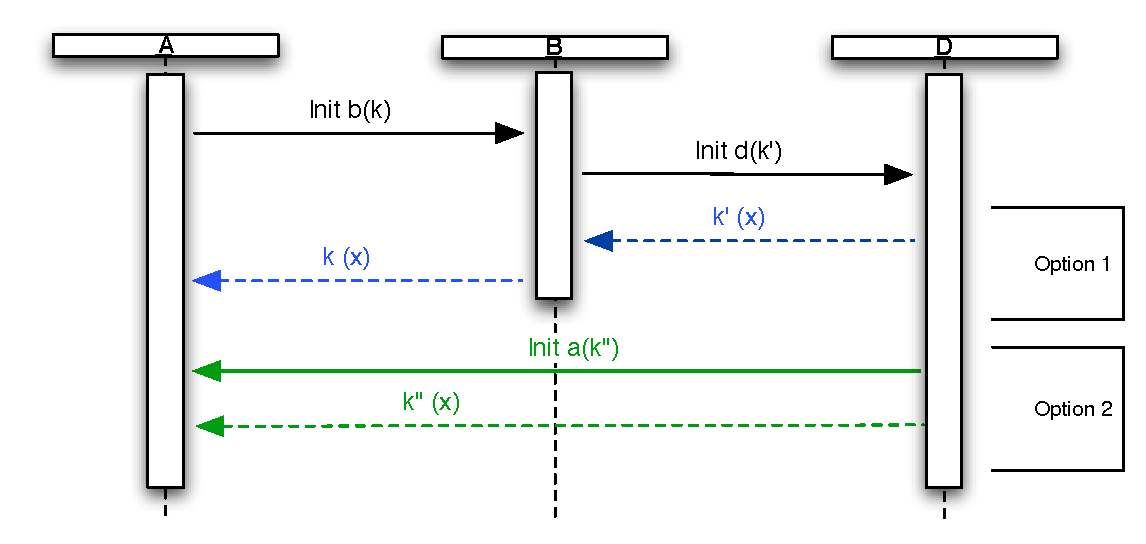
\includegraphics[width=\textwidth]{ServiceSynch}
    \end{center}
    \caption{Diagram of a partial specification.}
    \label{Logic4Struct:fig:diagram}
  \end{myfigure}

  \begin{align}
    C_1 & = \init{A}{B}{b}{k} \pfx \init{B}{D}{d}{k'} \pfx
    \interact{D}{B}{k'}{x}{y_B}\pfx\interact{B}{A}{k}{y_B}{z} \pfx \INACT 
    \label{Logic4Struct:eq:option1} \tag{Option 1} \\
    C_2 & = \init{A}{B}{b}{k} \pfx \init{B}{D}{d}{k'} \pfx
     \init{D}{A}{a}{k''}\pfx \interact{D}{A}{k''}{x}{z} \, \pfx \INACT \, .
     \label{Logic4Struct:eq:option2} \tag{Option 2}
  \end{align}
  We argue that, under the point of view of $A$, both options are
  sufficiently good if, after an initial interaction with $B$ is
  established, there is an eventual response that binds variable
  $z$. Such a property can be expressed by the \GL formula:
  \begin{equation*}
    \exists X,{k''}\pfx \langle\initF{A}{B}{a(k)} \rangle
    \may \Big(\langle \comF{X}{A}{k''}\rangle (z@A=x@D) \Big) \pfx \endT \, .
  \end{equation*}
  Notice that both the choreographies (\ref{Logic4Struct:eq:option1}) and
  (\ref{Logic4Struct:eq:option2}) \emph{satisfy} the partial specification
  above. This will be clear in Section~\ref{Logic4Struct:logic-assertions} where we
  introduce the semantics of logic.

  Also note that a third option for the protocol at hand is to use
  \emph{delegation} (the ability of communicating session keys to
  third participants not involved during session initiation). However,
  the current version of the global calculus does not feature such an
  operation and we leave it as future work.
\end{example}

\begin{example}[Connectedness]
  The work in \cite{carbone7scc} proposes a set of criteria for
  guaranteeing a safe end-point projection between global and local
  specifications (note that the choreography in the previous example
  does not respect such properties). Essentially, a valid global
  specification have to fulfil three different criteria, namely
  Connectedness, Well-threadedness and Coherence.  It is interesting
  to see that some of this criteria relate to global and local
  causality relations between the interactions in a choreography, and
  can be easily formalised as properties in the choreography logic
  here presented. Below, we consider the notion of connectedness and
  leave the other cases as future work. Connectedness dictates a
  global causality principle among interactions. If $A$ initiates any
  action (say sending messages, assignment, etc) as a result of a
  previous event (e.g. message reception), then such a preceding event
  should have taken place at $A$. In the following, let
  $\mathsf{Interact}(A,B)\phi$ be a predicate which is true whenever
  $\langle\ell\rangle\phi$ holds for some $\ell$ with an interaction
  from $A$ to $B$.  Connectedness can then be specified as follows:
  \begin{equation*}
    \forall A,B\pfx
    []
    \Big(
    \mathsf{Interact}(A,B)\true \Rightarrow {}  
    \exists C\pfx 
    \big(\mathsf{Interact}(A,B)\mathsf{Interact}(B,C)\true
    \lor 
    \mathsf{Interact}(A,B)\neg\exists\ell\langle\ell\rangle\true\big)
    \Big) \, . 
  \end{equation*}
%  {\bf Someone: to relate to Dimitris notion of connectedness.}
\end{example}

\subsection{Semantics}\label{Logic4Struct:logic-assertions}

\begin{myfigure}{t!}
  \centering
  \begin{displaymath}
    \begin{array}{lcl}
      \chor\ |=_\sigma \endF & \defSym & \chor \equiv \INACT 
      \\
      \chor\ |=_\sigma (e_1@A = e_2@B) & \defSym & \sigma(e_1@A)\Downarrow v\text{ and }\sigma(e_2@B)\Downarrow v 
      \\
      \chor\ |=_{\sigma}\actionF{ \ell}\phi&\defSym &  (\sigma,\chor)\action{\ell}(\sigma',\chor')\text{ and }\chor'|=_{\sigma'} \phi
      \\
      \chor\ |=_\sigma \phi\land\chi&\defSym &\chor|=_\sigma \phi \text{ and }\chor|=_\sigma \chi 
      \\
      \chor\ |=_\sigma \neg \phi & \defSym & \chor \not |=_\sigma \phi     
      \\
      \chor\ |=_\sigma \exists\var\pfx\phi & \defSym & \chor |=_\sigma \phi[w/\var]
      \text{ (for some appropriate $w$)}
      \\
      \chor\ |=_\sigma \may \phi & \defSym & (\sigma,\chor) \action{}^*(\sigma',\chor') \text{ and } \chor' |=_{\sigma'} \phi
      \\
      \chor\ |=_\sigma \phi \pp \chi & \defSym & \chor\ \equiv\ \chor_1\pp \chor_2 \text{ such that }
      \chor_1 |=_\sigma\phi \text{ and } \chor_2 |=_\sigma \chi
      % C\ |=_\sigma \nextOp \phi & \iff &
      % (\sigma, C) --> (\sigma', C')  \text{ and } C' |=_{\sigma'} \phi
      % \\
      % C\ |=_\sigma \new{k} \phi & \defSym & C \equiv \new{k} C' \text{ and }
      % C' |=_\sigma \phi 
      % \\
      % C\ |=_\sigma \phi \wand \chi & \iff & \forall C_1\pfx C \pp
      % C_1\text{well typed and } C_1 |=_\sigma \phi \text{ implies }C \pp C_1
      % |=_\sigma \chi\quad
      % \chor |=_\sigma \mu X\pfx \phi& \defSym & \chor = {\sf fix}\; \lambda \; f. \lambda \vec{v}. \phi[X / f][ \vec{x} / \vec{v}]
    \end{array}
  \end{displaymath}
  \caption{Assertions of the Choreography Logic}
  \label{Logic4Struct:table:global:assertions}
\end{myfigure}


We now give a formal meaning to the assertions introduced above with
respect to the semantics of the global calculus introduced in the
previous section. In particular, we introduce the notion of
satisfaction.  We write $\chor |=_\sigma \phi$ whenever a state
$\sigma$ and a choreography $\chor$ satisfy a \GL formula $\phi$.  The
relation $|=_\sigma$ is defined by the rules given in
Figure~\ref{Logic4Struct:table:global:assertions}.  In the
$\exists\var\pfx\phi$ case, $w$ should be an appropriate value
according to the type of $\var$, e.g., a participant if $\var$ is a
participant placeholder. Finally, $\sigma(e_1 @ A) \Downarrow$ denotes
the evaluation in the store $\sigma$ of a closed expression $e_1$ in
the participant $A$ with result $v$.

\begin{definition}[Satisfiability, Validity and Logical Equivalence in
  GL]\
  \begin{itemize}
  \item A formula $\phi$ is \emph{satisfiable} if there exists some
    configuration under which it is true, that is, $\chor |=_\sigma
    \phi$ for some $(\chor,\sigma)$.
  \item A formula $\phi$ is \emph{valid} if it is true in every
    configuration, that is, $\chor |=_\sigma \phi$ for every
    $(\chor, \sigma)$.
  \item A formula $\chi$ is a \emph{logical consequence} of a formula
    $\phi$ (or $\phi$ \emph{logically implies} $\chi$), denote with
    an abuse of notation as $\phi |= \chi$, if every configuration
    $(\chor,\sigma)$ that makes $\phi$ true also makes $\chi$ true.
  \item We say that a formula $\phi$ is \emph{logical equivalent} to
    a formula $\chi$, written $\phi \logicEquiv \chi$, if $\phi |= \chi$ iff
    $\chi |= \phi$.
    \item Given a set of formulae $\Phi$ and $\logicEquiv$, the
      equivalence class of $\phi \in \Phi$ is the subset of all
      elements in $\Phi$ such that are logically equivalent to $\phi$:
      \[
      [ \phi ] = \{ x \in \Phi | x \logicEquiv \phi \}
      \]
  \end{itemize}
\end{definition}

%\CommentHugo{ Define the list of formula equivalences for the
%Global Logic, otherwise it is difficult to know when two formulas
%represent the same.}
%
%\begin{proposition}%[Properties of $[ \phi ]$]
%  It holds that:
%     \begin{enumerate}
%       \item $\phi \in [ \phi ] $.
%        \item For any two equivalence classes $[ \phi ], [ \chi ]$, either
%          $[ \phi ]=[ \chi ]$ or $[ \phi ]$ and $[ \chi ]$ are
%          disjoint.
%          \item The set of all equivalence classes of $\Phi$ form a
%            partition of $\Phi$.
%            \item $\chi \logicEquiv \phi$ iff $[ \chi ] = [ \phi ]$.
%       \end{enumerate}
%
%\begin{proof}
%TBD
%\end{proof}
%\end{proposition}

%%% Local Variables: 
%%% mode: latex
%%% TeX-master: "../Thesis"
%%% End: 


\section{Undecidability of Global Logic} \label{Logic4Struct:sec:undecidability}
%
In this section we focus on the undecidability of the global logic for
the global calculus with recursion given in
Section~\ref{Logic4Struct:sec:globalCalc}.  In order to prove that the global logic
is undecidable, we use a reduction from the Post Correspondence
Problem (PCP)~\cite{Post:pcp} similarly to the one proposed in
\cite{ct:csl01}. The idea is to encode in the global calculus a
``program'' which simulates the construction of PCP.
%
We first give a formal definition of the PCP.  In the sequel, $\cdot$
denotes word concatenation.
%
\begin{definition}[PCP]
  Let $s,t,\ldots$ range over $\Sigma^*$ where $\Sigma = \{0, 1\}$ and
  let $\epsilon$ be the empty word.  An instance of PCP is a set of
  pairs of words $\{(s_1,t_1), \ldots, (s_n,t_n)\}$ over
  $\Sigma^*\times\Sigma^*$.  The Post Correspondence Problem is to
  find a sequence $i_0,i_1,\dots,i_k$ ($1 \leq i_j \leq n$ for all
  $0\leq j \leq k$) such that $s_{i_0}\cdot \ldots \cdot s_{i_k} =
  t_{i_0}\cdot \ldots \cdot t_{i_k}$.
\end{definition}

\NI Intuitively, PCP consists of finding some string in $\Sigma^*$
which can be obtained by the concatenation $s_{i_0}\cdot \ldots \cdot
s_{i_k}$ as well as by $t_{i_0}\cdot \ldots \cdot t_{i_k}$. This
problem is undecidable~\cite{Post:pcp}.
%
Our goal is to find a GC term that takes a random pair of words from
an instance of PCP and append them to an ``incremental pair'' of words
which encodes the current state of the sequences $s_{i_0}\cdot \ldots
\cdot s_{i_k}$ and $t_{i_0}\cdot \ldots \cdot t_{i_k}$.  Technically,
we need a choreography that assigns randomly a natural number in $\{1,
\dots, n\}$ to a variable $r$ in some participant $B$, and another
choreography that picks a pair of words from the PCP instance,
accordingly to value in the variable $r@B$, and then appends them to
the ``incremental pair'' of words in $A$.
Formally, % We suggest the following
% encoding:
\begin{definition}[Encoding of PCP]\label{Logic4Struct:def:PCPencoding}

  Let $A_1,\dots,A_n,A,B$ be participants and let $a,b$ be shared names for
  sessions, then define the two choreographies as shown below:
  \begin{align*}
    &
    \begin{array}{rcl}
      \textsf{Random}(A_1,\dots,A_n,B,a) &
      \DEFEQ &
      \phantom{{}\pp\ {}}\mu X \pfx
      \init{A_1}{B}{a}{k} \pfx
      \interact{A_1}{B}{k}{1}{r} \pfx X\\[1mm]
      &&
      \pp\ \mu X \pfx
      \init{A_2}{B}{a}{k} \pfx
      \interact{A_2}{B}{k}{2}{r} \pfx X\\[1mm]
      &&
      \pp\ \ldots\\[1mm]
      &&
      \pp\ \mu X \pfx
      \init{A_n}{B}{a}{k} \pfx
      \interact{A_n}{B}{k}{n}{r} \pfx X
      \end{array}
\end{align*}
\begin{align*}
    &
    \begin{array}{rcl}
      \textsf{Append}(A,B,b) &
      \DEFEQ &
      \mu X\pfx
      \init{A}{B}{b}{k} \pfx
      \interact{A}{B}{k}{str1}{tmp1} \pfx
      \interact{A}{B}{k}{str2}{tmp2} \pfx {} \\
      &
      &
      \mathbf{if}\ r@B = 1\ \mathbf{then} \\
      &
      &
      \quad
      \interact{B}{A}{k}{tmp1 \cdot s_1}{str1} \pfx
      \interact{B}{A}{k}{tmp2 \cdot t_1}{str2} \pfx X \\
      &
      &
      \mathbf{else}\ \mathbf{if}\ r@B = 2\ \mathbf{then} \\
      &
      &
      \quad
      \interact{B}{A}{k}{tmp1 \cdot s_2}{str1} \pfx
      \interact{B}{A}{k}{tmp2 \cdot t_2}{str2} \pfx X \\
      &
      &
      \mathbf{else} \ \mathbf{if}\ r@B = 3\ \mathbf{then} \\
      &
      &
      \qquad \vdots \\
      &
      &
      \mathbf{else} \ \mathbf{if}\ r@B = n\ \mathbf{then} \\
      &
      &
      \quad
      \interact{B}{A}{k}{tmp1 \cdot s_n}{str1} \pfx
      \interact{B}{A}{k}{tmp2 \cdot t_n}{str2} \pfx X \\
      &
      &
      \mathbf{else }\ X
    \end{array}
  \end{align*}
  We define the initial configuration $(\sigma,\chor)$ to be formed by
  the choreography and the state below:
  {\small
  \begin{align*}
    \chor & \DEFEQ
    \textsf{Random}(A_1,\dots,A_n,B,a) \pp  \textsf{Append}(A,B,b) \\
    \sigma & \DEFEQ
    [str1@A \mapsto \epsilon,\ str2@A \mapsto \epsilon,\
    tmp1@B \mapsto \epsilon,\ tmp2@B \mapsto \epsilon,\
    r@B \mapsto 1] \, .
  \end{align*}
  }
  For encoding the PCP existence question ($s_{i_0}\cdot \ldots \cdot
  s_{i_k} = t_{i_0}\cdot \ldots \cdot t_{i_k}$) we can encode it as a
  \GL formula:
  {\small
  \begin{equation*}
    \phi \DEFEQ
    <<>> \Big(
    (str1@A = str2@A) \land
    (str1@A \neq \epsilon) \land
    (str2@A \neq \epsilon)
    \Big) \, .
  \end{equation*}
  }
\end{definition}
\NI Above, each participant $A_i$ (with $i\in \{1,\dots,n\}$)
recursively opens a session with participant $B$ and writes in the
variable $r@B$ the value $i$. Moreover, the participant $B$ stores the
knowledge of all the word pairs $(s_i,t_i)$, while the participant $A$
takes randomly a word pair from $B$ and then append it to his
incremental pair of words: $(str1,str2)$.  Next, the formula $\phi$
states that there exists a computational path from the initial
configuration to a configuration which stores in $str1$ and $str2$ two
equal non-empty strings.

\begin{theorem}
  The global logic is undecidable for the global calculus with
  recursion.
\end{theorem}
\begin{proof} 
  (Sketch) The statement $\chor |=_\sigma \phi$ holds iff the encoded
  PCP has a solution.  Indeed, if the initial configuration
  $(\sigma,\chor)$ satisfies the formula $\phi$ then it means there
  exists a configuration $(\sigma',\chor')$ where $(str1@A = str2@A)
  \land (str1@A \neq \epsilon) \land (str2@A \neq \epsilon)$
  holds. Hence, there is a sequence of $i_0,\dots,i_k$ such that $str1
  = s_{i_0}\cdot \ldots \cdot s_{i_k} = t_{i_0}\cdot \ldots \cdot
  t_{i_k} = str2$, that is, the instance of PCP has a solution.
\end{proof}


\begin{remark}\label{Logic4Struct:remark:vars}
  The undecidability result presented in this section shows that the
  global calculus is considerably expressive, in spite of the fact
  that the choreography approach offers a simplification in the
  specification of concurrent communicating systems as argued in
  \cite{carbone7scc}. The encoding in
  Definition~\ref{Logic4Struct:def:PCPencoding} shows that allowing
  state variables (hence local variables that can be accessed by
  various threads) increases the expressive power of the
  language. Indeed, we could just look at GC as a simple concurrent
  language with a ``shared'' store where assignment to variables is
  just in-session communication. In this view, we conjecture that
  removing variables and focusing only on communication would make the
  logic decidable.
\end{remark}
% In the next sections, we discuss when and how to decide the global
% logic formulae on a sub-calculus of the global calculus.

%%% Local Variables: 
%%% mode: latex
%%% TeX-master: "main"
%%% End: 


\section{Proof System for \GL}\label{Logic4Struct:sec:proofSys}

% In a previous version of this
% article \cite{Carbone2010Towards-a-Modal}, we showed that \GL is
% undecidable for the global calculus with recursion, and
Here we  present a
model checking algorithm (in the form of a proof system) to decide
when a global logic formula is satisfied by a recursion-free
configuration of the global calculus. Indeed, similarly to
\cite{ct:csl01}, it turns out that the logic is decidable on the
recursion-free choreographies\footnote{As described in \cite{Carbone2010Towards-a-Modal}, removing recursion yields a
  decidability result in \GL}. We also prove the soundness and
completeness of the proposed proof system w.r.t.~the assertion
semantics.

In order to reason about judgments $\chor |=_\sigma \phi$, we propose
a proof (or inference) system for assertions of the form $\chor
|-_\sigma \phi$.  Intuitively, we want $\chor |-_\sigma \phi$ to be as
approximate as possible to $\chor |=_\sigma \phi$ (ideally, they
should be equivalent).  We write $\chor |-_\sigma \phi $ for the
provability judgement where $(\sigma,\chor)$ is a configuration and
$\phi$ is a formula.  

\begin{notation}
  We define the set of continuations, and the reachable set of
  configurations from an source configuration  $(\sigma, \chor)$, after an action
  $\ell$, as follows:
  \begin{align*}
    \textsf{Next}(\sigma,\chor,\ell) & \DEFEQ
    \{(\sigma',\chor') \mid (\sigma,\chor) \action{\ell} (\sigma',\chor')\}
    \\
    \textsf{Reachable}(\sigma,\chor) & \DEFEQ
    \{(\sigma',\chor') \mid (\sigma,\chor) \action{}^* (\sigma',\chor')\}
    \, .
  \end{align*}

Normalisation is required by the proof system to infer equality of
choreographies up to structural equi\-va\-len\-ce (Specially for the
$[ \cdot ] \pp [ \cdot ]$ operator).

  % We define $\textsf{Norm}(\chor)$ to be the normalisation of a
%   recursion-free choreography $\chor$:
 We define $\textsf{Norm}(\chor)$ to be a normalisation function from
  recursion-free choreographies into multisets of choreographies:
  \begin{align*}    
    &\textsf{Norm}(\interact{A}{B}{k}{e}{y}\pfx \chor) \DEFEQ
    [ \interact{A}{B}{k}{e}{y}\pfx \chor ]
    \\
    &\textsf{Norm}(\choice{A}{B}{k}{l}{\chor}) \DEFEQ
    [ \choice{A}{B}{k}{l}{\chor} ]
    \\
    &\textsf{Norm}(\init{A}{B}{a}{k}\pfx \chor) \DEFEQ
    [\init{A}{B}{a}{k}\pfx \chor]
    \\
    &\textsf{Norm}(\itn{e@A}{\chor_1}{\chor_2}) \DEFEQ
    [\itn{e@A}{\chor_1}{\chor_2}]    
    \\    
    &\textsf{Norm}(\INACT) \DEFEQ {[} \ {]}
    \\
    &\textsf{Norm}(\chor_1 \pp \chor_2) \DEFEQ [
    P_1,\dots,P_n,Q_1,\dots,Q_m ]
    \quad \text{if }
    \begin{array}{ll}
      \textsf{Norm}(\chor_1) = [P_1,\dots,P_n] & \text{and} \\
      \textsf{Norm}(\chor_2) = [Q_1,\dots,Q_m] & .
    \end{array}
  \end{align*}

\end{notation}

\begin{lemma}[Normalisation preserves structural equivalence]
  \label{Logic4Struct:lem:normalisation}
  Let $\chor$ be a recursion-free choreography and
  $\textsf{Norm}(\chor) = [P_1,\dots,P_n]$, then $\chor \equiv
  \prod_{i=1}^n P_i$.
\end{lemma}
\begin{proof}
  By induction on the structure of the choreography $\chor$.
   \begin{description}
   \item[Case $\chor = \INACT$:] We have $\textsf{Norm}(\INACT) = [\
     ]$, and $\prod_{i=1}^0 P_i = \INACT \equiv \INACT$.
   \item[Case $\chor = \chor_1 \pp \chor_2$:] We have that
     $\textsf{Norm}(\chor_1) = [P_1,\dots,P_n]$,
     $\textsf{Norm}(\chor_2) = [Q_1,\dots,Q_m]$, and $\prod_{i=1}^n P_i
     \equiv \chor_1$, $\prod_{j=1}^m Q_j \equiv \chor_2$ by induction
     hypothesis. Then, we can derive that $\prod_{i=1}^n P_i \pp
     \prod_{j=1}^m Q_j \equiv \chor_1 \pp \chor_2$.
   \item[All the other cases:] We have that
     $\textsf{Norm}(\chor) = [P_1]$, where $P_1 = \chor$, then
     $\prod_{i=1}^1 P_i \equiv \chor$. 
   \end{description}
\end{proof}

\begin{definition}[Entailment]
  We say that a choreography $\chor$ \emph{entails} a formula $\phi$
  under a state $\sigma$, written $\chor|-_\sigma \phi$, iff the
  assertion $\chor|-_\sigma \phi$ has a proof in the proof system
  given in Table~\ref{Logic4Struct:table:Global:proofSys}.
\end{definition}

\begin{table}
  \begin{gather*}
    \myruleg{P_{end}}{\textsf{Norm}(\chor) = [\ ]}
    {\typeruleE{\chor}{\sigma}{\endF}}
    ~
    \myruleg{P_{and}}{\typeruleE{\chor}{\sigma}{\phi} \quad
      \typeruleE{\chor}{\sigma}{\chi}} {\typeruleE{\chor}{\sigma}{\phi
        \land \chi}}
    ~
    \myruleg{P_{neg}}{ \chor \not |-_{\sigma} \phi}
    {\typeruleE{\chor}{\sigma}{\neg \phi}}
    ~
    \myruleg{P_{may}}{\exists (\sigma',\chor') \in
      \textsf{Reachable}(\sigma,\chor).\  \typeruleE{\chor'}{\sigma'}{\phi}}
    {\typeruleE{\chor}{\sigma}{\may \phi}}
    \\[1ex]
    \myruleg{P_{par}}{ \begin{matrix}[c]
        \textsf{Norm}(\chor) = [P_1,\dots,P_n] \\
        \exists I,J.\
        I\cup J = \{1,\dots,n\} \wedge
        I\cap J = \emptyset \wedge
        \typeruleE{\prod_{i\in I} P_i}{\sigma}{\phi_1} \wedge
        \typeruleE{\prod_{j\in J} P_j}{\sigma}{\phi_2} \end{matrix}
     }
    {\typeruleE{\chor}{\sigma}{ \phi_1 \pp \phi_2}}
  \\[1ex]
    \myruleg{P_{\exists}}
    {\exists w\in fn(\chor)\cup fn(\phi).\ 
      \typeruleE{\chor}{\sigma}{\phi[w/\var]}}
    {\typeruleE{\chor}{\sigma}{\exists \var \pfx \phi}}
    \qquad\qquad
    \myruleg{P_{exp}}{
      \sigma(e_1 @ A) \Downarrow v \quad \sigma(e_2 @ B) \Downarrow v}
    {\typeruleE{\chor}{\sigma}{ (e_1 @ A = e_2 @ B) }}
    \\[1ex]
    \myruleg{P_{action}}{\exists (\sigma',\chor') \in
      \textsf{Next}(\sigma,\chor,\ell).\  \typeruleE{\chor'}{\sigma'}{\phi}}
    {\typeruleE{\chor}{\sigma}{\langle\ell \rangle \phi}}
  \end{gather*}
  \caption{Proof system for the Global Calculus.}
  \label{Logic4Struct:table:Global:proofSys}
\end{table}

Let us now describe some of the inference rules of the proof system.
The rule $\mathsf{P_{end}}$ relates the inaction terms with the
termination formula. The rules $\mathsf{P_{and}}$ and
$\mathsf{P_{neg}}$ denote rules for conjunction and negation in
classical logic, respectively. The rule for parallel composition is
represented in $\mathsf{P_{par}}$; it does not indicate the behaviour
of a given choreography, but but provides information about the
structure of the process: $\mathsf{P_{par}}$ juxtaposes the behaviour
of two processes and combines their respective formulae by the use of
a separation operator. The next rule, $\mathsf{P_{action}}$ requires
that the process $P$ in the configuration $\sigma$ can perform an
action labelled $\ell$, so we must search for a continuations of
$(\sigma,\chor)$ after an action $\ell$ and find a configuration which
satisfies the rest of the formula, i.e., $\phi$.  Analogously,
$\mathsf{P_{may}}$ looks for a continuation in the reachable
configuration of $(\sigma,\chor)$ in order to satisfy $\phi$.  The rule
$\mathsf{P_\exists}$ says that in order to satisfy an $\exists t\pfx
\phi$, it is sufficient to find a value $w$ for $t$ in the free names
used by the choreography $\chor$ or in the free names used by the
formula $\phi$. Finally, the rule $\mathsf{P_{exp}}$ denotes
evaluation of expressions.

We now proceed to prove the soundness of the proof system with respect
to the semantics of assertions presented before.

\begin{lemma}[Structural congruence preserves satisfiability]
  \label{Logic4Struct:lemma:StructuralSatisfiability} If $\chor\equiv\chor'$ and
  $\chor|=_\sigma \phi$, then $\chor' |=_\sigma \phi$.
\end{lemma}
\begin{proof}
    It follows by induction on the structural congruence rules in
    $\equiv$ and second induction on the height of the derivation tree
    for   $\chor|=_\sigma \phi$.
    % It follows from simple case analysis over $\equiv$.
    We have the following cases:
   \begin{description}
   	\item[Case $P' \equiv P \pp \INACT$:]
		We have that  $P |=_\sigma \phi$ and $P \equiv P \pp \INACT $. By the definition of $|=$, 
		$P' |=_\sigma \phi \pp \psi$ iff $P' \equiv P \pp Q$, $P |=_\sigma \phi$ and $Q |=_\sigma \psi$. 
		Substituting $Q$ with $\INACT$, we have that $P' |=_\sigma \phi \pp \true$, that implies $P' |=_\sigma \phi$
	\item[Cases $P \pp Q \equiv Q \pp P$, $P \pp (Q \pp R) \equiv
          (P \pp Q) \pp R$ and $P \equiv_\alpha P'$:] They are
          straight-forward  as $\pp$ is commutative and associative in \GL and variable substitution does not affect provability.
%	\item[Case $P \equiv_\alpha P'$:]
   \end{description}
\end{proof}


\begin{theorem}[Soundness]\label{Logic4Struct:thm:soundness}
  For any configuration $(\sigma,\chor)$, where $\chor$ is
  recursion-free, and every formula $\phi$, if $\chor|-_\sigma \phi$
  then $\chor|=_\sigma \phi$.
\end{theorem}
\begin{proof}
The proof proceeds by induction on the height of the derivation tree
for $|-_\sigma$.
  \begin{description}
  \item[Case $\mathsf{P_{end}}$:] Straight consequence of
    Lemmas~\ref{Logic4Struct:lem:normalisation} and
    \ref{Logic4Struct:lemma:StructuralSatisfiability}, indeed $\chor \equiv \INACT$
    and $\chor |=_\sigma \endT$.
  \item[Case $\mathsf{P_{and}}$:] By induction hypothesis and
    conjunction.
  \item[Case $\mathsf{P_{neg}}$:] We have that $\chor|-_\sigma \lnot
    \phi$, so by $\mathsf{P_{neg}}$ we get $\chor \not |-_\sigma
    \phi$. By induction hypothesis we have that $\chor \not |=_\sigma
    \phi$, which is the necessary condition to deduce $\chor |=_\sigma
    \lnot \phi$.
  \item[Case $\mathsf{P_{par}}$:] We have that $\chor |-_\sigma
    \phi_1\pp \phi_2$, then $\textsf{Norm}(\chor) = [P_1,\dots,P_n]$,
    and there exist $I,J$ such that $I\cup J = \{1,\dots,n\}$, $I\cap J
    = \emptyset$, $\typeruleE{\prod_{i\in I} P_i}{\sigma}{\phi_1}$, and
    $\typeruleE{\prod_{j\in J} P_j}{\sigma}{\phi_2}$. By induction
    hypothesis we know that $\prod_{i\in I} P_i |=_\sigma \phi_1$ and
    $\prod_{j\in J} P_j |=_\sigma \phi_2$, then by
    Lemma~\ref{Logic4Struct:lem:normalisation} we have $\chor \equiv \prod_{i\in I}
    P_i \pp \prod_{j\in J} P_j$, hence it is immediate to prove that
    $\chor |=_\sigma \phi_1 \pp \phi_2$.
  \item[Case $\mathsf{P_{action}}$:] We have that $\chor |-_\sigma
    \langle \ell \rangle \phi$ and by $\mathsf{P_{action}}$ then
    $\chor' |-_{\sigma'} \phi$ and $(\sigma', \chor') \in
    \textsf{Next}(\sigma, \chor, \ell)$. From the induction hypothesis
    we have that $\chor' |=_{\sigma'} \phi$, then we have to show that
    $\chor |=_\sigma \actionF{\ell} \phi$. From the assertion
    semantics we know that $C |=_\sigma \actionF{\ell} \phi$ iff
    $(\sigma, \chor') \action{\ell} (\sigma', \chor')$ and $\chor'
    |=_{\sigma'} \phi$, which holds immediately by the selection of
    $(\sigma', \chor') \in \textsf{Next}(\sigma, \chor,\ell)$ and the
    induction hypothesis.
  \item[Case $\mathsf{P_{may}}$:] We have that $\chor |-_\sigma \may
    \phi$ and by $\mathsf{P_{may}}$ then $\chor' |-_{\sigma'} \phi$ and
    $(\sigma', \chor') \in \textsf{Reachable}(\sigma, \chor)$. From the
    induction hypothesis we have that $\chor' |=_{\sigma'} \phi$, then
    we have to show that $\chor |=_\sigma \may \phi$. From the
    assertion semantics we know that $C |=_\sigma \may \phi$ $ \iff
    (\sigma, \chor') \action{} ^* (\sigma', \chor')$ and $\chor'
    |=_{\sigma'} \phi$, which holds immediately by the selection of
    $(\sigma', \chor') \in \textsf{Reachable}(\sigma, \chor)$ and the
    induction hypothesis.
  \item[Case $\mathsf{P_{\exists}}$:] We have that $\chor |-_\sigma
    \exists t. \phi$ and by $\mathsf{P_{\exists}}$ we have that
    $\exists w \in fn(\chor) \cup fn(\phi)$ and $\chor |-_\sigma \phi
    [w/t]$. By induction hypothesis we know that $C |=_\sigma \phi
    [w/t]$ with appropriate $w \in fn(\chor) \cup fn(\phi)$, then
    $\chor |=_\sigma \exists t. \phi$ follows from the definition of
    the assertion semantics.
  \item[Case $\mathsf{P_{exp}}$:] It holds directly by checking if
    $\sigma(e_1@A) \Downarrow v$ and $\sigma(e_2@B) \Downarrow
    v$. 
  \end{description}
\end{proof}

The proof of completeness relies on a renaming lemma, that states that
logical properties are preserved over name permutations. These kind of
lemmas are standard among logical frameworks for process calculi
(e.g. \cite{cg:popl00,DBLP:conf/cmsb/MiculanB06}) and the general
  proof technique proceeds by induction on the syntax of formulae.


\begin{lemma}[Renaming preserves satisfiability]\label{Logic4Struct:lem:exists}
  Let $(\sigma,\chor)$ be a configuration with $\chor$ a recursion
  free choreography and a state $\sigma$. Let $\{n_1,\dots,n_k\}
  = fn(\chor) \cup fn(\phi)$. We can state that given  a formula $\phi$, $\chor |=_\sigma \exists t\pfx
  \phi$ if and only if $\exists m\in \{n_1,\dots,n_k\}$ such that $\chor
  |=_\sigma \phi[m/t]$.
\end{lemma}
\begin{proof}
  Both directions are proven via induction on the structure of
  $\phi$. We include some of the most relevant cases:
  \begin{description}
    \item[Case  $\phi = \phi_1 \pp \phi_2 $:] \hfill 
          \begin{description}
            \item[($=>$ side):] \hfill \\
              Given that $\chor |=_\sigma \exists t\pfx \phi_1 \pp
              \phi_2$ then $\chor \equiv \chor_1 \pp \chor_2$ and
              $\chor_1 |=_\sigma \exists t \pfx \phi_1 $ and $\chor_2
              |=_\sigma \exists t \pfx \phi_2$. We have to show that
              $\exists m \in fn(\chor) \cup fn(\phi_1 \pp \phi_2)$
              such that $\chor |=_\sigma (\phi_1 \pp \phi_2)[m/t]$.

              From the definition of $\phi$ and the induction
              hypothesis, we have that: 
              \begin{equation}
                \exists m \in fn(\chor_1) \cup
              fn(\phi_1) \text{ such that } \chor_1 |=_\sigma
              \phi_1[m/t]
              \end{equation} 
              Similarly, we know that 
              \begin{equation}
                \exists m \in
              fn(\chor_2) \cup fn(\phi_2) \text{ such that } \chor_2
              |=_\sigma \phi_2[m/t]
              \end{equation} 
              Note that, from $\chor \equiv
              \chor_1 \pp \chor_2$ we can infer that $fn(\chor) =
              fn(\chor_1) \cup fn(\chor_2).$, and from $\phi = \phi_1
              \pp \phi_2$. Then, $\exists m \in fn(\chor) \cup
              fn(\phi) $ such that $\chor  |=_\sigma (\phi_1 \pp
              \phi_2)[m/t]$.

              \item[($<=$ side):] \hfill \\
                Pick an $m$ such that $m \in fn(\chor) \cup
                fn(\phi_1 \pp \phi_2)$ and $\chor |=_\sigma (\phi_1
                \pp \phi_2)[m/t]$. we have to show that $\chor
                |=_\sigma \exists t\pfx (\phi_1 \pp \phi_2)$.

                From the assertion semantics, $\chor |=_\sigma
                (\phi_1 \pp \phi_2)[m/t]$ iff $\chor \equiv \chor_1
                \pp \chor_2$ and $\chor_1 |=_\sigma \phi_1[m/t]$ and
                $\chor_2 |= \phi_2 [m/t]$. 

                Now assume the induction hypothesis  $\chor_1 |=_\sigma
                \exists t \pfx \phi_1$ and $\chor_2 |= \exists t \pfx
                \phi_2$. Note  that $fn(\chor) \cup fn(\phi_1 \pp
                \phi_2) = fn(\chor_1) \cup fn(\chor_2) \cup fn(\phi_1
                \cup fn(\phi_2))$. Then, applying the induction hypothesis, we can
                conclude that $\chor |=_\sigma \exists t \pfx (\phi_1
                \pp \phi_2)$.
           \end{description}
      \item[Case $\phi = \actionF{\ell}\phi' $:] \hfill 
        \begin{description}
          \item[($=>$ side):] \hfill \\
            Given that $\chor |=_\sigma \exists t \pfx \actionF{\ell}
            \phi'$, then $\chor |=_\sigma \actionF{\ell}
            \phi'[m/t]$. Applying the definition in the assertion
            semantics, $(\sigma, \chor[m/t]) \action{\ell[m/t]}
            (\sigma',\chor'[m/t])$.  We have to show that $\exists m
            \in fn(\chor) \cup fn(\actionF{\ell}\phi')$ such that $\chor
            |=_\sigma \actionF{\ell} \phi'[m/t]$.

            We consider two cases for $m$: 1) $m \in fn(\chor') \cup
            fn(\phi') $, then after direct application of the
            induction hypothesis $C' |=_{\sigma'} \phi'[m/t]$ we get
            $\chor |=_\sigma \actionF{\ell} \phi'[m/t]$. 2)  In the
            case that $m \in (fn(\chor) \cup
            \fn(\actionF{\ell}\phi'))/(fn(\chor') \cup fn(\phi'))$.
            We know  that $fn(\chor') \subseteq \fn(\chor)$ and
            $\fn(\actionF{\ell} \phi') = fn(\phi')$. Then $m \in
            fn(\chor)/fn(\chor')$. From the application of  the  induction hypothesis
            $\chor'[m/t] |=_{\sigma'} \phi'[m/t]$ to  $\chor |=_\sigma \actionF{\ell} \phi'[m/t]$, we have that $\chor[m/t]
            |=_\sigma \actionF{\ell[m/t]}\phi'[m/t]$ implying 
            $\chor[m/t] |=_\sigma \actionF{\ell} \phi[m/t]$, 
            %, and given
%             $fn(\chor) = fn(\chor[m/t]) $
             then $\chor |=_\sigma
            \actionF{\ell} \phi'[m/t]$.

            \item[($<=$ side):] \hfill\\
              Pick $m \in fn(\chor) \cup fn(\actionF{\ell} \phi')$
              such that $\chor |=_\sigma \actionF{\ell}
              \phi'[m/t]$. We have to show that $\chor |=_\sigma
              \exists t \pfx \actionF{\ell} \phi'$.

              From the induction hypothesis, we have that $\chor'
              |=_{\sigma'} \phi'[m/t]$, which implies $\chor'
              |=_{\sigma'} \exists t \pfx \phi'$. Note that
              $fn(\chor') \cup fn(\phi') \subseteq fn(\chor) \cup
              fn(\actionF{\ell} \phi')$, then $\chor |=_\sigma \exists
              t \pfx \actionF{\ell} \phi$.
          \end{description}
        \item[Case $\phi = \exists t' \pfx \phi' $:] \hfill 
        \begin{description}
          \item[($=>$ side):] \hfill \\
            $\chor |=_\sigma \exists t. \exists t' \phi'$ then $\chor
            |=_\sigma (\exists t'. \phi')[m/t]$. We have to show that
            $\exists m \in fn(\chor) \cup fn(\exists t'. \phi')$ such
            that $\chor |=_\sigma (\exists t'. \phi')[m/t]$. From the
            the assertion semantics, we have that $\chor
            |=_\sigma \exists t \pfx \phi'[m/t] <=> \chor |=_\sigma \phi'[m'/t'][m/t]$. Select a name $m$, and use $\alpha-$conversion to
            ensure that $\sigma$ leaves unchanged all bound variables
            in the choreography $\chor$ and the formula $\phi'$.  Then $m \neq m'$ and
            $\chor |=_\sigma \phi[m'/t'][m/t]$. From the induction
            hypothesis we know that $m' \in fn(\chor) \cup fn(\exists
            t'. \phi')$ such that $\chor |=_\sigma \phi[m'/t']$. Given
            $fn(\exists t. \exists t' \phi') = fn(\exists t'. \phi')
            \cup t$, then $\chor |=_\sigma \phi'[m'/t'][m/t]$.
            \item[($<=$ side):] \hfill\\
              Pick a name $n \in fn(\chor) \cup fn(\exists x. \phi)$
              such that $\chor |=_\sigma \exists x . \phi'[m'/m]$. We use $\alpha-$conversion to
            ensure that $\sigma$ leaves unchanged all bound variables
            in the choreography $\chor$ and the formula $\phi'$.  We have to show that $\chor |=_\sigma \exists
              x. \exists m. \phi'$. After $\alpha$-renaming, we have to consider the possible
              selections of $n$.
              \begin{description}
                \item[($n\neq m' \land n\neq m$):] We have that $\chor
                  |=_\sigma \phi' [m'/m][n/x]$. Since $n\neq m'$ then
                  $\phi[m'/m][n/x] = \phi' [n/x][m'/m]$. Since $n\neq
                  m$ then $m' \not \in fn(\chor) \cup fn(\phi'[n/x])$
                  therefore $m' \in fn(\chor) \cup fn(\exists x. \phi' )$,
                  and  $\chor |=_\sigma \exists x. \exists m .
                  \phi'$.
                  \item[($n\neq m' \land n=m$):] We have that $\chor
                    |=_\sigma \phi'[m'/m][m/x]$. Since $n =m$ then
                    $\phi'[m'/m][m/x] = \phi'[m'/x]$. Then, $m' \in
                    fn(\chor) \cup fn(\exists m. \phi')$  and,
                    applying the induction hypothesis $\chor |=_\sigma \exists
                    m \pfx \phi'$ leads to  $\chor |=_\sigma \exists x. \exists m
                    \pfx \phi' \land x = m$.
%                     ..... $\exists x \pfx \exists m \pfx \phi'$. From $n \neq
%                     m'$ then $m' \in fn(\chor) \cup fn(\exists m. \phi')$
                \end{description}
          \end{description}
   \end{description}
%   (Sketch) By induction on the structure of $\phi$.  It is similar to
%   the proof of \cite[Lemma~5.3(3)]{cg:popl00}.
\end{proof}

\begin{theorem}[Completeness]\label{Logic4Struct:thm:completeness}
  For any configuration $(\sigma,\chor)$, where $\chor$ is
  recursion-free, and every formula $\phi$, if $\chor|=_\sigma \phi$
  then $\chor|-_\sigma \phi$.
\end{theorem}
\begin{proof}
  By rule induction on the derivation of $|=_\sigma$.
   \begin{description}
   \item[Case $\chor |=_\sigma \endT$:] We have that $\chor \equiv
     \INACT$ and hence $\textsf{Norm}(\chor) = [\ ]$ by
     Lemma~\ref{Logic4Struct:lem:normalisation}. Now, the thesis follows immediately
     from the application of $ \mathsf{P_{end}}$.
   \item[Case $\chor |=_\sigma (e_1 @ A = e_2 @ B)$:] It follows
     immediately by the application of $\mathsf{P_{exp}}$.
   \item[Case $\chor |=_\sigma \langle \ell \rangle \phi'$:] Take
     $(\sigma, \chor) \action{\ell} (\sigma',\chor')$ and $\chor'
     |=_{\sigma'} \phi' $, we have by induction hypothesis that
     $\typeruleE{\chor'}{\sigma'}{\phi'}$. Now, we have to show that
     $\chor |-_\sigma \langle \ell \rangle \phi'$.  By the fact that
     $(\sigma, \chor) \action{\ell} (\sigma',\chor')$, we have that
     $(\sigma', \chor')\in \textsf{Next}(\sigma,\chor,\ell)$, hence, we
     can apply rule $\mathsf{P}_{action}$ and we are done.
   \item[Case $\chor |=_\sigma \phi \land \chi$:] We have that $\chor
     |=_\sigma \phi$ and $\chor |=_\sigma \chi$. From the induction
     hypothesis we have that $\chor |-_\sigma \phi$ and $ \chor
     |-_\sigma \chi$. The application of $\mathsf{P_{and}}$ lead to
     $\chor |-_\sigma \phi \land \chi$ as desired.
   \item[Case $\chor |=_\sigma \lnot \phi$:] From the definition of the
     assertion semantics we have that $\chor |=_\sigma \lnot \phi $ iff
     $\chor \not |=_\sigma \phi$. We have to show that $\chor |-_\sigma
     \lnot \phi$. We proceed by contradiction. Take a $(\phi, \chor)$
     such that $\chor |-_\sigma \phi$, then from
     Theorem~\ref{Logic4Struct:thm:soundness} we have that $\chor |=_\sigma \phi$,
     which is a contradiction to $\chor |=_\sigma \lnot \phi$.
   \item[Case $\chor |=_\sigma \exists \var \pfx \phi$:] We have that
     $\chor |=_\sigma \exists t. \phi$ and by the definition in the
     assertion semantics we have that $\chor |=_\sigma \phi [w/t]$ for
     an appropriate $w$. By induction hypothesis we know that $\chor
     |-_\sigma \phi[w/t]$. Lemma~\ref{Logic4Struct:lem:exists} guarantees that there
     exists $w \in fn(\chor)\cup fn(\phi)$ in order to derive $\chor
     |-_\sigma \exists t. \phi$ from $\mathsf{P_{\exists}}$.
   \item[Case $\chor |=_\sigma <<>> \phi$:] Take $(\sigma, \chor)
     \action{}^* (\sigma',\chor')$ and $\chor' |=_{\sigma'} \phi'$, we
     have by induction hypothesis that
     $\typeruleE{\chor'}{\sigma'}{\phi'}$. Now, we have to show that
     $\chor |-_\sigma <<>> \phi'$.  By the fact that $(\sigma, \chor)
     \action{}^* (\sigma',\chor')$, we have that $(\sigma', \chor')\in
     \textsf{Reachable}(\sigma,\chor)$, hence, we can apply rule
     $\mathsf{P}_{may}$ and we are done.
   \item[Case $\chor |=_\sigma \phi \pp \chi$:] We have that $\chor
     \equiv \chor_1 \pp \chor_2$ and $\chor_1 |=_\sigma \phi \land
     \chor_2 |=_\sigma \chi$. From the induction hypothesis $\chor_1
     |-_\sigma \phi$ and $\chor_2 |-_\sigma \chi$. Now by
     Lemma~\ref{Logic4Struct:lem:normalisation} we have that $\chor_1 \equiv
     \prod_{i\in I} P_i$ and $\chor_2 \equiv \prod_{j\in J} P_j$ for
     some $I,J$. So, we can derive $\chor \equiv \prod_{i\in I} P_i \pp
     \prod_{j\in J} P_j$, and hence $\mathsf{P_{par}}$ leads to
     $\chor_1 \pp \chor_2 |-_\sigma \phi \pp \chi$. 
   \end{description} 
\end{proof}

\begin{theorem}[Termination]\label{Logic4Struct:thm:termination}
  For any configuration $(\sigma,\chor)$, where $\chor$ is
  recursion-free, and every formula $\phi$, proof-checking algorithm
  terminates.
\begin{proof}
  First, notice that all the functions \textsf{Norm}, \textsf{Next},
  and \textsf{Reachable} are total and computable. The proof is by
  induction over the structure of $\phi$.
   \begin{description}
   \item[Case $\phi = \endT$:] $\typeruleE{\chor}{\sigma}{\endT}$ iff
     $\textsf{Norm}(\chor) = [\ ]$.
   \item[Case $\phi = \phi_1 \land \phi_2$:] By conjunction and
     induction hypothesis on $\typeruleE{\chor}{\sigma}{\phi_1}$ and
     $\typeruleE{\chor}{\sigma}{\phi_2}$.
   \item[Case $\phi = \neg \phi'$:] $\typeruleE{\chor}{\sigma}{\phi}$
     iff $\typeruleE{\chor}{\sigma}{\phi'}$ does not hold. But by
     induction hypothesis we can construct a terminating proof or
     confutation for $\typeruleE{\chor}{\sigma}{\phi'}$. Hence the proof
     for $\typeruleE{\chor}{\sigma}{\phi}$ terminates as well.
   \item[Case $\phi = \phi_1 \pp \phi_2$:] Suppose
     $\textsf{Norm}(\chor) = [P_1,\dots,P_n]$. Notice that there exists
     a finite number of possible partitions of the index set
     $\{1,\dots,n\}$ as 
     $I \cup ,J$. Hence, for every $I \in ,J$ we can compute
     $\typeruleE{\prod_{i\in I} P_i}{\sigma}{\phi_1}$ and
     $\typeruleE{\prod_{j\in J} P_j}{\sigma}{\phi_2}$, which both
     terminate by induction hypothesis. By applying
     Lemma~\ref{Logic4Struct:lem:normalisation} we prove the thesis.
   \item[Case $\phi = \langle \ell \rangle \phi'$:] First, notice that
     the set $\textsf{Next}(\sigma,\chor,\ell)$ is finite, because the
     choreographies are finite, i.e., there are a finite number of
     actionable transition in a given configuration. For each
     configuration $(\sigma',\chor') \in
     \textsf{Next}(\sigma,\chor,\ell)$,
     $\typeruleE{\chor'}{\sigma'}{\phi'}$ terminates by induction
     hypothesis.
   \item[Case $\phi = <<>> \phi'$:] As before, notice that the set
     $\textsf{Reachable}(\sigma,\chor)$ is finite, because the
     choreographies are finite, i.e., the choreographies are recursion
     free. For each configuration $(\sigma',\chor') \in
     \textsf{Reachable}(\sigma,\chor)$,
     $\typeruleE{\chor'}{\sigma'}{\phi'}$ terminates by induction
     hypothesis.
   \item[Case $\phi = \exists t\pfx \phi'$:] To prove existence is
     sufficient to check every derivation by substituting $t$ with a
     name $w\in fn(\chor)\cup fn(\phi)$. Notice that $fn(\chor) \cup
     fn(\phi)$ is finite, because both $\chor$ and $\phi$ are so. So,
     for every $w$, we can construct a terminating derivation for
     $\typeruleE{\chor}{\sigma}{\phi'[w/t]}$ by induction hypothesis.
   \item[Case $\phi = (e_1@A = e_@@B):$]
     $\typeruleE{\chor}{\sigma}{(e_1@A = e_@@B)}$ iff $e_1@A \Downarrow
     v$ and $e_@@B \Downarrow v$.  
   \end{description}
\end{proof}
\end{theorem}



% \section{Proof System}\label{Logic4Struct:sec:proofSys}
% %
% In this section we present a proof system for the global logic.  In
% order to reason about judgments $\chor |=_\sigma \phi$, we propose a
% proof (or inference) system for assertions of the form $\chor
% |-_\sigma \phi$. Intuitively, we want $\chor |-_\sigma \phi$ to be as
% approximate as possible to $\chor |=_\sigma \phi$ (ideally, they
% should be equivalent). We write $\chor |-_\sigma \phi $ for the
% provability judgement where $(\sigma,\chor)$ is a configuration and
% $\phi$ is a formula.

% \begin{definition}[Exhibition - Choreography]
%   We say that a choreography $\chor$ \emph{exhibits} a formula $\phi$
%   under an environment $\sigma$, written $\chor|-_\sigma \phi$, iff
%   the assertion $\chor|-_\sigma \phi$ has a proof in the proof system
%   given in Table~\ref{Logic4Struct:table:Global:proofSys}.
% \end{definition}
% %
% \begin{table}[t]
%   \begin{align*}
%     & \myruleg{P_{init}}{\typeruleE{\chor}{\sigma}{\phi}}
%     {\typeruleE{\init{A}{B}{a}{k} \pfx \chor} {\sigma}{\langle
%         \initF{A}{B}{a(k)}\rangle\phi}} \qquad
%     \myruleg{P_{and}}{\typeruleE{\chor}{\sigma}{\phi} \quad
%       \typeruleE{\chor}{\sigma}{\chi}} {\typeruleE{\chor}{\sigma}{\phi
%         \land \chi}}
%     \\[1mm]
%     & \myruleg{P_{sel}}{\typeruleE{\forall i\in I.\
%         \chor_i}{\sigma}{\phi_i}} {\typeruleE{
%         \choice{A}{B}{k}{l}{\chor}}{\sigma}{\bigwedge_{i\in I} \langle
%         \branchF{A}{B}{l_i}{k}\rangle \phi_i}} \qquad
%     \myruleg{P_{neg}}{ \chor \not |-_{\sigma} \phi}
%     {\typeruleE{\chor}{\sigma}{\neg \phi}}
%     \\[1mm]
%     & \myruleg{P_{com}}{\typeruleE{\chor}{\sigma}{\phi}}
%     {\typeruleE{\interact{A}{B}{k}{e}{y}\pfx \chor }
%       {\sigma}{\langle\comF{A}{B}{k}\rangle \phi}} \qquad
%     \myruleg{P_{par}}{\typeruleE{\chor_1}{\sigma}{\phi_1} \quad
%       \typeruleE{\chor_2}{\sigma}{\phi_2}} {\typeruleE{\chor_1 \pp
%         \chor_2}{\sigma}{ \phi_1 \pp \phi_2}}
%     \\[1mm]
%     & \myruleg{P_{end}}{} {\typeruleE{ \INACT }{\sigma}{\endF}} \quad
%     \myruleg{P_{may1}}{ \typeruleE{\chor}{\sigma}{\phi}}
%     {\typeruleE{\chor}{\sigma}{\may \phi}} \quad \myruleg{P_{may2}}{
%       \typeruleE{\chor}{\sigma}{\phi \lor \nextOp \may \phi}}
%     {\typeruleE{\chor}{\sigma}{\may \phi}} \quad \myruleg{P_{exp}}{
%       \sigma(e_1) \Downarrow v \quad \sigma(e_2) \Downarrow v}
%     {\typeruleE{\chor}{\sigma}{ (e_1 = e_2) }}
%     \\[1mm]
%     & \myruleg{P_{ifT}}{\sigma(e@A) \Downarrow \true \quad
%       \typeruleE{\chor_1}{\sigma}{\phi}} {\typeruleE{ \itn
%         {e@A}{\chor_1}{\chor_2} }{\sigma}{\phi}} \qquad
%     \myruleg{P_{ifF}}{\sigma(e@A) \Downarrow \false \quad
%       \typeruleE{\chor_2}{\sigma}{\phi}} {\typeruleE{ \itn
%         {e@A}{\chor_1}{\chor_2} }{\sigma}{\phi}}
%     \\[1mm]
%     & \myruleg{P_{\exists}}{\exists w\in fn(\chor) \cup \{k\}.\
%       \typeruleE{\chor}{\sigma}{\phi[w/\var]} ~\text{ $k$ fresh}}
%     {\typeruleE{\chor}{\sigma}{\exists \var \pfx \phi}} \qquad
%     \myruleg{P_{struct}}{\typeruleE{\chor}{\sigma}{\phi} \quad
%       \chor\equiv \chor'} {\typeruleE{\chor'}{\sigma}{\phi}}
%     % &
%     % \myruleg{P_{var}}{ \mathbf{-} } {\typeruleE{ X }{}{\phi}}
%     % \qquad
%     % \myruleg{P_{rec}}{\typeruleE{C\MSUBS{\mu X.C}{X}}{}{\phi} }
%     % {\typeruleE{ \mu X\pfx C }{}{ \phi }}
%  \end{align*}
%  \caption{Proof system for the Global Calculus.}
%  \label{Logic4Struct:table:Global:proofSys}
% \end{table}

% \marginpar{Change the description aside accordingly to the change done
%   to the proof system} Let us now describe some of the inference rules
% of the proof system.  Any configuration satisfies $\mathsf{P_{true}}$.
% %$\mathsf{P_{var}}$ is the standard rule for recursion variables.
% The rule $\mathsf{P_{sel}}$ can be explained as follows: suppose we
% are given a process $P = \choice{A}{B}{k}{l}{\chor}$, a set of branch
% labels $\{l_i \, | \, i \in I\} $ (determined by typing) and we are
% given a proof that each $\chor_i$ satisfies $\phi_i$, then we
% certainly have a proof saying that every derivation of $P$ should
% satisfy a guard $l_i$ followed by a formula $\phi_i$.  The initiation
% and interaction rule $\mathsf{P_{init}, P_{com}}$ behave similarly to
% $\mathsf{P_{sel}}$: given an initiation/communication process in $P$
% and a proof that its continuation satisfies the proof term $\phi$, we
% can derive a proof that $P$ will first exhibit an
% initiation/communication action followed by $\phi$. The conditional
% rule $\mathsf{P_{if}}$ is standard. The subsumption rule
% $\mathsf{P_{sub}}$ is the standard consequence rule as found in Hoare
% logic.
% % and the rule $\mathsf{P_{rec}}$ just indicates that the formula
% % $\phi$ satisfied by a recursion will be also satisfied by its
% % unfolding.

% The rules for parallel composition and hiding are represented in
% $\mathsf{P_{par}}$ and $\mathsf{P_{res}}$ respectively, and they do
% not indicate the behaviour of a given choreography, but hint
% information about the structure of the process: $\mathsf{P_{par}}$
% juxtaposes the behaviour of two processes and combines their
% respective formulae by the use of a separation operator;
% $\mathsf{P_{res}}$ hides a variable $x$ in a formula $\phi$: The
% intuition is that since $\new x \chor$ is a choreography $\chor$ with
% $x$ restricted, if $\chor$ proves $\phi$ and $x$ is a fresh variable
% then $\new x \chor$ should satisfy $\phi$ with hidden $x$.

% We now proceed to prove the soundness of the proof system with respect
% to the semantics of assertions presented before.

% % \begin{lemma}[Monotonicity] \label{Logic4Struct:lemma:monotonicity} If $C --> C'$
% %   and $C' |=_\sigma \phi'$, then $C |=_\sigma \phi$ and $\phi \supset \phi'$.
% % \end{lemma}
% % \begin{proof}
% %   We have to proceed by induction on the structure of $-->$. I have
% %   not checked the details, and probably a discussion on this would
% %   be good (I don't think monotonicity is a good name for this?)
% % \end{proof}


% \begin{lemma}[Structural congruence preserves validity]
%   \label{Logic4Struct:lemma:StructuralLogic} If $\chor\equiv\chor'$ and
%   $\chor|-_\sigma \phi$, then $\chor' |-_{\sigma'} \phi$ and $\sigma
%   \subseteq \sigma'$.
% \end{lemma}
% \begin{proof}
%   It follows trivially from the rule $\mathsf{P_{struct}}$.
% \end{proof}

% \marginpar{adapt the following proofs to the new proof system}
% \begin{theorem}[Soundness]\label{Logic4Struct:thm:soundness}
%   For any choreography $\chor$, if $\chor|-_\sigma \phi$ then
%   $\chor|=_\sigma \phi$.
% \end{theorem}
% \begin{proof}
%   It follows by induction on the derivation of $|-_\sigma$.
%   \begin{description}
%   \item {Case $\mathsf{P_{end}}$:} We have that $\chor= \INACT$, then
%     $\INACT |-_\sigma \endF$ and $\INACT |=_\sigma \endF$ immediately.
%   \item {Case $\mathsf{P_{init}}$:} We have that $\chor =
%     \init{A}{B}{a}{k} \pfx \chor'$ and for $\phi = \langle
%     \initF{A}{B}{a(k)} \rangle \phi'$, then $\chor |-_\sigma \phi$ and
%     $\chor' |-_\sigma \phi'$.  We know that $\chor
%     \action{\initF{A}{B}{a(k)}} \chor'$ and also that $\chor'|=_\sigma
%     \phi'$ by induction hypothesis.  Hence, $\chor|=_\sigma \langle
%     \initF{A}{B}{a(k)} \rangle \phi'$ follows directly by definition
%     of $|=$.
%   \item {Case $\mathsf{P_{com}}$:} Analogous to the $\mathsf{P_{init}}$ case.
%   \item {Case $\mathsf{P_{sel}}$:} We have that $\chor =
%     \choice{A}{B}{k}{l}{\chor'} $ and $\chor|-_\sigma \bigwedge_{i \in
%       I} \langle \branchF{A}{B}{l_i}{k} \rangle \phi $. Because of
%     $\mathsf{P_{sel}}$ we have that $\forall i \in I.\, \chor_i
%     |-_\sigma \phi_i$ and by induction hypothesis, $\forall i \in I.\,
%     \chor_i |=_\sigma \phi_i$.  By definition of the semantics of
%     $\langle \ell \rangle \phi$ and conjunction, then:
%     \begin{equation*}
%       \chor |=_\sigma \bigwedge_{i \in I} \langle \branchF{A}{B}{l_i}{k} \rangle
%       \phi_i \text{ iff } \bigwedge_{i \in I} (\chor
%       \action{\branchF{A}{B}{l_i}{k}} \chor' \land \chor' |=_\sigma \phi_i )
%     \end{equation*}

%     Take $\ell = \branchF{A}{B}{l_i}{k}$ for $i \in I$, then $\chor
%     |=_\sigma \bigwedge_{i \in I} \langle \ell \rangle \phi_i$ if
%     $\ell = \branchF{A}{B}{l_i}{k}$ (trivially true) and if
%     $\chor\equiv (\nu s)(\choice{A}{B}{k}{l}{\chor'} | \chor'')$ which
%     is equivalent to $\chor$ up-to substitution $[s/k]$. Moreover,
%     $\exists \chor' \text{ s.t. } \chor --> \chor' \text{ and } \chor'
%     |=_\sigma \phi_i $ holds by induction hypothesis, so we are done.


%   \item {Case $\mathsf{P_{ifT}, P_{ifF}}$:} We take only the proof for
%     $\mathsf{P_{ifT}}$, the other works similarly. We have that $\chor
%     = \itn{e}{\chor_1}{\chor_2}$, by induction hypothesis we have that
%     $\chor_1 |-_\sigma e => \phi$ and $\chor_2 |-_\sigma \lnot e =>
%     \phi$.  We have to show that $\chor |=_\sigma \nextOp \phi $.
%     Assume a $\sigma$ s.t. $\sigma |-_\sigma e @ A \Downarrow \true$
%     (The other case is symmetric), then we get by the use of
%     \Did{G-IfT} with $\sigma$ and $\chor$ that $( \sigma, \chor) -->
%     (\sigma, \chor_1)$. Additionally we have that:
%     \begin{align*}
%       \chor_1  & |-_\sigma e @ A \Downarrow \true => \phi \\
%       \chor_1 & |-_\sigma \false \lor \phi \\
%       \chor_1 & |-_\sigma \phi
%     \end{align*}
%     Then, $\chor_1 = \chor' $ in $\exists \chor'\pfx \chor' |=_\sigma
%     \phi \text{ s.t. } \chor --> \chor' $, so we are done.


%   \item {Case $\mathsf{P_{res}}$:} We have that $\chor = \new{x}
%     \chor' $ and by induction hypothesis we have that $\chor'
%     |=_\sigma \phi $. We have to show that $\chor |=_\sigma \new{x}
%     \phi$ from $\chor |-_{\sigma} \new{x} \phi$.  From
%     $\mathsf{P_{res}}$, we know that $\chor' |-_\sigma \phi$ with $k$
%     a fresh variable. By definition, $\chor\ |=_\sigma \new{x} \phi $
%     if $\chor \equiv \new{x} \chor' $ and $\chor' |=_\sigma \phi$, so
%     we are done.

 
%  %%%%%%%%%%%%%HL: Recursion -- Removed for the progress report %%%%%%%%%%%
% % 
%  % \item Case $\mathsf{P_{rec}}$. We have that $C = \mu X^A\pfx C' $
%  %   and assuming the inductive hypothesis we have that $X |-
%  %   \phi$. We have to show that $\mu X \pfx C |=_\sigma \phi $.

% %Now, consider the following chain of formulae:

% %    \begin{align*}
% %      \mu^0 X \pfx \phi & =  \true \\
% %      & \dots \\
% %      \mu^{n+1} X \pfx \phi & =  \phi[\mu^n X\pfx \phi / X]
% %      \end{align*}

% %      By induction over ordinal numbers and the induction hypothesis
% %      we obtain
% %      \begin{equation}
% %        \mu X \pfx C |-_\sigma (\mu^n X \pfx \phi)
% %        \end{equation}
% %        Which is immediately true for $n= 0 $ and if is true for $n=m$
% %        then applying the inductive hypothesis and structural
% %        congruence is also true for $n = m + 1$. We can generalise
% %        this for all ordinals in $n$, so

% %        \begin{equation}
% %          \mu X \pfx C |-_\sigma (\mu X. \phi)
% %          \end{equation}

%   \item {Case $\mathsf{P_{par}}$:} Immediate.
%     \qed
%   \end{description}


% \end{proof}

% %%%%%%%%%%%%%%%%%%%%%%%%%%%%%%%%%
% % Completeness 
% %%%%%%%%%%%%%%%%%%%%%%%%%%%%%%%%%
% The following lemmata are used to prove completeness:

% \begin{lemma}[Structural congruence preserves satisfiability]
%   If $C \equiv C '$ and $C |=_\sigma \phi$, then $C' |=_\sigma \phi$
% \end{lemma}
% \begin{proof}
%   Follows directly from Lemma~\ref{Logic4Struct:lemma:StructuralLogic} and
%   Theorem~\ref{Logic4Struct:thm:soundness}. \qed
% \end{proof}

% \begin{lemma}[Operational semantics preserves substitutions]
% If $C \action{\ell} C'$ then  $C [w/\var] \action{\ell[w/\var]}
% C'[w/\var]$ for all $\ell$ and appropriate $w$.
% \begin{proof}
%   Follows by rule induction over $\action{\ell}$. \qed
% \end{proof}
% \end{lemma}
% \begin{lemma}[Substitution lemma] \label{Logic4Struct:lemma-substitution}
% For any choreography C; if $C |=_\sigma \phi$ then $C |=_\sigma \phi
% [w/\var]$ for an appropriate $w$.
% \end{lemma}
% \begin{proof}
% Follows by induction on the satisfaction relation of $C |=_\sigma
% \phi$. 
% % (The cases are in my notebook, yet to put them on latex). 
% \qed
% \end{proof}


% \begin{theorem}[Completeness]
%   For any choreography $C$, if $C |=_\sigma \phi$ then $C |-_\sigma \phi$.
% \end{theorem}

% \begin{proof}
%   By rule induction on the derivation of $|=_\sigma$.


%   \begin{itemize}
%   \item $(C |=_\sigma \true)$. Follows immediately from the application of $ \mathsf{T_{sub}}$.

%   \item $(C |=_\sigma \langle \ell \rangle \phi ')$. Take $C \action{\ell} C'
%     \land C' |=_\sigma \phi' $, we have to show that $C |-_\sigma \langle \ell
%     \rangle \phi'$.

%     We proceed by case analysis of $\ell$. 

%     \begin{itemize}
%       \item Take $\ell = \initF{A}{B}{a}$, then we know that $C |=_\sigma \langle
%     \ell \rangle \phi$ iff $C \action{\initF{A}{B}{a(k)}} D$ and $D |=_\sigma
%     \new{k} \phi$. We can also infer that $C = \init{A}{B}{a}{k} \pfx
%     C'$ and, by the application of $\Did{G-{init}}$ we get that $C
%     \action{\ell} D$ with $D = \new{k} C'$. From the application of
%     $\mathsf{P_{res}}$ and the induction hypothesis $\new{k}C' |-_\sigma
%     \new{k} \phi$ we get that $C' |-_\sigma \phi$, which is the necessary
%     condition to apply $\mathsf{P_{init}}$ over $C$, so we are done.

%   \item Take $\ell = \comF{A}{B}{k}$.  Then we know that $C =
%     \interact{A}{B}{k}{e}{x} \pfx C'$ and $C \action{\ell} C'$. 
%     $C |=_\sigma \langle \ell \rangle \phi ' $ iff $C \action{\ell} C'$ and $C'
%     |=_\sigma \phi' $. We can apply the induction hypothesis $C' |-_\sigma \phi'$
%     along $\mathsf{P_{com}}$ to get $C =
%     \interact{A}{B}{k}{e}{x} \pfx C' |-_\sigma \langle \comF{A}{B}{k} \rangle
%     \phi'$, so we are done.

%     A similar reasoning also holds for the case where $\ell =
%     \branchF{A}{B}{l}{k}$.
% \end{itemize}
% %%%%%%%%%%%%%%%%%%%%%%%%%%%%%%%%%%%%%%%%%%%%%%%%%%%
% % \nextOp \phi is just a generalisation from \langle \ell \rangle \phi
% % with free \ell, therefore this case is excluded from the proof.
% %%%%%%%%%%%%%%%%%%%%%%%%%%%%%%%%%%%%%%%%%%%%%%%%%%%

%   \item $(C |=_\sigma \new{x} \phi')$. Take $C \equiv (\nu v) C'$ and $C' |=_\sigma
%     \phi' (x \mapsto v)$. By structural congruence we have that
%     $\new{u} C' \equiv_\alpha \new{x} C'$ with fresh $x$ on $C'$, then
%     we can apply $\mathsf{P_{res}}$ with the induction hypothesis $C'
%     |-_\sigma \phi'$ to get $\new{x} C' |-_\sigma \new{x} \phi'$ and we are done.

%   \item $(C |=_\sigma \phi \land \chi)$. Follows immediately from the
%     application of the induction hypothesis $C |-_\sigma \phi \land C |-_\sigma
%     \chi$ and $\mathsf{P_{and}}$.

%   \item $(C |=_\sigma \phi \pp \chi)$. Immediate given $C \equiv C_1 \pp C_2$
%     and the application of the induction hypothesis $C_1 |-_\sigma \phi \land
%     C_2 |-_\sigma \chi$ with $\mathsf{P_{par}}$.

%   \item $(C |=_\sigma <<>> \phi)$. Take $(\sigma, C) --> ^* (\sigma',
%     C') $ and $C' |=_{\sigma'} \phi$, we have to show that $C |-_\sigma
%     <<>> \phi$.  We can express $(\sigma, C) -->^* (\sigma', C')$ as a
%     finite sequence of transitions $(\sigma, C) -->^n (\sigma',
%     C')$. We proceed by induction on $n$. 

%     If $n=1$, then $(\sigma, C) -->^1 (\sigma', C')$ and then the same
%     cases for $(\sigma, C) \action{\ell} (\sigma', C')$ can be
%     applied, so the proof will consider the same cases as the one in
%     $(C |=_\sigma \langle \ell \rangle \phi)$. Because we know
%     $\langle \ell \rangle \phi => \may \phi$, then we know that $C
%     |=_\sigma \may \phi$ and we are done.

%     If $n > 1$, then we know that $(\sigma, C) -->^{n-1} (\sigma'',
%     C'') --> (\sigma', C')$. By Induction hypothesis, we know that
%     $C'' |=_{\sigma''} \may \phi$. We need to show that $C
%     |=_{\sigma} \may \phi$. From $(\sigma'', C'') --> (\sigma', C')$
%     with any $\ell$, we know that $C |=_{\sigma} \nextOp \may \phi$,
%     which is subsumed by $\may \phi$ and we are done.

%   \item $(C |=_\sigma e_1 = e_2)$. Follows immediately by the
%     application of $\mathsf{P_{exp}}$.

%   \item $(C |=_\sigma \exists \var \pfx \phi)$.
%     Take $C[w/\var] |=_\sigma \phi$ for some appropriate $w$. We want
%     to show that $C |-_\sigma \exists \var \pfx \phi$. 
%     From lemma \ref{Logic4Struct:Logic4Struct:lemma-substitution} we have that $C |=_\sigma \phi
%    [w/\var]$.
% %  \item $(C |=_\sigma \phi \wand \chi)$.

%   \item $(C |=_\sigma \lnot \phi)$. TBD.

%   \end{itemize} \qed
% \end{proof}




%%% Local Variables: 
%%% mode: latex
%%% TeX-master: "../Thesis"
%%% End: 

%Deleted for the moment
% \input{transform}

%\input{transform}

\section{A calculus for orchestrations: The End-point Calculus }
\label{Logic4Struct:sec:epc}

\subsection{Syntax}
The end-point calculus (EPC) \cite{carbone7scc} is the $\pi$-calculus
\cite{milner:99:cmspc} extended with sessions \cite{honda1998lpa} as
well as locations \cite{hennessy2007distributed} and store
\cite{DBLP:conf/fsttcs/CarboneNS04}.  Below, $P, Q, \ldots$ denote {\em processes}, $M,
N, \ldots$ {\em networks}.
%\begin{table}[ht!]
\[\label{Logic4Struct:endpointsyntaxlable}
\begin{array}{ll}
%\begin{align*}
\begin{array}{rllll}
  P ::=
  &\phantom{{}\mid\quad}  \repInitIn {a}{\VEC{k}}\pfx P & \text{(initin)} 
  &\mid \quad \initOut{a}{\VEC{k}}\pfx P                  & \text{(initout)}\\
  &\mid\quad \send{k}{e} P                    &\text{(send)} 
  &\mid\quad \receive{k}{x} P                &\text{(receive)}\\
  &\mid\quad \selection{k}{\mathsf{l}} P  &\text{(label selection)} 
  &\mid\quad \branching{k}{\sum_i \mathsf{l_i} \pfx P_i}  &\text{(label branching)}\\
%   &\mid \quad\inputBranch{s}{i}{op}{{y}}{P}           & \text{(branch)} \\ 
%   &\mid\quad\outputP{s}{op}{{e}}\pfx P                & \text{(out)}\\
%  &\mid \quad x:=e\pfx P                                 & \text{(assign)} 
  &\mid \quad P_1\oplus P_2                              & \text{(plus)}    
  &\mid\quad  P_1\pp P_2                                 &
  \text{(par)}\\  
  &\mid \quad \rec X\pfx P                              & \text{(rec)}   
  &\mid\quad  X                                         & \text{(recvar)}\\
 &\mid\quad\itn{e}{P_1}{P_2}                     & \text{(cond)} 
%   &\mid \quad \new s P                                  & \text{(new)}     
  &\mid\quad  \INACT                                    & \text{(inact)}\\
\end{array}
\\\\ 

\begin{array}{rll}
  N
  ::=
  &\phantom{{}\mid\quad}   \pr AP\sigma
  &\text{(participant)}\\
  &\mid\quad  N_1\pp N_2 &\text{(parnet)}\\
%   &\mid \quad \new s N  & \text{(newnet)}    \\
  &\mid\quad  \INACTNW  &\text{(inactnet)}
\end{array}
\end{array}
\]
% \caption{End Point Calculus: Syntax }
% \end{table}
%\end{align*}


(initin) and (initout) are dual operations for describing session
initiation: $\repInitIn{a}{\VEC{k}} \pfx P$ denotes a process
offering a replicated (available in many copies) service $a$ with
session channels $\VEC{k}$ while $\initOut{a}{\VEC{k}} \pfx P$ denotes a
process requesting a service $a$ with session channels $\VEC{k}$. In
both cases, $P$ is the continuation. The next two processes denote
standard in-session communications (where $y_i$ in the first
construct, the branching input, is not bound in $P_i$, and $\{l_i\}$
should be pairwise distinct). 
%Next, $x := e \pfx P$ assigns the value
%of $e$ to $x$ in the store then continues as $P$.  
The term $\Did{plus}$
denotes internal choice. The rest is standard. Networks are parallel
composition of participants, where a participant has the shape $\pr
AP\sigma$, with $A$ being the name of the participant, $P$ its
behaviour, and $\sigma$ its local state, now interpreted as a local
function from variables to values. We often omit $\sigma$ when
irrelevant. The free session channels, free term variables and service
channels are defined as usual over processes and networks and,
similarly to the global calculus, are denoted by $fsc(P/N), fv(P/N)$ and
$channels(P/N)$ respectively. The syntax here presented differs from
its original presentation in the absence of the local assignments 
and restriction of networks and processes.

\subsection{Semantics}

Similarly to the Global Calculus, the EPC is equipped with a
structural congruence relation over networks and thread processes.
\begin{definition}[Structural Congruence in EPC]
The structural congruence relation $\equiv$ in EPC is the least
congruence on processes and networks such that $(\LITEQ, \INACT,
\oplus)$, 
% $(\LITEQ, \INACT, +)$, 
$(\LITEQ, \INACT, \pp)$ and $(\LITEQ,
\epsilon, \pp)$
% , $(\pp,\INACTNW)$ 
are commutative monoids and such
that 
% $ a) \new{s}\INACT \LITEQ \INACT$, 
% $ b) \new{s_1}\new{s_2}P
% \LITEQ \new{s_2}\new{s_1}P$, 
% $ c) \new{s}P\pp Q \LITEQ \new{s}(P\pp Q)
% ~(\text{for }s\not\in\fsc{Q})$, 
% $ d) \pr{A}{P}{\sigma} \LITEQ
% \pr{A}{Q}{\sigma} ~ (\text{for }P \LITEQ Q)$, 
% $ e)\pr{A}{\new{s}P}{\sigma} \LITEQ \new{s}(\pr{A}{P}{\sigma})$, 
% $ f)\new{s_1}\new{s_2}M \LITEQ \new{s_2}{\new{s_1}}M$, 
% $ g)\new{s}\INACTNW \LITEQ \INACTNW$, 
% $ h) \new{s}M\pp N \LITEQ
% \new{s}(M\pp N) ~(\text{for }s\not\in\fsc{N})$, 
% $ i)\pr{A}{\INACT}{\sigma} \equiv \INACTNW$.
$ \pr{A}{P}{\sigma} \LITEQ
\pr{A}{Q}{\sigma} ~ (\text{for }P \LITEQ Q)$, and
$ \pr{A}{\INACT}{\sigma} \equiv \INACTNW$.
\end{definition}

We give an operational semantics in terms of  configurations $ N
\action{\emm} N' $, where $N$ and $N'$ are networks and $\emm$ belongs
to the sets of labels $\{ \tau,\,\asynchServiceOutF{s}{k},\,
\asynchServiceInputF{s}{k},\,\asynchOutputF{k}{x},\,
\asynchInputF{k}{x},\, \asynchBranch{k}{l},\, \asynchSelection{k}{l}
\} $.  Its labelled transition semantics follows the $\pi$-calculus
and is defined by the rules given in
Figure~\ref{Logic4Struct:table:endpoint:sos}. Note that symmetric rules are omitted.
\begin{myfigure}{t!}
  \begin{align*} &
\myruleg{    E-S.Init.O} 
{    }
    { {\initOut{a}{\VEC{k}}\pfx P}
      \action{\asynchServiceOutF{a}{\VEC{k}}} P  }
~
\myruleg{    E-S.Init.I} 
    {    }
    { {\repInitIn{a}{\VEC{k}}\pfx P}
      \action{\asynchServiceInputF{a}{\VEC{k}}}
      P \pp \repInitIn{a}{\VEC{k}}\pfx P    }
~
\myruleg{    E-M.Out} 
{ e\Downarrow v }{
      {\outputP{k}{e} \pfx P} \action{\asynchOutputF{k}{v}}
      {P} }
~
\myruleg{    E-M.In} 
{ }{
      \inputP kx\pfx P
      \action{\asynchInputF{k}{x}}
      P }
    \\&
\myruleg{    E-L.Sel} 
{ }{
      \selection{k}{\mathsf{l}} P
      \action{\asynchSelection{k}{l}}
      P }
~
\myruleg{    E-L.Branch} 
{ 1\leq j\leq i }{
      \branching{k}{\sum_i \mathsf{l_i} \pfx P_i}
      \action{\asynchBranch{k}{l_j}}
      P_j }
~
\myruleg{    E-Sum }
{ i\in\{1,2\} }
    {  {P_1\oplus P_2} \action{\tau} {P'_i}    }
~
\myruleg{    E-Par.P}
{  P \action{\emm}  P' } 
    {  P\pp Q  \action{\emm} P'\pp Q}
\end{align*}
\caption{End Point Calculus: LTS semantics for Processes}
\label{Logic4Struct:table:endpoint:sosP}
\end{myfigure}


\begin{myfigure}{t!}
  \begin{align*} &
\myruleg{ E-Part}
    { P \action{\emm}  P' 
      ~
      \emm \neq \asynchInputF{k}{x} }
    {
      \pr A P\sigma
      \action{\emm}
      \pr A {P'}\sigma
    } 
 \myruleg{E-Par.N}
{ M \action{\emm}  M' }  {
      M \pp N \action{\emm} M' \pp N } 
~
\myruleg{ E-Part.In}
{ P \action{\asynchInputF{k}{x}}  P'  }
    {
      \pr A P\sigma 
      \action{\asynchInputF{k}{v}}
      \pr A {P'}{\sigma[x\mapsto v]}
    } 
\\&
\myruleg{ E-Com} 
{  N \action{\emm} N'
      ~
      M \action{\ol\emm} M'
      ~
      \emm \text { not init}
%      \emm\not\in\{\asynchServiceInputF {ch}{s},\asynchServiceOutF {ch}{s}\}
    }
    { N \pp M
      \action{\tau}
      N' \pp M'
    }
~
%     \Did{E-Res}\
%     &
%     \Rule{ M \action{\emm}   M'
%       \qquad
%       s\not\in\fn (m)  } {
%       \new{s}M   \action{\emm}    \new{s}M'   }
%     &
\myruleg{E-Init} 
{ 
      N \action{\asynchServiceOutF {a}{\VEC{k}}} N'
      ~
      M \action{\asynchServiceInputF {a}{\VEC{k}}} M' 
      % ~
%       \VEC{k} \not \in fn(N') \cup fn(M') 
      \quad \VEC{h} \text{ is fresh}
    }
    { N \pp M
      \action{\tau}
      (N' \pp M')[\VEC{h}/\VEC{k}]
    }
\\& 
\myruleg{E-IfT }{
  \sigma\vdash e \converges \true \qquad 
  \pr{A}{P_1}{\sigma}  \action{\emm}   \pr{A}{P'_1}{\sigma}
} 
{  \pr{A}{\itn{e}{P_1}{P_2}}{\sigma}
  \action{\emm}
  \pr{A}{P'_1}{\sigma}} 
~
\myruleg{E-IfF }
{
  \sigma\vdash e \converges \false \qquad 
  \pr{A}{P_2}{\sigma}  \action{\emm}   \pr{A}{P'_2}{\sigma}
} 
{
  \pr{A}{\itn{e}{P_1}{P_2}}{\sigma}
  \action{\emm}
  \pr{A}{P'_2}{\sigma}
}
\end{align*}
  \caption{End Point Calculus: LTS semantics for Networks}
  \label{Logic4Struct:table:endpoint:sos}
\end{myfigure}

%%%%%%%%%%%%% HUGO's VERSION
% \begin{table}[ht!]
% {\scriptsize \begin{align*} 
%     {\tiny \Did{E-S.Init.O}} & 
%     \Rule{
%       \VEC{s} \not \in \fsc{P'}}
%     {
%       \pr{A}{\initOut{ch}{\VEC{s}}\pfx P \pp P'}{\sigma}
%       \action{\asynchServiceOutF{ch}{\VEC{s}}}
%       \pr{A}{P \pp P'}{\sigma} 
%     }&
%     {\tiny     \Did{E-Par.N} }&
%     \Rule{
%       M \action{\emm}  M' } 
%     {
%       M \pp N \action{\emm} M' \pp N } 
% \end{align*}\vspace{-0.4cm}
% \begin{align*} 
%     {\tiny \Did{E-S.Init.I} }&
%     \Rule{ 
%       \pr{A}{P}{\sigma}
%       \action{\asynchServiceOutF{ch}{\VEC{s}}} \pr{A}{P'}{\sigma} \qquad
%       \VEC{s} \not \in \fsc{Q'} }
%     { \pr{A}{P}{\sigma} \pp \pr{B}{ \repInitIn{ch}{\VEC{s}}\pfx Q \pp Q'}{\sigma'}
%       \action{\asynchServiceInputF{ch}{\VEC{s}}}
%       \new{\VEC{s}} \pr{A}{P'}{\sigma} \pp \pr{B}{\repInitIn{ch}{\VEC{s}} \pfx Q \pp
%         Q \pp Q'}{\sigma'}
%     }
% \end{align*}\vspace{-0.4cm}
% \begin{align*} 
%     {\tiny     \Did{E-M.Out} }& 
%     \Rule{
%       \sigma \vdash e@A\Downarrow v
%     }{
%       \pr{A}{\outputP{s}{e} \pfx P}{\sigma} \action{\asynchOutputF{s}{v}}
%       \pr{A}{P}{\sigma}
%     }
%     &{\tiny     \Did{E-L.Sel} }& 
%     \Rule{
%     }{
%       \pr{A}{\selection{s}{\mathsf{op}} P}{\sigma} \action{\asynchSelection{s}{op}}
%       \pr{A}{P}{\sigma}
%     }
% \end{align*}\vspace{-0.4cm}
% \begin{align*} 
%     {\tiny     \Did{E-M.In} }& 
%     \Rule{
%       \pr{A}{P}{\sigma} \action{\asynchOutputF{s}{v}}
%       \pr{A}{P'}{\sigma} \qquad \sigma''=\sigma[x@B\mapsto v]}
%     {
%       \pr{A}{P}{\sigma} \pp \pr{B}{\inputP{s}{x} \pfx Q }{\sigma'} \action{\asynchInputF{s}{x}}
%       \pr{A}{P'}{\sigma} \pp \pr{B}{Q }{\sigma''} }\\[0.05cm]
%     {\tiny     \Did{E-L.Branch} }& 
%     \Rule{
%       \pr{A}{P}{\sigma} \action{\asynchSelection{s}{op_i}}
%       \pr{A}{P'}{\sigma} }
%     {
%       \pr{A}{P}{\sigma} \pp \pr{B}{\branching{s}{\sum_i \mathsf{op_i} \pfx Q_i} }{\sigma'} \action{\asynchBranch{s}{op_i}}
%       \pr{A}{P'}{\sigma} \pp \pr{B}{Q_i }{\sigma''} }
% \end{align*}\vspace{-0.4cm}
% \begin{align*} 
% {\tiny \Did{E-IfT} }&
% \Rule
% {
%   \sigma\vdash e \converges \true \qquad 
%   \pr{A}{P_1}{\sigma}  \action{\emm}   \pr{A}{P'_1}{\sigma}
% } 
% {
%   \pr{A}{\ifthenelse{e}{P_1}{P_2}}{\sigma}
%   \action{\emm}
%   \pr{A}{P'_1}{\sigma}
% } &
%     {\tiny \Did{E-IfF} }&
% \Rule
% {
%   \sigma\vdash e \converges \false \qquad 
%   \pr{A}{P_2}{\sigma}  \action{\emm}   \pr{A}{P'_2}{\sigma}
% } 
% {
%   \pr{A}{\ifthenelse{e}{P_1}{P_2}}{\sigma}
%   \action{\emm}
%   \pr{A}{P'_2}{\sigma}
% }
% \\[0.05cm]   
%     {\tiny \Did{E-Par.P} }&
%     \Rule{ 
%       \pr{A}{P}{\sigma}
%       \action{\emm} \pr{A}{P'}{\sigma'}}
%     { \pr{A}{P \pp Q}{\sigma} 
%       \action{\emm}
%       \pr{A}{P' \pp Q}{\sigma'}
%     }
% &
%     {\tiny     \Did{E-Sum} }&
%     \Rule{
%       \pr{A}{P_i}{\sigma} \action{\emm} \pr{A}{P'_i}{\sigma}\quad i\in\{1,2\}
%     }{
%       \pr{A}{P_1\oplus P_2}{\sigma} \action{\emm} \pr{A}{P'_i}{\sigma} }
% \end{align*}\vspace{-0.4cm}
% \begin{align*}
% %     {\tiny   \Did{E-Rec} }&
% %   \Rule {
% %     \pr A {P\MSUBS{\mu X.P}{X}}{\sigma} \pp N 
% %     \action{\emm}   N' } 
% %   {
% %   \pr{ A }{\mu X.P}{\sigma} \pp N \action{\emm}  N' } &
%     {\tiny    \Did{E-Assign}\ }&
%    \Rule {
%      \sigma\proves e\converges v \quad 
%      \pr{A}{P}{\sigma} \action{\emm} \pr{A}{P'}{\sigma'}
%    } {
%      \pr{A}{x:=e\pfx P}{\sigma} 
%      \action{\emm}
%      \pr{A}{P'}{\sigma'[x\mapsto v]}}\\[0.05cm]
%     {\tiny    \Did{E-Res} }&
%    \Rule{
%      M \action{\emm}   M'
%    } {
%      \new{s}M   \action{\emm}    \new{s}M'} &
%    {\tiny \Did{E-Struct} }& 
%    \Rule{
%      M\equiv M'\quad M' \action{\emm} N'\quad N'\equiv N
%    } { 
%      M \action{\emm} N}
% \end{align*}
% }
% \caption{End Point Calculus: LTS semantics}
% \label{Logic4Struct:table:endpoint:sos}
% \end{table} 



Rules in the transition semantics for EPC treat processes and networks
differently. \Did{E-S.Init.O} and \Did{E-S.Init.I} describe 
session initiation from the point of view of the requester and
provider, respectively. Here, $\repInitIn{a}{k}.P$ denotes a
replicated service. Message passing communication over sessions are
described by\Did{E-M.Out} and \Did{E-M.In}, where $e\Downarrow v$
describes the evaluation of expression and $P[v/x] $ the substitution
of variables $v$ by $x$ in $P$. Label
selection/branching is given by \Did{E-L.Sel} and
\Did{E-L.Branch}. \Did{E-Par.P} and \Did{E-Sum} are standard rules
representing parallel composition and internal choice. Rules
\Did{E-Part} allows transition labels to travel out from processes to
networks without modifying the store. \Did{E-Part.In} modifies the
store of a participant after having exhibited an input
behaviour. \Did{E-Com} describes synchronisation of transition labels,
used for message passing and label selection between
networks. \Did{E-Init} represents session initiation between different
networks, here $w$ acts as a ``fresh'' variable, used to represent
the creation of a new session between $\network$ and $M$. Finally,  
\Did{E-Par.N} describes the parallel composition between networks


As it is expected, both the  labelled transition semantics for EPC above presented
and the reduction semantics presented in
Figure \ref{Logic4Struct:table:endpoint:reduction-semantics} coincide.


\begin{myfigure}{ht!}
\begin{align*}
&\myruleg{E-RInit}
  {     k_i\not\in\fsc{P'}\cup\fsc{Q'}   \quad \tilde{h} \text{ is
      fresh}}
  {   \pr {A}{\repInitIn{a}{\tilde k}\pfx P\pp P'}\sigma\pp
   \pr {B}{\initOut{a}{\tilde k}\pfx Q\pp Q'}{\sigma'}    \to \ 
   % \new  {\tilde k}
   (
   \pr {A} {\repInitIn{a}{\tilde k}\pfx P\pp P\pp P'} {\sigma}\pp \pr
   {B}{Q\pp Q'} {\sigma'}
   )[\tilde{h}/\tilde{k}]
  }   
\\[0.5cm]
& \qquad \myruleg{ E-RCom}
  {   \sigma\proves e\converges v   } 
  {  \pr{A}{\receive{k}{x} P \,|\, P'}{\sigma}
  \,|\, 
  \pr{B}{\send{k}{x} Q \,|\, Q'}{\sigma'}
  \to \ 
  \pr{A}{P\pp P'}{\sigma[x\mapsto v]}
  \pp 
  \pr{B}{Q\pp Q'} {\sigma'}  }
\\[0.5cm]
&\myruleg{ E-RSel}
  {   j \in I   } 
  {  \pr{A}{ \branching{k}{\sum_i \mathsf{l_i} \pfx P_i} \,|\, P'}{\sigma}
  \,|\, 
  \pr{B}{\selection{k}{l_j} Q \,|\, Q'}{\sigma'}
  \to \ 
  \pr{A}{P_j\pp P'}{\sigma}
  \pp 
  \pr{B}{Q\pp Q'} {\sigma'}  }
\\[0.5cm]
&\myruleg{ E-RIfT}
{  \sigma\vdash e \converges \true } 
{  \pr{A}{\itn{e}{P_1}{P_2}\,|\, P'}{\sigma}
  \;\to\; 
  \pr{A}{P_1\pp P'}{\sigma}}
\qquad \qquad 
\myruleg{ E-RPar}
{  M   \;\to\;    M' } 
{   M|N   \;\to\;    M'|N} 
% \quad 
% \myruleg{ E-RRes}
% {   M   \;\to\;    M' } 
% {  \new{k}M   \;\to\;    \new{k}M' } 
\\[0.5cm]
&\myruleg{ E-RIfF}
{  \sigma\vdash e \converges \false } 
{   \pr{A}{\itn{e}{P_1}{P_2}\,|\, P'}{\sigma}   \;\to\;    \pr{A}{P_2\pp P'}{\sigma}}
\quad
\myruleg{ E-RSum}
{ i\in\{1,2\} }  {   A[P_1\oplus P_2|R]_\sigma   \;\to\;
  A[P_i|R]_\sigma }   
\end{align*} 
\begin{align*}
% \Did{E-Res1} \ &
% \Rule
% {
%   \pr{A}{P}{\sigma}  
%   \;\to\; 
%   \pr{A}{P'}{\sigma'}  
% } 
% {
%   \pr{A}{\new{s}P}{\sigma}
%   \;\to\; 
%   \pr{A}{\new{s}P'}{\sigma}
% } 
% &
\myruleg{ E-RRec}
{
  \pr A {P\MSUBS{\mu X.P}{X}\pp Q}{\sigma}\pp N
  \;\to\; 
  N'
} 
{
  \pr A {\mu X.P\pp Q}{\sigma}\pp N
  \;\to\; 
  N'
}
&
% \myruleg{ E-RAssign} 
% {
%   \sigma\proves e\converges v
% } 
% {
%   \pr{A}{x:=e\pfx P\,|\, P'}{\sigma}
%   \;\to\; 
%   \pr{A}{P\pp P'}{\sigma[x\mapsto v]}
% }
% \\\\
% &
\qquad \myruleg{ E-RStruct}{M\equiv M'\quad M'\to N'\quad N'\equiv N} { M\to N}
\end{align*}
% \begin{align*}
% &
% % \Did{E-Par2} \ &
% % \Rule
% % {
% %   \pr{A}{P_1\,|\, R}{\sigma}  
% %   \;\to\; 
% %   \pr{A}{P'_1\,|\, R}{\sigma'}  
% % } 
% % {
% %   \pr{A}{P_1\,|\,  P_2\,|\, R}{\sigma}  
% %   \;\to\; 
% %   \pr{A}{P'_1\,|\,  P_2\,|\, R}{\sigma'}  
% % } 
% \end{align*}
\caption{Reduction Relation for the End-Point Calculus \cite{carbone7scc}}
\label{Logic4Struct:table:endpoint:reduction-semantics}
% \end{align*}

\end{myfigure}


\begin{lemma} \label{struct-cong-epc}
If $\network \equiv M$ and $\network \action{\emm} \network'$  then $M
\action{\emm} \network'$.

\begin{proof}
It follows by induction on the structural congruence rules in
    $\equiv$ and second induction on the height of the derivation tree
    for $\network \action{\emm} \network'$.
\end{proof}
\end{lemma}

\begin{proposition}[Reduction and LTS semantics coincide in EPC]
Given $\network, \network'$ networks, $->$ the reduction relation
between networks  
% in \cite{carbone7scc} (given for readability in
% Appendix \ref{Logic4Struct:appendix-semanticsEPC})
 and $\action{\emm}$ the
transition relation between networks in EPC.
%  given in Figure \ref{Logic4Struct:table:endpoint:sos}.
 We
can say that:

\begin{description}
  \item[Soundness]: If $ \network -> \network'$, then
    $\exists \emm $ s.t. $ \network \action{\emm} \network'$.
  \item[Completeness]: If $ \network \action{\tau} 
    \network'$ then $\network ->  \network'$. 
\end{description}
\begin{proof}\hfill
\begin{description} 
  \item[(On Soundness):] \hfill \\
The proof proceeds by induction on the height of the derivation tree
for $\network -> \network'$, with a case analysis on the last applied
rule. We have the following cases:
% The proof proceeds by induction on the length of the
%  reductions in $->$.
 
 \begin{description}
   \item[Case $\Did{E-RInit}$:] We have that $\network =
     \pr{A}{\repInitIn{a}{\VEC{k} \pfx P} \pp P'}{\sigma} \pp
     \pr{B}{\initOut{a}{\VEC{k}} \pfx Q \pp Q'}{\sigma'}$ and we have
     that for $k_i \in \VEC{k}$, $k_i \in fsc(P') \cup fsc(Q')$ and
     $h$ is fresh, and $\network -> (\pr{A}{\repInitIn{a}{\VEC{k}}
       \pfx P \pp P'}{\sigma} \pp  \pr{B}{Q \pp Q'}{\sigma'})[\VEC{h}/
     \VEC{k}]$.

     From the application of $\Did{E-Part}$, \Did{E-Par.P} and \Did{E-S.Init.I} in
     $\network$, we have that $\network_1 =
     \pr{A}{\repInitIn{a}{\VEC{k}} \pfx P  \pp P'}{\sigma}
     \action{\asynchServiceInputF{a}{\VEC{K}}} \pr{A}{
       \repInitIn{a}{\VEC{k}} \pfx P \pp P \pp P'}{\sigma}$.

     Similarly, from the application of \Did{E-Part}, \Did{E-Par.P} and \Did{E-S.Init.O} we get
     $\network_2 =  \pr{B}{\initOut{a}{\VEC{k}} \pfx Q \pp
       Q'}{\sigma'}$ $
     \action{\asynchServiceOutF{a}{\VEC{K}}} \pr{B}{ Q \pp
       Q'}{\sigma'} $.

     Finally, after application of \Did{E-Int} we have that
      \[ \network_1 \pp \network_2 \action{\tau}
     (\pr{A}{\repInitIn{a}{\VEC{k}} \pfx P \pp P \pp P'
       }{\sigma} \pp \pr{B}{Q \pp
       Q'}{\sigma'})[\VEC{h}/ \VEC{k}], \] which is what we had to show.
 
     \item[Case \Did{E-RCom}:] We have that $\network =
       \pr{A}{\inputP{k}{x} \pfx \pp P'}{\sigma} \pp
       \pr{B}{\outputP{k}{x} \pfx Q \pp Q'}{\sigma'}$, and given
       $\sigma |- e@\Downarrow v$ then $\network -> \pr{A}{P \pp P'}{\sigma[x
         \mapsto v]]} \pp \pr{B}{Q \pp Q'}{\sigma'}$.

       After the application of \Did{E-Part}, \Did{E-Par.P} and
       \Did{E-M.Out} over $\network_2 = \pr{B}{\outputP{k}{x} \pfx Q
         \pp Q'}{\sigma'}$ then $\network_2
       \action{\asynchOutputF{k}{v}} \pr{B}{ Q
         \pp Q'}{\sigma'}$.

       Similarly, the application of \Did{E-Part.In},\Did{E-Par.P} and
       \Did{E-M.In} to $\network_1 = \pr{A}{\inputP{k}{x} \pfx P \pp
         P'}{\sigma} $ leads to $\network_1
       \action{\asynchInputF{k}{v}} \pr{A}{P \pp
         P'}{\sigma[x \mapsto v]}$.

       Finally, the application of \Did{E-Com} over $\network_1 \pp
       \network_2$ leads to $\network_1 \pp \network_2 \action{\tau}
       \pr{A}{P \pp P'}{\sigma[x \mapsto v]} \pp \pr{B}{ Q \pp
         Q'}{\sigma'}$, which is what we had to show.
       
       \item[Case \Did{E-RSel}:] We have that $\network =  \pr{A}{
           \branching{k}{\sum_i \mathsf{l_i} \pfx P_i} \,|\,
           P'}{\sigma} \,|\, \pr{B}{\selection{k}{l_j} Q \,|\,
           Q'}{\sigma'}$ and, provided $j \in I$, then $\network ->
         \pr{A}{P_j\pp P'}{\sigma}  \pp   \pr{B}{Q\pp Q'}{\sigma'} $.

         After the application of \Did{E-part}, \Did{E-Par.P} and
         \Did{E-L.Branch} over $\network_1 = \pr{A}{
           \branching{k}{\sum_i \mathsf{l_i} \pfx P_i} \,|\,
           P'}{\sigma}$ we get that $\network_1
         \action{\asynchBranch{k}{l_j}} \pr{A}{P_j \pp P'}{\sigma}$.

         Similarly,   after the application of \Did{E-part}, \Did{E-Par.P} and
         \Did{E-L.Branch} over $\network_2 = \pr{B}{\selection{k}{l_j} Q \,|\,
           Q'}{\sigma'}$ we get that $\network_2
         \action{\asynchSelection{k}{l_j}} \pr{B}{Q \pp Q'}{\sigma'}$.

         Finally, after the application of \Did{E-Com} over
         $\network_1 \pp \network_2$ we get: $\network_1 \pp
         \network_2 \action{\tau} \pr{A}{P_j \pp P'}{\sigma} \pp
         \pr{B}{Q \pp Q'}{\sigma'}$, and we are done.

         \item[Cases \Did{E-RifT} and \Did{E-RifF}:] 
           It must be the case that $\network =
           \pr{A}{\itn{e}{P_1}{P_2} \pp P'}{\sigma}$ and assume $\sigma |- e
           \Downarrow \true$ and $\pr{A}{P_1}{\sigma} -> \pr{A}{P'_1}{\sigma}$, then  $\network ->
           \pr{A}{P'_1 \pp P'}{\sigma}$. One can easily show that
           $\pr{A}{\itn{e}{P_1}{P_2} \pp P'}{\sigma} \action{\emm}
           \pr{A}{P'_1 \pp P'}{\sigma}$ after the application of rules 
           \Did{E-Par.P} and
           \Did{E-IfT} and the induction hypothesis
           $\pr{A}{P_1}{\sigma} \action{\emm} \pr{A}{P'_1}{\sigma}$ (the converse case is
           symmetrical).  
           
           \item[Case \Did{E-RPar}, \Did{E-RSum} and \Did{E-RRec}:]
             They follow directly after simple rule induction.

             \item[Case \Did{E-RStruct}:]
               Given $\network'' -> \network'''$ then we
               can assume that $\network \equiv \network''$ and
               $\network -> \network' \land \network' \equiv
               \network'''$. We need to show that $\network''
               \action{\emm} \network'''$. From Lemma
               \ref{struct-cong-epc} and the inductive hypothesis
               $\network \equiv \network'' \land \network
               \action{\emm} \network' \land \network' \equiv
               \network'''$ then $\network'' \action{\emm}
               \network'''$.

  \end{description}

 \item[On Completeness:] \hfill \\ 
The proof proceeds by induction on the height of the derivation tree
for $\network \action{\tau} \network'$, with a case analysis on the
last applied rule.  
% The proof proceeds by induction on the length of the
%  derivations in $\action{\tau}$.

 \begin{description}
   \item[Case \Did{E-Com}:] We have that $M \action{\overline \emm} M'$
     and $\network \action{\emm} \network'$ where $m$ is not part of the
     initialisation labels $\{\asynchServiceOutF{a}{k},
     \asynchServiceInputF{a}{k} \}$, then $\network \pp M
     \action{\tau} N' \pp M'$. We have to show that $\network \pp M
     -> N' \pp M'$. 

     We proceed by case analysis on $\emm$:
     \begin{itemize}
       \item {\bf ($\emm = \asynchOutputF{k}{v}$ and $\overline{\emm} =
           \asynchInputF{k}{v}$):}
         Assume $\network  = \pr{A}{\outputP{k}{e} \pfx P'}{\sigma}$
         and $M = \pr{B}{\inputP{k}{x} \pfx Q'}{\sigma'}$ and $\sigma
         |- e\Downarrow v$.
         
         On the one hand, after application of \Did{E-M.Out},
         \Did{E-M.In}, \Did{E-Part.In}, \Did{E-Part} and \Did{E-Com}
         in the LTS, we have that $M \pp \network \action{\tau}
         \pr{A}{P'}{\sigma} \pp \pr{B}{Q'}{\sigma'[x \mapsto v]}$.

         On the other hand, after the application of \Did{E-RCom}  to
         $M \pp \network$ we get that $M \pp \network ->
         \pr{A}{P'}{\sigma} \pp \pr{B}{Q'}{\sigma'[x \mapsto v]}$, so
         we are done.

         \item {\bf ($\emm = \asynchSelection{k}{l}$ and $\overline{\emm}
             = \asynchBranch{k}{l}$:)} 
           Assume w.l.o.g. $\network =
           \pr{A}{\selection{k}{l} \pfx P'}{\sigma}$ and $M =
           \pr{B}{\branching{k}{\sum_i \mathsf{l_i} \pfx
               Q_i}}{\sigma'}$. From the application of \Did{E-L.Sel},
           \Did{E-L.Branch}, \Did{E-Part} and \Did{E-Com} in the LTS
           semantics, we get that $ \network \pp M \action{\tau}
           \pr{A}{P'}{\sigma} \pp \pr{B}{Q_i}{\sigma'}$.
           Similarly, from the application of \Did{E-RSel} in the
           reduction semantics we get that $\network \pp M ->
           \pr{A}{P'}{\sigma} \pp \pr{B}{Q_i}{\sigma'}$ so we are done.
       \end{itemize}

       \item[Case \Did{E-Init}:] We have that $M
         \action{\asynchServiceOutF{a}{\VEC{k}}} M'$ and $\network \action{\asynchServiceInputF{a}{\VEC{k}}}
         \network'$. Then applying \Did{E-Init} in the LTS semantics
         we get $\network \pp M \action{\tau} (\network' \pp
         M')[\VEC{h}/\VEC{k}]$. We have  to show that $\network \pp M -> (\network' \pp
         M')[\VEC{h}/\VEC{k}]$.

         Assume w.l.o.g. $M = \pr{A}{\repInitIn{a}{\VEC{k} \pfx P
           }}{\sigma}$ and $\network =
         \pr{B}{\initOut{a}{\VEC{k}}}{\sigma'}$. After the application
         of \Did{E-S.Init.O}, \Did{E-Part}, \Did{E-S.init.I} and
         \Did{E-Init} in the LTS, we have that $M \pp \network
         \action{\tau} ( \pr{A}{ \repInitIn{a}{\VEC{k}} \pfx P \pp
             P}{\sigma} \pp
           \pr{B}{Q}{\sigma'})[\VEC{k}/\VEC{h}]$. Similarly, after  applying
           \Did{E-RInit} to $M \pp \network$ we get that $M \pp
           \network -> ( \pr{A}{ \repInitIn{a}{\VEC{k}} \pfx P \pp
             P}{\sigma} \pp  \pr{B}{Q}{\sigma'})[\VEC{k}/\VEC{h}]$, which is what we had to
           show.

           \item[Case \Did{E-Sum}]: It follows immediately after the
             application of \Did{E-RSum}.
   \end{description}

\end{description}
\end{proof}
\end{proposition}



\subsection{Session Types for the End-Point Calculus}
\label{Logic4Struct-EndPointTypes}
Session types for the EPC use the syntax of session types in
equation \ref{Logic4Struct:eq:sessiontypes}. Basically, the type
discipline of the EPC stems from the Global Calculus, but assigns
session types to every single participant instead of the whole
choreography. In this way, the session typing in the EPC describes the
end-point behaviour.
% \begin{definition}[
% End-Point Typing Judgements
  An {\it end-point typing judgment} contains judgements for processes in  the form $\tprovesA{\Gamma}{P}{\Delta}$ (where $P$ is
    typed as a behaviour for $A$) and judgements for networks
    $\tproves{\Gamma}{N}{\Delta}$. In both,  mappings $\Gamma$ and $\Delta$ are {\em service} and {\em session typings} respectively.
%    triple on processes or
%   networks:\\
%   \begin{tabular}{ll}
%     (Processes) & $\tprovesA{\Gamma}{P}{\Delta}$ (where $P$ is
%     typed as a behaviour for $A$)\\
%     (Networks) & $\tproves{\Gamma}{N}{\Delta}$.  
%   \end{tabular}\\
%   where the mappings $\Gamma$ and $\Delta$ are the {\em service} and the {\em session typing} respectively.
% \end{definition}
Here, $\Gamma$ 
% (service typing)
 and $\Delta$ 
% (session typing) 
are defined
as:
\begin{align*}
&\Gamma  \ \; ::=\;\ \emptyset
                  \;\ |\;\ \Gamma, a@A\!:\!(\VEC{k})\alpha
                  \;\ |\;\ \Gamma, \ol{a}@A\!:\!(\VEC{k})\alpha
                  \;\ |\;\ \Gamma, x@A\!:\!\theta
                  \;\ |\;\ \Gamma, X\!:\!\Delta
%\qquad
\\
&\Delta  \ \; ::=\;\ \emptyset
              \;\ |\;\ \Delta, \VEC{k}@A\!:\!\alpha
              \;\ |\;\ \Delta, \VEC{k}\!:\!\bot
\end{align*}

Above, $a@A\!:\!(\VEC{k})\alpha$ indicates the service located at $A$
which is invoked with fresh session channels $\VEC{k}$ and offers
service of the shape $\alpha$, while $\ol{a}@A\!:\!(\VEC{k})\alpha$
indicates the type abstraction for the dual invocation, i.e. a client
of a service offered by $A$ which invokes with fresh channels $\VEC{k}$ and
engages in interactions abstracted as $\alpha$. Note $@A$ indicates
the location of a service in both forms. 
As before, $\VEC{k}$ should be a vector of pairwise distinct session
channels which should cover all session channels in $\alpha$, and
$\alpha$ does not contain free type variables. $(\VEC{k})$ binds
occurrences of session channels in $(\VEC{k})$ in $\alpha$, which
induces the standard alpha-equality. A central concept in this type
discipline is the notion of duality for session types, which is defined as:
\[
\ol{\!(\VEC{k})\alpha}@A = ? (\VEC{k}) \ol{\alpha}@A ~~~~~~
\ol{? (\VEC{k}) \alpha@A} = \! (\VEC{k}) \ol{\alpha}@A 
\]
where the notion of duality $\alpha$ of $\alpha$ remains the same.




The typing rules are almost identical as the ones from the original
presentation of the EPC \cite{carbone7scc}, where the only difference
lies on the separation between input-output types and
selection-branching types as originally presented in
\cite{honda1998lpa}. Here we only comment some examples on the typing
rules, and the full type system can be found in Appendix
\ref{Logic4Struct:appendix:EPC-Types}. As in our account of the type
system for the Global Calculus, we here devote our attention to the
rules for session initiation and communication.  The two rules
\Did{E-TInit.In},\Did{E-TInit.Out} describe session initiation
primitives:


\begin{align*}
  \myrule{ E-TInit.In} 
  { \typeruleE{\typeEnv }{A}{ P \ccc
      \VEC{k}@A:\alpha} 
    \quad a \not\in dom(\typeEnv) 
    \quad    client(\typeEnv) 
  } { 
    \typeruleE{\typeEnv, a @ A: (\VEC{k}) \alpha }{A}{
      !a(\VEC{k}) \pfx P \ccc \emptyset}
  }
  \quad 
  \myrule{ E-TInit.Out} 
  { \typeruleE{\typeEnv, a@B:(\VEC{k})\alpha}{A}{ P \ccc \Delta \cdot
      \VEC{k}@A:\alpha}  } 
  { \typeruleE{\typeEnv, a @B: (\VEC{k})\alpha }{A}{ \overline{a}
      <. \VEC{k} .> P \ccc \Delta}}
\end{align*}

In \Did{E-TInit.In}, the premise only allows for typings of session
channels involved in the session initialisation of service $a$, that
is,  only the channels in $\VEC{k}$. This linearity condition blocks
free session channels from occurring during a replicated input. The
condition $a \not\in dom(\typeEnv)$ prevents from self-calls and
ensures that the type assignment occurs at the side of the client.
Requirements for the complementary typing rule \Did{E-TInit.In} are
analogous, although the linearity condition is removed. Communication
rules are standard for session types, for instance, the rule
\Did{E.TOut} is used to type message outputs:

\begin{align*}
  \myrule{    E.TOut}
    { 
      k \in \VEC{k} \quad
      \typeruleE{\typeEnv  }{A}{ 
        P  \ccc \Delta \cdot \VEC{k}@A:\alpha} \quad 
      \typeruleE{\typeEnv  }{}{ e : \theta} 
    } 
    { \typeruleE{\typeEnv  }{A}{
        \send{k}{e}  P  \ccc \Delta
      \cdot \VEC{k}@A: k \uparrow \theta
    \pfx \alpha}}
\end{align*}

Here, process $\send{k} {e}  P$ types after evaluation that the typing
of $e$ corresponds to a correct value type and that the continuation
$P$ behaves as established by the session type  in $\Delta \cdot
\VEC{k}@A:\alpha$. Analogous requirements hold for typing the input
process $ \receive{k}{x}  P$.

% \begin{theorem}\label{theorem:epc:sr}\

%   \begin{enumerate}
    
%   \item (Subject Congruence) If $\tproves{\Gamma}{M}{\Delta}$ and
%     $M\LITEQ N$ then $\tproves{\Gamma}{N}{\Delta}$;

%   \item (Subject Reduction) If $\Gamma\vdash N\rhd\Delta$ and
%     $N\rightarrow N'$ then $\Gamma\vdash N'\rhd\Delta$.

%   \end{enumerate}

% \end{theorem}


%%%%%%%%%%%%%%%%%%%%%%%%%%%%%%%%%%%%%%%%%%%%%%%%%%%%
%%% Local Variables: 
%%% mode: latex
%%% TeX-master: "../Thesis"
%%% End: 
%%%%%%%%%%%%%%%%%%%%%%%%%%%%%%%%%%%%%%%%%%%%%%%%%%%%


\subsection{End Point Projection}
\label{Logic4Struct:sec:epp-types}


The relation between global and local views at the specification of
communication protocols is given at the level of types. The central
idea is that one can \emph{project} the behaviour (type) of a
global specification given in terms of choreography into a parallel
composition of the behaviours of end-points. The mapping is far from
trivial, and needs to preserve causal relations between messages and
threads, namely \emph{connectedness}, \emph{well-threadedness} and
\emph{coherence}. The next subsection
presents a recap from the work at \cite{carbone7scc}. We will use
these definitions (specially Theorem \ref{Logic4Struct:theorem:epp}
and Definition \ref{Logic4Struct:definition:pruning}) in order to
relate the work on end-point projections with their corresponding
logical counterpart.
In order to give the formal definition of end point projection, we
first annotate global specifications with identifiers for threads.

% \begin{definition}[Annotated Interactions]
  An annotated interaction is an annotation of a choreography with
  $t$'s denoting each thread in play. Annotated interactions are
  written $\mathcal{A,A', ...}$, and they are given by
  the following grammar:

  \begin{align*} 
    \CAL{A} ::= & ~~~\init{A^{t_1}}{ B ^{t_2}}{a}{k} \pfx \CAL{A}
    && |~~\CAL{A}_1 |^t \CAL{A}_2 \\
    & |~~\interact{A^{t_1}}{ B ^{t_2}}{k}{e}{y} \pfx \CAL{A}
    && |~~\mu^t X^A \pfx \CAL{A}\\
    & |~~\choice{A^{t_1}}{B ^{t_2}}{k}{l}{\CAL{A}}
    && |~~ X^A_t \\
    & |~~\itn{e@A^{t}}{\CAL{A}_1}{\CAL{A}_2}
    && |~~\INACT
\end{align*}
where each $t$ is a natural number. We call $t,t',\cdots$ occurring in
an annotated interaction, \emph{threads}. Each $\CAL{A}$ can be
regarded as an abstract syntax built from a constructor in its root
(either a prefix or a parallel product), if the tree is originated
from a single thread, or a pair of threads if the interaction involves
an interaction (session initiation, message communication or
selection/branching). The following is the consistent annotation of
(\ref{Logic4Struct:example:syntax}).


\begin{align}
      & \init{\text{Cust}^1}{\text{AC}^2}{\text{ob}}{k_1,k_2} \pfx
    \interact{\text{Cust}^1}{\text{AC}^2}{k_1}{\text{booking}}{x} \pfx \tag{$OB_{\CAL{A}}$} \\
     & ~~~~~~\interact{\text{AC}^2}{\text{Cust}^1}{k_2}{\text{offer}}{y} \pfx
    \interact{\text{Cust}^1}{\text{AC}^2}{k_1}{\text{accept}}{z} \pfx
    \INACT \notag 
\end{align}

This annotation, though simple, would become more complicated if there
more than one session initiation was involved in the choreography.
 Take for instance the case where
$\init{\text{Cust}}{\text{AC}}{\text{ob}}{k_1,k_2}$ is decomposed by
the sequence of processes
$\init{\text{Cust}}{\text{AC}}{\text{ob}}{k_1}\pfx$ $
\init{\text{AC}}{\text{Cust}}{\text{ob}}{k_2}$ We can have different
annotations for Cust and AC. The sequence:
$\init{\text{Cust}^1}{\text{AC}^2}{\text{ob}}{k_1}\pfx
\init{\text{AC}^2}{\text{Cust}^3}{\text{ob}}{k_2}$ generates a valid
annotation as it places each session initiation between the customer
and the AC in different threads, and any other annotation would be
invalid.
% \end{definition}


A choreography $\chor$ is \emph{connected}, if in communication
actions, only the message reception leads to activity (at the
receiving participant), and that such activity should immediately
follow the reception of messages. 
Informally, for each participant $A$ in the set of
participants of a choreography $\chor$, a communication activity
originated by $A$ should have been immediately preceeded by a communication
activity where $A$ had acted as a receiver, or been preceded by a
self-contained action (evaluation of expressions, for instance).

% With respect to threads, it is convenient to introduce some notation: $t_1$
%     (resp. $t_2$) is the \emph{active thread} of $\CAL{A}$ by $B$ (resp.
%     the \emph{passive thread} of $\CAL{B}$ by $C$) if the root of $\CAL{A}$
%     is initialisation/communication from 
%     $B$ to $C$ and it is annotated by $(t_1 , t_2 )$. We define
%     predecessors and successors in annotated interactions as normally
%     defined in ASTs: A direct predecessor is a predecessor which has no
%     intermediate predecessor. Symmetrically we define successor and
%     direct successor. 
% \begin{definition}[Threads]
%   \begin{enumerate}
%   \item If the root of $\CAL{A}$ is initialisation/communication from
%     $B$ to $C$ and is annotated by $(t_1 , t_2 )$, then $t_1$
%     (resp. $t_2$) is the active thread of $\CAL{A}$ by $B$ (resp.
%     the passive thread of $\CAL{B}$ by $C$). If the root of $\CAL{A}$ is
%     another constructor then its annotation $t$ is both its active
%     thread and its passive thread.
%   \item If $\CAL{A'}$ occurs as a proper subtree of $\CAL{A}$, then
%     (the root of) $\CAL{A}$ is a predecessor of (the root of)
%     $\CAL{A'}$. A direct predecessor is a predecessor which has no
%     intermediate predecessor. Symmetrically we define successor and
%     direct successor. 
% \end{enumerate}
% \end{definition}


\paragraph{Consistent annotations} In order to provide meaningful
projections between choreographies and its end-points, we need to
define a notion of ``consistent annotation'', that is, an annotation
$\CAL{A}$ such that it respects causality conditions, and can be
realised by a projection.
% \begin{definition}[Consistently Annotated Interactions] \label{Logic4Struct:def:cons-annotated-ints}
%   A well-typed annotated connected interaction (choreography)
%   $\mathcal{A}$ is consistent if the following conditions hold for
%   each of its subtrees, say $\mathcal{A'}$:
Such conditions are: 1) Causal Consistency: if a participant annotated
with $t$ is passive in an interaction (a receiver), then the
subsequent interaction will be marked with $t$ as well, or it will be
a self-contained action, 2) Session Consistency: Two actions in
$\CAL{A}$ identified by the same session name are annotated with the
same thread, and 3) Distinctness Condition: The input of session
initiation is always given a fresh thread.

%   \begin{itemize}
%   \item[--]Freshness Condition (FC):  If $t$ is by $\mathcal{A}$ at
%     some node and by $\mathcal{B}$ at another node then $\mathcal{A}$
%       and $\mathcal{B}$ always coincide. Further, if $\mathcal{A'}$
%       starts with an initialisation, then its passive thread should be
%       fresh w.r.t. all of its predecessors (if any).
%     \item[--]Session Consistency (SC): If $\mathcal{A'}$ starts with a
%       communication between $\mathcal{B}$ and $\mathcal{C}$ via (say)
%       $k$ and another subtree $\mathcal{A''}$ of $\mathcal{A}$ starts
%       with a communication via $k$ or an initialisation which opens
%       $k$, then the thread by $\mathcal{B}$ (resp. by $\mathcal{C}$)
%       of $\mathcal{A'}$ should be equal to the thread by $\mathcal{B}$
%       (resp. by $\mathcal{C}$) of $\mathcal{A''}$.
%     \item[--]Causal Consistency (CC): If $\mathcal{A''}$ is the direct
%       successor of $\mathcal{A'}$, then the active thread of
%       $\mathcal{A''}$ should coincide with the passive thread of
%       $\mathcal{A'}$.  We also say $\chor$ is well-threaded when there
%       is a well-formed annotation $\mathcal{A}$ of $\chor$ (i.e. the
%       result of erasing the annotations from $\mathcal{A}$ coincides
%       with $\chor$).
%     \end{itemize}
%     We also say $\chor$ is well-threaded when there is a well-formed annotation $\mathcal A$ of $\chor$ (i.e.: The result of erasing the annotations from $\mathcal A$ coincides with $\chor$).
% \end{definition}


The \emph{Well-threadedness} condition ensures global specifications
are free from unrealisable dependencies among actions. We say $\CAL{A}$
is well-threaded if it is connected and it has a consistent
annotation. 



% \begin{definition}[Mergeability]
\paragraph{Mergeability}
 Annotations in a choreography allow for the extraction of threads
 directly from the global behaviour. As threads are 
 sequences of actions to be executed at each end-point, we need to ensure that
 threads generated from choreographical annotations are meaningful, in
 the sense that they project only to the required end-points, and
 threads describing the behaviour of the same end point are
 encapsulated (\emph{merged})  on a single service description. 
  Mergeability, denoted by $\mergeable$, is the smallest equivalence
  over typed terms up to $\equiv$, closed under all typed contexts and

\begin{align*}
& \myruleg{M-Sel} 
   { 
	\forall i \in (J \cap H). (P_i \mergeable Q_i) \quad \forall j \in J\backslash H. \forall h \in H\backslash J. \mathsf{l}_j \neq \mathsf{l}_h
    }
    { \branching{k}{\Sigma_{j \in J} \mathsf{l_j} \pfx P_j}  \mergeable \branching{k}{\Sigma_{h \in H} \mathsf{l_h} \pfx P_h}
    } \quad 
%  \myruleg{M-In} 
%  { 
% 	x = y \quad P \mergeable Q
%  }
%  { \receive{k}{x} P \mergeable \receive{k}{y} Q   }
 \myruleg{M-Zero} 
 { 
	fsc(P) = 0
 }
 { P \mergeable \INACT   }
\end{align*}
When $P \mergeable Q$, we say that $P$ and $Q$ are mergeable.

% \end{definition}


Above, a context is any end-point calculus process with some
holes. $\Did{M-Sel}$ is for branching and says that we can allow
differences in branches which do not overlap, but we do demand each
pair of behaviours with the same operation to be identical.


The operation $P \merge Q$ allows for merging typed processes as long
as they are mergeable according to the rules above. $P \merge Q$ is a
partial commutative binary operator on typed processes which is
well-defined iff $P \mergeable Q$. We see an example of the merging
rules, and the full set can be consulted in Appendix
\ref{Logic4Struct:appendix:EPP-merging}. The merging of two branching
processes $\branching{k}{\Sigma_{i \in I} \mathsf{l_i} \pfx P_i} $
and $\branching{k}{\Sigma_{i \in J}}$ is given as:
\begin{align*}
	\branching{k}{\Sigma_{i \in I} \mathsf{l_i} \pfx P_i}\merge \branching{k}{\Sigma_{i \in J} \mathsf{l_i} \pfx Q_i} & \DEFEQ \branching{k}{ \begin{array}{l} \Sigma_{i \in I\cap J} \mathsf{l_i} \pfx P_i \merge Q_i \\ +\Sigma_{i \in I \backslash J} \mathsf{l_i} \pfx P_i  \\ +\Sigma_{i \in  J \backslash I} \mathsf{l_i} \pfx Q_i \end{array}  }
\end{align*}
That is, the resulting merge  groups in a single session branching all the
options coming from multiple branches that have the same session key.





Given a consistent annotation, we can project each of its threads onto
an end-point process. The thread
projection $\tp{\CAL{A}}{t}$ is a partial operation that uses the
merge operator, some of the rules are given below (the full set are
included in Appendix \ref{Logic4Struct:appendix:EPP-thread-proj}):


{\small
\[
\tp{\init {A^{t_1}}{B^{t_2}}{b}{\tilde k}\pfx\mathcal A}{t}
    \DEFEQ
  \quad  \left\{ 
      \begin{array}{ll}
        \initOut{b}{\tilde k}\pfx\tp{\mathcal A}{t_1}
        &         
        \textrm{if}\ t=t_1\\
        \repInitIn{b}{\tilde k}\pfx\tp{\mathcal A}{t_2}
        & 
        \textrm{if}\ t=t_2\\
        \tp{\mathcal A}{t}
        & 
        \text{otherwise}
      \end{array}
    \right.
\]

\[\tp{\choice {A^{t_1}}{B^{t_2}}{k}{l}{\CAL{A}}}{t}
    \DEFEQ
    \quad\left\{ 
      \begin{array}{ll}
        \selection {k} {l_i}\tp{\mathcal A_i}{t}
       &                 \textrm{if}\ t=t_1
\\
        \branching k {\sum_i l_i}\pfx\tp{\mathcal A_i}{t}
        & 
        \textrm{if}\ t=t_2\\
        \tp{\mathcal A}{t}
        & 
        \text{otherwise}
      \end{array}
    \right.
\]

\[ \tp{\itn{e@A^{t'}}{\mathcal A_1}{\mathcal A_2}}{t}
    \DEFEQ
   \quad    \left\{ 
      \begin{array}{ll}
        \itn{e}{\tp{\mathcal A_1}{t'}}{\tp{\mathcal A_2}{t'}}
        &         
        \textrm{if}\ t=t'\\
        \tp{\mathcal A_1}{t}\merge\tp{\mathcal A_2}{t}
        & 
        \text{otherwise}
      \end{array}
    \right.
\]
}









\begin{definition}[Coherent Interactions]
  Given a well-threaded, consistently annotated interaction $\CAL{A}$,
  we say that $\CAL{A}$ is coherent if the following two conditions
  hold:
  \begin{enumerate}
    \item For each thread $t$ in $\CAL{A}$, $TP(\CAL{A},t)$ is
      well-defined. 
    \item For each pair of threads $t_1,t_2$ in $\CAL{A}$ with
        $t_1 \equiv_A t_2$, we have $TP(A,t_1) \mergeable
        TP(\CAL{A}, t_2)$. 
      \end{enumerate}
\end{definition}

Below, 
% we say $\chor$ is restriction-free whenever it contains no
% terms of the form $\new{a}\chor'$ as its subterm. Additionally, 
$part(\chor)$ denotes the set of participants names occurring in
$\chor$. Recall also being coherent entails being well-typed,
connected and well-threaded.


\begin{definition}[End-Point Projection]
\label{Logic4Struct:def:epp}
% Let $\chor$ be a coherent interaction such that $\chor\LITEQ \new {\tilde
%   s}\chor'$ where $\chor'$ is restriction-free. Let $\mathcal A$ be a
% consistent annotation of $\chor'$.  
Let $\chor$ be a coherent interaction, and %  such that $\chor\LITEQ \new {\tilde
%   s}\chor'$
%  where $\chor$ is restriction-free. 
 $\mathcal A$ be a
consistent annotation of $\chor$.  
% Then the {\em end point projection of
%   $\CAL{A}$ under a state $\sigma$}, denoted $\epp{\new{\tilde
%     s}\CAL{A}}{\sigma}$, is given as the following network.
Then the {\em end point projection of
  $\CAL{A}$ under a state $\sigma$}, denoted $\epp{\CAL{A}}{\sigma}$, is given as the following network.
\[
\epp{\CAL{A}}{\sigma} \DEFEQ
\Pi_{A \in part(\chor)}\ 
\pr
{A}
{\Pi_{[t]}\bigsqcup_{t'\in[t]}\tp{\mathcal A}{t'}}
{\sigma@A}
\]
\end{definition} 

The mapping given above is defined after choosing a specific
annotation of an interaction. The following result shows the map in
fact does not depend on a specific (consistent) annotation chosen, as
far as a global description has no incomplete threads, i.e. it has no
free session channels (which is what programmers/designers usually
produce).

\begin{theorem}[Soundness and Completeness of End-point Projections\cite{carbone7scc}]
  \label{Logic4Struct:theorem:epp}
  Assume $\mathcal A$ is well-typed, strongly connected, well-threaded
  and coherent. Assume further $\typerule{\typeEnv}{}{\mathcal A \ccc
    \Delta}$ and $\typerule{\typeEnv}{}{\sigma}$. Then the following
  properties hold: 

\begin{itemize}
  \item (soundness) if $\epp{\mathcal{A}}{\sigma}\action{}  \network$
    then there exists $\mathcal A'$ such that $(\sigma, \mathcal{A}) \action{}
(\sigma', \mathcal{A'})$ such that $\epp{\mathcal{A'}}{\sigma'} \prune \equiv_{rec} \network$.

 \item (completeness) If $(\sigma, \mathcal{A}) \action{}  (\sigma', \mathcal{A'})$ then there exist $\network$ such
   that $\epp{\mathcal{A}}{\sigma} \action{} \network$ and $\epp{\mathcal{A'}}{\sigma'} \prune \network$.

  \item (soundness with action labels) if $\epp{\mathcal{A}}{\sigma}\action{\emm}  \network$
    then there exists $\mathcal A'$ such that $(\sigma, \mathcal{A}) \action{\ell}
(\sigma', \mathcal{A'})$ such that $\epp{\mathcal{A'}}{\sigma'} \prune \equiv_{rec} \network$.

 \item (completeness with action labels) If $(\sigma, \mathcal{A}) \action{\ell}  (\sigma', \mathcal{A'})$ then there exist $\network$ such
   that $\epp{\mathcal{A}}{\sigma} \action{\emm} \network$ and $\epp{\mathcal{A'}}{\sigma'} \prune \network$.

\end{itemize}
\end{theorem}

Where $\equiv_{rec}$ denotes equality induced by the unfolding of
process recursion. The asymmetric relation $P \prune Q$ indicates that $P$ is the result
of cutting off ``unnecessary branches'' of $Q$, in the light of P's
own typing, is formally defined as follows:


\begin{definition}[Pruning]\label{Logic4Struct:definition:pruning}
 Let $\typeEnv |-_{A} P |> \Delta$ for $\typeEnv$ and $\Delta$
minimal and $\typeEnv, \typeEnv' |-_{A} Q |> \Delta$. If further we
have $Q \equiv Q_0 \pp !R$ where $\typeEnv |- Q_0 |> \Delta$, $\typeEnv'
|-_{A} R |> \Delta$ and $P \mergeable Q_0$, then we can write: $\typeEnv |-_A P \prune Q |>
\Delta$ or $P \prune Q$ for short, and say $P$
prunes $Q$ under $\typeEnv; \Delta$. $\prune$ is extended to networks accordingly.
\end{definition}


%%% Local Variables: 
%%% mode: latex
%%% TeX-master: "../Thesis"
%%% End: 



%%% Local Variables: 
%%% mode: latex
%%% TeX-master: "../Thesis"
%%% End: 


\section{\texorpdfstring{\LL:}{LL:}  A logic for End Points}
\label{Logic4Struct:sec:localLogic}
% \subsection{Syntax}
In this section, we introduce a simple logic for
orchestrations. Having close resemblance with the global logic,
$\mathcal{LL}$ expresses properties of end-points processes at the
\emph{local level}.  This is possible by presenting a logic featuring
assertions for modalities for locations
\cite{Cardelli2006Ambient-Logic}, equality, value/name
passing and  
 spatial operators \cite{caires2001spatial}
%  and nonce creation.
% It is inspired by the modal logic for session types presented in
% \cite{Berger2008Completeness-an}.  
%fixed point formulas  and.  
The grammar of assertions is given in Figure
\ref{Logic4Struct:table:LocalLogic}.
\begin{myfigure}{t}
$$
\begin{array}{cc}

 \begin{array}{rll}
    \psi, \omega \ ::=\ &\phantom{{}~ | ~{}}
%     \true 	& \text{(true)} \\
\locatedActionF{A}{\emm}\pfx \psi      & \text{(Located action)}\\
    &~ | ~ (e_1=e_2)@A    & \text{(equality)}\\
    &~ | ~ \psi \land \omega               & \text{(conjunction)}\\
    &~ | ~ \neg \psi                 & \text{(neg)}\\
%     &~ | ~  \psi => \omega                 & \text{(implication)}\\
    &~ | ~ \exists \var\pfx \psi     & \text{(exists)}\\
    &~ | ~ \may \psi                  & \text{(may)}\\
%        &~ | ~ \mu X\pfx \phi             & \text{(rec)}\\
%        &~ | ~ X                      & \text{(recVar)}\\
%     &~ | ~ \new{ x} \pfx \psi         & \text{(new)}\\
    &~ | ~ \psi ~|~ \omega                    & \text{(parallel)}\\
%     &~ | ~ \psi \wand \omega               & \text{(wand)}\\
    &~ | ~ \endF               & \text{(inaction)}
% \end{array}
% \begin{array}{rll}
\\\\
    \emm\ ::=\ & \phantom{{}~ | ~{}} \asynchServiceInputF{a}{k}&
    \text{(Service Init Input)}\\
    &~ | ~ \asynchServiceOutF{a}{k}&    \text{(Service Init Output)}\\
    &~ | ~ \asynchInputF{k}{x}&    \text{(Input)}\\
    &~ | ~ \asynchOutputF{k}{x}&    \text{(Output)}\\
    &~ | ~ \asynchBranch{k}{l}&    \text{(Branching)}\\
    &~ | ~ \asynchSelection{k}{l}&    \text{(Selection)}\\
%     &~ | ~  m \oplus m &    \text{(Internal choice)}\\
%     &~ | ~ \tau& \text{(Synch)}
       \end{array}
\end{array}
$$
\caption{Syntax of  \LL }
\label{Logic4Struct:table:LocalLogic}
\end{myfigure}


The logic consists of the standard FOL operators $\land$, $\lnot$,
and the existential quantifier $\exists$. In
$\exists\var\pfx\psi$, the variable $\var$ is meant to range over
service and session channels and participants.  Accordingly, it works
as a binder in $\psi$.  In addition to the standard operators, we
include an unspecified (decidable) equality on expressions
$(e_1=e_2)$.  Our operators depend on the labels of the labelled
transition system of the end point calculus: $\locatedActionF{A}{\emm}
\pfx \psi $ represents the execution of an action $\emm$ located at
participant $A$, followed by the assertion $\psi$ execution of a
labelled action $\emm$ followed by the assertion $\psi $; $\nextOp
\psi$ and $\may \psi$ denote the standard next and eventually
operators from Linear Temporal Logic.  The spatial operator in $\psi |
\chi$ denotes composition of formulae where $\psi$ and $\chi$ do not
share variables, 
% Similarly,  $\psi \wand \chi$ denotes the
%adjoint operation for $|$ and is used to describe the  contribution of
%the context in the logic, 
as we can see in the definition of its
semantics below.

\begin{remark}[Derived Operators]
  We can get the full set of operators in \LL by standard derivation
  from the above presented set of operations:

  \begin{alignat*}{3}
    \true & = (0 = 0) &\qquad\qquad
    \false  & = (0 = 1) &\qquad
    (e_1 \neq e_2)  & = \neg (e_1 = e_2) \\
    \nextOp \psi & = \exists \ell \pfx \exists A \pfx
    \locatedActionF{A}{\emm} \pfx \psi  &
   \psi \land \omega  & = \lnot ( \lnot \psi  \lor \lnot \omega) &
    \forall x \pfx \psi   & = \neg \exists x  \pfx \lnot \omega \\
%     \phi => \chi & = \lnot \phi \lor \chi \\
    [] \psi   & = \lnot <<>> \neg \psi &
    [\locatedActionF{A}{\emm}] \pfx \psi & = \neg
    \locatedActionF{A}{\emm} \pfx \neg \psi &
    \psi => \omega & = \lnot \psi \lor \omega 
   % (\nu X(\vec{x})\pfx \phi ) & = \neg (\mu X\pfx \neg \phi )
  \end{alignat*}
\end{remark}


\subsection{Examples of formulae in \texorpdfstring{\LL}{LL}}

\paragraph{Request - Reply}

For a classical request-reply system in the End Point Calculus: 
\begin{align*}
P ~&::=  \repInitIn {p}{k_1,k_2}\pfx \send{k_1}{e_1} 
\receive{k_2}{y} \INACT \\
B ~&::=  \initOut{p}{k_1,k_2} \pfx \receive{k_1}{x} 
\send{k_2}{e_2} \INACT \\
System ~&::=  A[P]_\sigma \pp B[Q]_{\delta}
\end{align*}

We can describe some of the \LL formulae that hold for the above
system. At the participant level, we can describe a formula enforcing
an eventual response after a given message exchange:

\begin{align*}
System &|= \locatedActionF{A}{\asynchServiceOutF{a}{(k_1,k_2)}} \pfx
\locatedActionF{A}{\asynchOutputF{k_1}{e_1}} \pfx \may
\locatedActionF{A}{\asynchInputF{k_2}{x}} \pfx \endF
\end{align*}

Dually, we now look at $B$. On its composition, we can use both the parallel
product or the magic wand operation to denote the fact that both
participants should be present in the interaction providing
complementary actions. A partial description leaving out session
initiation constructions is given below:

\begin{align*}
System &|= (\locatedActionF{A}{\asynchOutputF{k_1}{e_1}} \pfx \may
\locatedActionF{A}{\asynchInputF{k_2}{x}} \pfx \endF) ~|~
%\wand
 (\locatedActionF{B}{\asynchInputF{k_1}{x}} \pfx \may
\locatedActionF{B}{\asynchOutputF{k_2}{e_2}} \pfx \endF)
\end{align*}

%The choice between $\pp$ and $\wand$ depends on how much information
%one have from the system. By $\pp$ one fixes the system to a given
%topology with two interacting parts, whereas the magic wand operation
%allows for more flexibility in the system (for instance, allowing a
%participant $C$ to be present in the system).
%\CommentHugo{Change here $\wand$ for $\pp$}


\subsection{Semantics of  \texorpdfstring{\LL}{LL}}
 \label{Logic4Struct:locallogic-assertions}
 
 We now give a formal meaning to \LL by providing a set of assertions
 describing the semantics of each of the operators of the logic with
 respect to the LTS semantics of the end point calculus described in
 the previous section.  In particular we introduce the notion of
 satisfaction.
  % Let $\sigma$ be a mapping from % participants in a choreography to
  % variable assignments.  
 We write $\network |= \psi$ whenever a network $\network$ satisfies a
 formula $\psi$ in \LL.  The relation $|=$ is the maximum relation
 satisfying the rules given in
 Figure~\ref{Logic4Struct:table:local:assertions}.  \begin{myfigure}{t}
   { \begin{displaymath} \begin{array}{llllllllllllll}
%          \network |=   \true    & \defSym &       \true         \\
        \network |= \locatedActionF{A}{\emm}\pfx \psi & \defSym &
         \begin{array}{r} 
           \network \equiv \pr{A}{P}{\sigma} \pp M \land \exists
         Q,\sigma'. \pr{A}{P}{\sigma} \action{\emm} \pr{A}{Q}{\sigma'}
         \land \pr{A}{Q}{\sigma'} \pp M |= \psi 
%          ( \emm \neq \emm_1
%          \oplus \emm_2)
         \end{array}\\
%         \network |= \locatedActionF{A}{\emm}\pfx \psi & \defSym &
%          \begin{array}{r}
%            \network \equiv \pr{A}{P_1 \oplus P_2}{\sigma} \pp M \land
%          ( \pr{A}{P_1}{\sigma} |=  \locatedActionF{A}{\emm_1}\pfx \psi
%          \lor  \pr{A}{P_2}{\sigma} |= \locatedActionF{A}{\emm_2}\pfx
%          \psi) 
% %          ( \emm = \emm_1
% %          \oplus \emm_2)
%          \end{array}\\
%          \network |= (e_1=e_2)@A & \defSym & \network \equiv
%          \pr{A}{P}{\sigma} \pp M ~ \land ~ \sigma(e_1) = \sigma(e_2)  \\
         \network |= (e_1=e_2)@A & \defSym & \network \equiv
         \pr{A}{P}{\sigma} ~ \land ~ \sigma(e_1) = \sigma(e_2)  \\
         \network |= \psi\land \rho & \defSym & \network |= \psi
         \text{ and } \network |= \rho \\
%          \network |= \psi => \omega & \defSym &\network | \text{ If } \network |=
%          \psi \text{ then } \network |= \omega \\
         \network |= \neg \psi & \defSym & \network \not|= \psi \\
         \network |= \exists\var\pfx\psi & \defSym & \network
         |= \psi[w/\var]\quad(\text{for some appropriate } w)      \\
         \network |= \may \psi & \defSym & \network
         -->^*M \ \text{ and } M |= \psi     \\
%          \network |= \new{k} \pfx \psi & \defSym & \network \equiv (\nu k)  M \;\text{ and } M |= \psi \\
         \network |= \psi \pp \rho & \defSym & \network \equiv M \pp
         M'
         \text{ s.t. } M |= \psi \text{ and } M' |= \rho    \\
%          \network |= \psi \wand \rho & \defSym & \exists M. M |= \rho\ 
%          \land\ M \pp N  |= \psi\\
%  This operator can be encoded with
%          the existential quantifier, according to davide.
         \network |= \endF & \defSym & \network \equiv \INACTNW
    \end{array}
  \end{displaymath}  }
  \caption{Assertions of the Local logic}
  \label{Logic4Struct:table:local:assertions}
\end{myfigure}


\begin{definition}[Satisfiability, Validity and Logical Equivalence in
  \LL]\
  \begin{itemize}
  \item A formula $\psi$ is \emph{satisfiable} if there exists a
    network under which it is true, that is, $\network |= \psi$ for some
    \network.
  \item A formula $\psi$ is \emph{valid} if it is true in every
    network \network, that is, $\network |= \psi$ for every
    \network.
  \item A formula $\psi$ is a \emph{logical consequence} of a formula
    $\rho$ (or $\psi$ \emph{logically implies} $\rho$), denotes with
    an abuse of notation as $\psi |= \rho$, if every network
    $\network$ that makes $\psi$ true also makes $\rho$ true up to alpha-renaming
  \item We say that a formula $\psi$ is \emph{logical equivalent} to
    a formula $\rho$, written $\psi \logicEquiv \rho$, if $\psi |= \rho$ iff
    $\rho |= \psi$.
    \item Given a set of formulae $\Psi$ and $\logicEquiv$, the
      equivalence class of $\phi \in \Psi$ is the subset of all
      elements in $\Psi$ such that are logically equivalent to $\psi$:
      \[
      [ \psi ] = \{ x \in \Psi | x \logicEquiv \psi \}
      \]
  \end{itemize}
\end{definition}


We provide some auxiliary lemmas describing the relation of the logic
with the behaviours evidenced in end-point processes. The main result
here is the preservation of satisfiability in type-bisimilar
processes. That is, if two processes are prunable (the type
bisimilarity introduced in the End Point Projection), then they
satisfy the same formula in \LL.


\begin{lemma}[Structural congruence preserves satisfiability]
  \label{Logic4Struct:lemma:StructuralSatisfiability-local} If $M\equiv\network$ and
  $M |= \psi$, then $\network |= \psi$.
\end{lemma}
\begin{proof}(Sketch)
  It follows by simple case analysis over the rules in $\equiv$. The
  proof is similar to the one in Lemma \ref{Logic4Struct:lemma:StructuralSatisfiability}.
\end{proof}

%\begin{proposition}%[Properties of $[ \phi ]$]
%  It holds that:
%     \begin{enumerate}
%       \item $\phi \in [ \phi ] $.
%        \item For any two equivalence classes $[ \phi ], [ \chi ]$, either
%          $[ \phi ]=[ \chi ]$ or $[ \phi ]$ and $[ \chi ]$ are
%          disjoint.
%          \item The set of all equivalence classes of $\Phi$ form a
%            partition of $\Phi$.
%            \item $\chi \logicEquiv \phi$ iff $[ \chi ] = [ \phi ]$.
%       \end{enumerate}
%
%\begin{proof}
%TBD
%\end{proof}
%\end{proposition}

\begin{lemma}\label{Logic4Struct:lemma:LL:implication}
   if $\network |= \psi $ and $\exists M. M \action{\emm} \network$
   and $\emm \not = \tau$,
   then $M |= \rho \land \rho => \psi$.
\begin{proof}
It follows by induction on the transitions leading to $\network$ in $M \action{\emm}
\network$ and the definition of $\network  |= \psi$.

We show the case for $\emm = \asynchServiceInputF{a}{\VEC{k}}$; all other cases
follow similarly.

If $M \action{\asynchServiceInputF{a}{\VEC{k}}} \network$ then $M
\equiv \pr{A}{\repInitIn{a}{k} \pfx P \pp P'}{\sigma} \pp M'$ and
$\pr{A}{P \pp P'}{\sigma'} \pp M'$. Assume w.l.o.g. $\rho =
\actionF{\asynchServiceInputF{a}{\VEC{k}}} \psi$. We have to show that
$M |= \rho$ and $\rho => \psi$.

From the definition of $|=$, we have that:
\begin{align}
   \pr{A}{\repInitIn{a}{\VEC{k}} \pfx P \pp P'}{\sigma} \pp M' |=
   \actionF{\asynchServiceInputF{a}{\VEC{k}}} \psi \text{ iff } M \equiv
   \pr{A}{\repInitIn{a}{\VEC{k}} \pfx P}{\sigma} \pp M''  \notag\\
   \land \exists
   Q',\sigma'; \pr{A}{Q'}{\sigma'} \land \pr{A}{Q'}{\sigma'} \pp M''
   |= \psi 
\end{align}

After the application of structural congruence rules, then $\pr{A}{\repInitIn{a}{\VEC{k}}
  \pfx P \pp P'}{\sigma} \equiv \pr{A}{\repInitIn{a}{\VEC{k}}
  \pfx P }{\sigma} \pp \pr{A}{P'}{\sigma}$. Finally, we have that $M'' = M \pp
\pr{A}{P'}{\sigma}$ and $\pr{A}{\repInitIn{a}{\VEC{k}}
  \pfx P }{\sigma} \pp M'' |=
\actionF{\asynchServiceOutF{a}{\VEC{k}}} \psi$ and
$\actionF{\asynchServiceOutF{a}{\VEC{k}}} \psi => \psi$, which is what we
had to show.
\end{proof}
\end{lemma}



\begin{definition}[Input-Output Correspondence] \label{Logic4Struct:def:io-correspondence}
  We say that a network \network~ is input-output correspondent if
  it contains no dangling inputs. That is for each $x \in
  channels(\network)$, then $\bar{x} \in channels(\network)$.
\end{definition}

% \begin{proposition}[Logical Characterisation of $\prune$]
%   Let $M,\network$ input-output correspondent networks, then $M
%   \prune \network$ if and only if $M |= \psi$ implies $\network |=
%   \psi$. 
%   \begin{proof}
%     In \cite{milner1993modal}, the logical characterisation of early
%     bisimulation is proved for the logic constructed using equations,
%     inequations, disjunction and $\actionF{\ell}$ formula. The
%     adaptation of the present setting is easy: 
\begin{proposition}[Preservation of satisfiability in pruning] \label{Logic4Struct:prop:preservation:pruning}
  Let $M,\network$ input-output correspondent networks, then  $M |= \psi$ and $M \prune \network$ then $\network |= \psi$.
  \begin{proof}
    From the definition of pruning, we have that $M \prune \network$
    iff $ \tproves{\typeEnv}{M}{\Delta}$, $\tproves{\typeEnv,
      \typeEnv'}{\network}{\Delta}$, $\network \equiv \network_0 \pp
    !\network' $ where $\tproves{\typeEnv}{\network_0}{\Delta}$,
    $\tproves{\typeEnv}{\network'}{\Delta}$ and $M \mergeable N_0$. We need to
    prove that given $\network \equiv \network_0 \pp
    !\network' $ then $\network |= \psi$.

    From Definition \ref{Logic4Struct:def:io-correspondence} and the definition of
    pruning, we know $M \merge N_0$ and $channels(M) =
    channels(\network)$, so we are not filtering any formulae related
    to inputs that could be lost in the pruning. 

    From the definition of $|=$, we have that $\network |= \psi ~|~
    \rho $ iff $\network \equiv \network'' \pp
    \network'''$. Substituting $\network_0$ for $\network''$ and
    $!\network$ for $\network'''$, then $\network |= \psi $ holds as a
    logical consequence of $\network |= \psi ~|~ \rho$.
    \end{proof}
\end{proposition}

% \CommentHugo{Can we prove the converse?   Two networks satisfy the
%   same formulae if they are typed strong
%   bisimilar (prunable):   Let $M,\network$
%   input-output correspondent networks, then $M |= \psi$ and 
%   $\network |=   \psi$  imply $M  \prune \network$.  -- Hint: use the
%   same proof technique in \cite[Theorem 2]{milner1993modal}, where a the logical characterisation of early
%     bisimulation is proved for the logic constructed using equations,
%     inequations, disjunction and $\actionF{\ell}$ formula. The
%     adaptation of the present setting seems doable.
% }

\subsection{Translation from \texorpdfstring{\GL}{GL}  to
  \texorpdfstring{\LL}{LL} }


In the same way that we define that the end point projection relates
operational views of choreographies and end-points, we need to have a
projection between the declarative visions of choreographies and their
corresponding visions in end points. We do so by providing a mapping
between the Global Logic and the Local Logic, as expressed below:


\begin{proposition}[\GL Normal form]\label{Logic4Struct:prop:nf}
  For all \GL formulae $\phi$, there exists $\phi'$ such that $\phi
  \logicEquiv \exists \vec{t}\pfx \exists
  \vec{B}\pfx \phi'$, where $\phi'$ is $\exists$ free.
%  For all choreography $\chor$, there exists $\chor'$ such that $\chor \equiv (\nu
%  \vec{s})\pfx \exists \vec{t}\pfx \exists \vec{B}\pfx \chor'$, where $\chor'$
%  is $\nu$ and $\exists$ free.
%
%  For all \GL formulas $\Phi$, there exists $\Phi'$ such that $\Phi
%  \logicEquiv (\nu \vec{s})\pfx \exists \vec{t}\pfx \exists
%  \vec{B}\pfx \Phi'$, where $\Phi'$ is $\nu$ and $\exists$ free.
\end{proposition}
\begin{proof}[Sketch]
  It follows from structural induction over $\phi$ 
\end{proof}

\begin{definition}[Participants in a formula]
Let be $\phi$ a generic \GL
formula. The set  $\parts(\phi)$ denotes the  set of participants in
$\phi$, inductively defined as follows:

\begin{align*}
\parts(\ell) & = \{A,B\} && \text{ If } \ell = \initF A B {a(k)} \\
& = \{A,B\} && \text{ If } \ell = \comF ABk \\
& = \{A,B\} && \text{ If } \ell = \branchF ABkl \\\\
%      & \{A,B\} & \phi = e_1@A = e_2@B \\
\parts(\phi)      &=  \parts(\ell) \cup \parts(\phi') & &\text{ If }\phi = \langle\ell\rangle \phi' \\
\parts(\phi)      &=  \parts(\phi') \cup \parts(\chi) &&\text{ If } \phi = \phi' \land \chi \\
\parts(\phi)      &=  \parts(\phi') \cup \parts(\chi) &&\text{ If } \phi = \phi' \mid \chi \\
\parts(\phi)      &=  \parts(\phi') &&\text{ If } \phi = \neg \phi'\\
\parts(\phi)      &=  \parts(\phi') &&\text{ If } \phi = \exists \var\pfx \phi' \\
\parts(\phi)      &=  \parts(\phi') &&\text{ If } \phi = \may \phi'  \\
\parts(\phi)      &=  \emptyset && \text{ otherwise}
\end{align*}
\end{definition}


\begin{definition}[Logical
  Projection] \label{Logic4Struct:def::logicalprojection}

We define a translation operator $[| \cdot |]$ from the formulae of \GL to
the formulae of \LL. To this end we will generate a set of formulae for every
process involved into the global formula. Additionally, let 
$\phi =  \exists \vec{t}. \exists
\vec{B}. \phi$
%$\psi = (\nu \vec{s}). \exists \vec{t}. \exists
%\vec{B}. \Phi$
 be its normal form in virtue of
Proposition~\ref{Logic4Struct:prop:nf}, then $[| \cdot |]$ is defined as follows.
\begin{gather*}
  [| \exists \vec{t}\pfx \exists \vec{B}\pfx \Phi|] =
   \exists \vec{t}\pfx \exists \vec{B}\pfx
  (\prod_{A \in \parts(\Phi)} [|\Phi|]_A) \\[1ex]
   \begin{align*}
&     [|\true|]_A  = \true \\
&     [|\actionF{\ell} \pfx \Phi|]_A  =     [|l|]_A \pfx [|\Phi|]_A \quad \text{if } A \in \parts(l) \\
&     [| \actionF{\ell} \pfx \Phi|]_A  =     [|\Phi|]_A \qquad\quad\ \, \text{if } A \notin \parts(l) \\
&     [|<<>>\Phi|]_A  = <<>> [|\Phi|]_A \vee [|\Phi|]_A\\
&     [|\Phi \wedge \Psi|]_A  =[|\Phi|]_A \wedge [|\Psi|]_A \\
&     [|\Phi \mid \Psi|]_A  = [|\Phi|]_A \mid [|\Psi|]_A \\
&     [|\neg \Phi|]_A  = \neg [|\Phi|]_A \\
&     [|\endF|]_A  = \endF      \\
% &     [| e_1 = e_2 |]_A  = \ (e_1 = e_2)@A\\[0.5cm]
&     [| e_1@A = e_2@B |]_A  = \ (e_1 = e_2)@A\\\\
     \text{Where } [|l|]_A \text{ is defined as:}\\[0.2cm]
&     [| \initF{A}{B}{a(k)} |]_A  = A[ \asynchServiceOutF{a}{k} ] \\
&     [| \initF{A}{B}{a(k)} |]_B  = B[ \asynchServiceInputF{a}{k} ] \\     
&     [| \comF{A}{B}{k(x)} |]_A  = A[ \asynchOutputF{k}{x}]      \\
&     [|\comF{A}{B}{k(x)} |]_B  = B[ \asynchInputF{k}{x}] \\ 
&     [| \branchF{A}{B}{k}{\op} |]_A  = A[ \asynchBranch{k}{op} ]          \\
&     [| \branchF{A}{B}{k}{\op} |]_B  = B[ \asynchSelection{k}{op} ]
   \end{align*}
 \end{gather*}

\end{definition}

The logical projection takes a formula $\phi$ in expressed \GL and generates the
corresponding \LL formula for each of the participants
contained in $\phi$. The mapping is standard, therefore we focus our
description in the case where $\phi$ corresponds to the action formula
$\actionF{\ell} \phi'$. The projection is defined for each
participant, so there are corresponding parts for sender and receiver
end-points in an action formula. For example, in the case $\phi =
\actionF{\initF{A}{B}{a(k)}} \pfx \phi'$, we have that $\phi$ projects
to the parallel composition of formulae for participants $A$ and $B$,
which are defined as $A[ \asynchServiceOutF{a}{k} ] \pfx [ \phi']_A$
and $B[ \asynchServiceInputF{a}{k} ] \pfx [ \phi' ]_B$
respectively. Analogous are the cases for in-session communication and
label selection.

We finish this section  by providing proof of the soundness of the
mapping between logics. Theorem
\ref{Logic4Struct:theorem:lp:soundness} states the correspondence
between end-point projections and logical projections between formulae.



\begin{lemma}[ End-point projections preserve $\equiv_{rec}$]\label{Logic4Struct:lemma:epp-equiv}

If $\chor \equiv_{rec} \chor'$ then $\epp{\CAL{A}}{\sigma}
\equiv_{rec} \epp{\CAL{A'}}{\sigma}$ where $\CAL{A},\CAL{A'}$ are
consistent annotated interactions of $\chor, \chor'$.
\begin{proof}
  By induction on the structure of  $\chor$, and Definition
%   \ref{Logic4Struct:def:cons-annotated-ints}, 
\ref{Logic4Struct:def:epp}.
\end{proof}
\end{lemma}




% \begin{lemma}\label{Logic4Struct:lemma:well-defined-TP}
%   If $\chor$ is a choreography and $\CAL{A}$ is the consistent
%   annotation of $\chor$, then $TP(\CAL{A},t_i)$ is well defined for
%   $\CAL{A}$ and $\chor \action{} \chor'$, then $TP(\CAL{A'},t_i)$ is
%   well defined, for all $t_i \in \chor$.
% \end{lemma}


\begin{theorem}[Preservation of satisfaction over logical translation] \label{Logic4Struct:theorem:lp:soundness}
Let $\chor$ a choreography and $\CAL{A}$ a consistent annotation of
$\chor$. We can conclude that $\epp{\CAL{A}}{\sigma} |= [| \phi |]$
if $\chor |=_\sigma \phi$.
\end{theorem}

\begin{proof}
  Follows by structural induction over $\chor |=_\sigma \phi $,
  definitions \ref{Logic4Struct:def:epp} and \ref{Logic4Struct:def::logicalprojection}.

Let $parts(\chor)$ a function returning the set of participants
involved in a choreography. We have the following cases:

\begin{description}


\item[Case $\chor |=_\sigma \endF$:]

  If $\chor |=_\sigma \endT$ then $\chor \equiv \INACT$, then $\CAL{A}
  = \INACT$.
  Using Definition \ref{Logic4Struct:def:epp}, $\epp{\INACT}{\sigma} = \prod_{A\ \in parts(\INACT)}
\pr{A}{\prod _{[t]} \bigcup_{t' \in [t]} TP(\INACT,
  t')}{\sigma @A} = \INACTNW$.

  On the logical side, we have that $[| \endT |] = \endT$ from
  definition \ref{Logic4Struct:def::logicalprojection}. Then $\INACTNW |= \endT$
  holds from the definition of $|=$.\\

\item[Case $\chor |=_\sigma \lnot \phi$:]

  If $\chor |=_\sigma \phi$ then $\chor \not |=_\sigma \phi$. We have
  to show $\epp{\CAL{A}}{\sigma} \not |= [| \phi |]$.

  We proceed by contradiction:  Take $\epp{\CAL{A}}{\sigma} |= [|
  \phi|]$, then $\chor |=_\sigma \phi$, which is a contradiction to
  $\chor |=_\sigma \lnot \phi$.

\item[Case $\chor |=_\sigma \phi \land \chi$:] 

  From  the definition of $|=_\sigma$, $\chor
  |=_\sigma  \phi \land \chi$ iff $\chor |=_\sigma \phi \land 
  \chor |=_\sigma \chi$. 
  
  From the induction hypothesis we have
  $\epp{\CAL{A}}{\sigma} |= [| \phi |] $ and $\epp{\CAL{A}}{\sigma} |=
  [| \chi |] $.

  Then $\epp{\CAL{A}}{\sigma} |= [| \phi |] \land [|
  \chi |]$ from the definition of $|=$. 

\item[Case $\chor |= \phi \pp \chi$:]

  From  the definition of $|=_\sigma$, $\chor |=_\sigma \phi \pp \chi$ iff $\chor \equiv \chor_1 \pp \chor_2$
  such that $\chor_1 |=_\sigma \phi $ and $\chor_2 |=_\sigma
  \chi$.

  From the induction hypothesis we know that,
  $\epp{\CAL{A}_1}{\sigma} |= [| \phi |]$ and $\epp{\CAL{A}_2}{\sigma}
  |= [| \chi |]$. 

  From Lemma
  \ref{Logic4Struct:lemma:StructuralSatisfiability} we know that $\chor_1 \pp
  \chor_2 |=_\sigma \phi$.

 From the definition of the end-point projection and 
  Lemma \ref{Logic4Struct:lemma:epp-equiv}, we know that there exists
  $\network$ such that $\network \equiv_{rec} \epp{\CAL{A}_1}{\sigma}
  \pp \epp{\CAL{A}_2}{\sigma}$. 

  Then $\network |= [| \phi |] \pp [|
  \chi |]$ follows from the definition of $|=$.


\item[Case $C |=_\sigma \actionF{\ell} \phi$:]

 From the definition of $|=_\sigma$, $\chor |=_\sigma \actionF{\ell}
  \phi$ iff $<. \sigma, \chor.> \action{\ell} <. \sigma', \chor' .>
  \land \chor' |=_{\sigma'} \phi$.  We have to show that
  $\epp{\CAL{A}}{\sigma} |= [| \actionF{\ell} \phi |]$.

From induction hypothesis, we have that:

\begin{equation} \label{Logic4Struct:eq:action-IH}
  \epp{\CAL{A}'}{\sigma'} |= [| \phi |] \land
  \epp{\CAL{A}'}{\sigma'} \prune \network
\end{equation}

From (completeness with action labels) in Theorem \ref{Logic4Struct:theorem:epp} we
have that, given $<. \sigma, \chor.>
\action{\ell} <. \sigma', \chor' .>$ then:
  \begin{equation} \label{Logic4Struct:eq:action1}
    \epp{\CAL{A}}{\sigma} \action{\emm} \network \land
    \epp{\CAL{A'}}{\sigma'} \prune \network.
  \end{equation}
Now, we only have to show that $\network |= [| \phi |]$, which holds
after using  Proposition \ref{Logic4Struct:prop:preservation:pruning} in
$\epp{\CAL{A}'}{\sigma'} \prune \network $ from Equation \ref{Logic4Struct:eq:action-IH}.


%   from the definition of $|=_\sigma$, $\chor |=_\sigma \actionF{\ell}
%   \phi$ iff $<. \sigma, \chor.> \action{\ell} <. \sigma', \chor' .>
%   \land \chor' |=_{\sigma'} \phi$.  From (completeness with action
%   labels) in Theorem \ref{Logic4Struct:theorem:epp} we have that
%   \begin{equation} \label{Logic4Struct:eq:action1}
%     \epp{\CAL{A}}{\sigma} \action{\emm} \network \land
%     \epp{\CAL{A'}}{\sigma'} \prune \network.
%   \end{equation}

%   From the induction hypothesis, we have:
%   \begin{equation} \label{Logic4Struct:eq:action2}
% %     \epp{\CAL{A'}}{\sigma'} |= [| \phi |],
%     \network |= [| \phi |],
%     \end{equation}
% %     with $\CAL{A'}$ the consistent annotation of $\chor'$.
%     Then from Lemma
%     \ref{Logic4Struct:prop:preservation:pruning}, $ \epp{\CAL{A'}}{\sigma'} |= [|
%     \phi |]$. Finally, from Equations \ref{Logic4Struct:eq:action1} and \ref{Logic4Struct:eq:action2} we get:

%     \begin{equation}
%        \epp{\CAL{A}}{\sigma} |= [| \actionF{\ell} \phi |]
%       \end{equation}

%       Which is what we had to show.


% \item[Case $C |=_\sigma \actionF{\ell} \phi$:]

%   from the definition of $|=_\sigma$, $\chor |=_\sigma \actionF{\ell}
%   \phi$ iff $<. \sigma, \chor.> \action{\ell} <. \sigma', \chor' .>
%   \land \chor' |=_{\sigma'} \phi$. By induction hypothesis we have
%   that $\epp{\CAL{A'}}{\sigma'} |= [| \phi |]$, where $\CAL{A'}$ is the
%   consistent annotation of $\chor'$. We have to show
%   $\epp{\CAL{A}}{\sigma} |= \actionF{\ell} [| \phi |]$.

%   We proceed by case analysis of $\ell$:

%   \begin{itemize}

%     \item{Case $\ell = \initF{A}{B}{a(k)}$:} then $\chor =
%       \init{A}{B}{a}{k} \pfx \chor'$, and the consistent annotation of
%       $\chor$ is $\CAL{A} = \init{A^{t_1}}{B^{t_2}}{a}{k} \pfx
%       \CAL{A'}$. Then''
      
%       \begin{equation}\label{Logic4Struct:epp:init-proj}
%       \epp{\CAL{A}}{\sigma} = \pr{A}{\initOut{a}{k} \pfx
%         TP(\CAL{A'},t_1)}{\sigma @ A} \pp \pr{B}{\repInitIn{a}{k} \pfx
%         TP(\CAL{A'},t_2)}{\sigma @ B}
%       \end{equation}

%       and by Lemma \ref{Logic4Struct:lemma:well-defined-TP} we have that
%       $TP(\CAL{A'},t_1), TP(\CAL{A'},t_2)$ are well defined.

%       On the logic side:
      
%       \begin{equation}
%         [| \actionF{\initF{A}{B}{a(k)}} \phi |] =
%         (\pr{A}{\asynchServiceOutF{a}{k}} \pfx [| \phi |] \pp \pr{B}{\asynchServiceInputF{a}{k}} \pfx [| \phi |])
%         \end{equation}

%         From the assertion semantics for \LL:

%         \[
%         \pr{A}{\asynchServiceOutF{a}{k}} \pfx [| \phi |] \pp
%         \pr{B}{\asynchServiceInputF{a}{k}} \pfx [| \phi |] \iff
%         \network   
%         \]

%     \end{itemize}

%   By definition of
%   $|=_\sigma$, $C |=_\sigma \actionF{\ell} \phi \iff C \action{\ell}
%   C' \land C' |=_\sigma \phi$, and by induction hypothesis $N' =
%   EPP(C',\sigma')$ such that $N' |= \phi$. We have to show that $EPP(C,\sigma) |= [|
%   \actionF{\ell} \phi|]$.
  
%   We proceed by case analysis of $\ell$, here we present the case for
%   $\ell = \initF{A}{B}{a(k)}$, and the others follow similarly.

%   If $\ell = \initF{A}{B}{a(k)}$, then we know that $C \action{\ell}
%   C'$ and $C'' \equiv C'$. Assuming 
%   $[|  \exists \var\pfx \exists B \actionF{\ell} \phi |] = 
%   \exists \var \pfx \exists B \prod_{A \in \parts(\phi)} [|
%   \actionF{\ell} \phi|]$,
%   then by Definition \ref{Logic4Struct:def::logicalprojection}, we have that:
% \[
%       \actionF{\ell}  \phi = [| l |]_A \pfx [| \phi |]_A \text{ if
% } A \in \parts(l) \text{ or } [| \phi |]_A \text{ otherwise}
%   \]
%   \begin{itemize}
%   	\item (Case  $A \not \in \parts(\ell)$): follows naturally, as $
%   \exists \var \pfx \exists B \prod_{A \in \parts(\phi)} [| \phi |]_A
%   $ can be deduced from the induction hypothesis $N' |= \phi $.
  
%  	\item (Case $A \in \parts(\ell)$): then \[ [| \actionF{\ell} \phi |]_A =
%    \locatedActionF{A}{\asynchServiceOutF{a}{k}}\pfx [| \phi |]_A, \] Similarly for
%    $B$: \[ [| \actionF{\ell} \phi |]_B =
%    \locatedActionF{B}{\asynchServiceInputF{a}{k}} \pfx [| \phi |]_B,\]
%    then: \[ [|  \exists \var \pfx \exists B  \actionF{\ell}
%    \phi |] = \exists \var \pfx \exists B \big(
%    \locatedActionF{A}{\asynchServiceOutF{a}{k}}\pfx [| \phi |]_A  \pp
%    \locatedActionF{B}{\asynchServiceInputF{a}{k}} \pfx [| \phi |]_B
%    \big) .\]

%    Also,  
%    	\begin{align*}
%    		N = & EPP ( C, \sigma) && =  \prod_{A \in parts(C)}
%   \pr{A}{\prod _{[\tau]} \bigcup_{\tau' \in [\tau]} TP(C,
%     \tau')}{\sigma @A} \\ 
%     & &&  =\pr{A}{\initOut{a}{k} \pfx TP (C',A)}{\sigma} \pp
%   \pr{B}{\repInitIn{a}{k} \pfx TP(C',B)}{\sigma}
%   	\end{align*} 
% 	We denote the
%   thread projections $TP (C',A), TP (C',B)$  as $N_A', N_B'$ respectively.

%   By definition of the assertions in $|=$, we have that:
%   \[
%   N |=  \exists \var \pfx \exists B \big(
%    \locatedActionF{A}{\asynchServiceOutF{a}{k}}\pfx [| \phi |]_A  \pp
%    \locatedActionF{B}{\asynchServiceInputF{a}{k}} \pfx [| \phi |]_B
%    \big)
%   \]

%   Which is true for $N \equiv N' \pp M$ and the inductive hypotheses
%   $\pr{A}{N_A'}{\sigma'} |= [| \phi_A|]$ and   $\pr{B}{N_B'}{\sigma'} |= [|
%   \phi_B |]$, so we are done.
% 	\end{itemize}
% \item{$C |=_\sigma \phi ~|~ \chi$:} 

%   By definition of $|=_\sigma$, $C
%   \equiv C' \pp C''$, $C' |=_\sigma \phi$ and $C'' |=_\sigma \chi$. By
%   induction hypothesis $EPP( C', \sigma) = N$,  $EPP( 
%   C'', \sigma) = N'$,  $N |= \phi$ and $N' |= \chi$, so we can get $N
%   \pp N' |= \phi \pp \chi $ directly by the definition of $|=$.

\item[Case $\chor |=_\sigma \may \phi$:]

  From  the definition of $|=_\sigma$, $\chor
  |=_\sigma \may \phi$ iff $(\sigma, \chor) -->^* (\sigma', \chor')$ and
  $\chor' |=_\sigma \phi$. Assume $(\sigma, \chor) -->^* (\sigma', \chor')$
  as a finite sequence of transitions $(\sigma, \chor) -->^n
  (\sigma', \chor')$. We proceed by induction on $n$.

  \begin{description}
   \item[Case $n=1$:] then $\chor |=_\sigma \may \phi$ iff $(\sigma, \chor) -->^1
  (\sigma', \chor') \land \chor' |=_{\sigma'} \phi$, which is the same case as
  for $\chor |=_\sigma \actionF{\ell} \phi$ for any $\ell$. As $\chor
  |=_\sigma \actionF{\ell} \phi \implies \epp{\CAL{A}}{\sigma} |=
  [| \actionF{\ell} \phi |]$ then we are done.

   \item[Case $n>1$:] then $\chor |=_\sigma \may \phi$ iff $(\sigma, \chor)
  -->^{n-1} (\sigma'', \chor'') --> ^1 (\sigma',\chor') \land \chor' |=_{\sigma'}
  \phi$.

  From the induction hypothesis we get $(\sigma, \chor)
  -->^{n-1} (\sigma'', \chor'')$ and $\chor ''|=_{\sigma''} \phi$, then $\chor
  |=_\sigma \may \phi$. 

  Moreover, $\epp{\CAL{A''}}{\sigma''} =N$
  and $N |= [| \phi |]$, with $\CAL{A''}$ a consistent annotation of
  $\chor''$, then $\epp{\CAL{A}}{\sigma} |= \may \nextOp [| \phi |]$.

  Finally, using subsumption we know that $\may [| \phi |] \implies
  \may \nextOp  [| \phi |]$. Then $ \epp{\CAL{A}}{\sigma} |= \may [| \phi |]$, which is what
  we had to show.
  \end{description}
%  Also, from the induction hypothesis we get that $(C', \sigma ') = N'$ and $N'
%   |= \phi$. We have to show that $EPP(\new{k} C, \sigma) |= [| \may \phi|]$.

%   From the semantics of $|=_\sigma$, we know that $C |=_\sigma \phi $ iff
%   $(\sigma, C) \action{}^* (\sigma', C')$ and $C' |=_{\sigma'}
%   \phi$.
%  Applying $[| \cdot |]$, $[| \may \phi |]_A = \may [| \phi
%   |]_A \lor [| \phi |]_A$ which holds true by the inductive
%   hypothesis.

  \item[Case $\chor |=_\sigma e_1@A = e_2@B$:] Then $\sigma(e_1@A) \Downarrow v \land
    \sigma(e_2@B) \Downarrow v$. 

    From $[| \cdot |]$, we know $[| e_1@A = e_2@B |] = (e_1 = e_2)@A
    \pp (e_1 = e_2)@B$.

    We know that $\epp{\CAL{A}}{\sigma} |= (e_1 = e_2)@A
    \pp (e_1 = e_2)@B$ iff $\network \equiv \pr{A}{P}{\sigma} \pp
    \pr{B}{Q}{\sigma'} \pp M$ and $ \sigma(e_1) = \sigma(e_2) \land
    \sigma'(e_1) = \sigma'(e_2)$, which follows directly from 
    Definition \ref{Logic4Struct:def:epp}.

\end{description}

\end{proof} 



%%% Local Variables: 
%%% mode: latex
%%% TeX-master: "../Thesis"
%%% End: 


\subsection{\texorpdfstring{\LL}{LL} : Proof System}


Similarly to \GL, \LL is equipped with an inference system to deduce
whether an end point $\network$ respects a given formula $\psi$. We
write $ \network |- \psi $ for the provability judgement where
$\network$ is a network and $\psi$ is a formula in \LL.

\begin{definition}[Exhibition - End Points]
  We say that a network $\network$ \emph{exhibits} a formula $\psi$,
  written $\network |- \psi$, iff the assertion $\network |- \psi$ has
  a proof in the proof system given in
  Figure~\ref{Logic4Struct:table:Local:proofSys}.
\end{definition}


\begin{myfigure}{t}
  \begin{align*}
    &
    \myruleg{L.P_{init-out}}{\typerule{A[P]_\sigma}{}{\psi}}
    {\typerule{A[ \initOut{a}{k} \pfx P ]_\sigma }
      {}{\locatedActionF{A}{\asynchServiceOutF{a}{k} } \pfx \psi}}
   ~
    \myruleg{L.P_{init-in}}{\typerule{A[P]_\sigma}{}{\psi}}
    {\typerule{A[ \repInitIn{a}{k} \pfx P ]_\sigma }
      {}{\locatedActionF{A}{\asynchServiceInputF{a}{k} } \pfx \psi}} 
    ~
    \myruleg{L.P_{may1}}{ \typerule{\network}{}{\psi}}
    {\typerule{ \network }{}{\may \psi}}
  ~
    \myruleg{L.P_{may2}}{ \typerule{\network}{}{\psi \lor \nextOp \may \psi}}
    {\typerule{ \network }{}{\may \psi}}
   \\[1mm]
    &
    \myruleg{L.P_{bra}}{\typerule{\forall i\in I.\ A[P_i]_\sigma}{}{\psi_i}}
    {\typerule{  A [\branching{k}{\sum_i \mathsf{l_i} \pfx
          P_i}] }{}{\bigwedge_{i\in I}
        \locatedActionF{A}{\asynchBranch{k}{l_i}} \pfx \psi_i}}
    ~
    \myruleg{L.P_{sel}}{\typerule{ A[P]_\sigma }{}{\psi}}
    {\typerule{  A [\selection{k}{ \mathsf{l} } P] }{}{
        \locatedActionF{A}{\asynchSelection{k}{l}} \pfx \psi}}
    ~
        \myruleg{L.P_{end}}{ }
    {\typerule{ \INACT }{}{\endF}}
  \\[1mm]
    &
    \myruleg{L.P_{send}}{
      \typerule{A[P]_\sigma}{}{\psi}
    }
    {\typerule{ 
        A[ \outputP{k}{x} \pfx P ]_\sigma }
      {}{ \locatedActionF{A}{\asynchOutputF{k}{x}} \pfx \psi}}
    ~
    \myruleg{L.P_{rcv}}{
      \typerule{A[P]_\sigma}{}{\psi}
    }
    {\typerule{ 
        A[ \inputP{k}{x} \pfx P ]_\sigma }
      {}{ \locatedActionF{A}{\asynchInputF{k}{x}} \pfx \psi}}
    ~
%     \myruleg{P_{or1}}{\typerule{\network}{}{\psi_1} }
%     {\typerule{\network}{}{\psi_1 \lor \psi_2}}
%     ~
    \myruleg{L.P_{and}}{\typerule{\network}{}{\psi_1} \quad \typerule{\network}{}{\psi_2}}
    {\typerule{\network}{}{\psi_1 \land \psi_2}}
  \\[1mm]
    &
    \myruleg{L.P_{exp}}{\network \equiv A[P]_\sigma ~~ \sigma(e_1) \Downarrow v ~~ \sigma(e_2) \Downarrow v}
    {\typerule{\network}{}{ (e_1 = e_2)@A }}
    ~
    \myruleg{L.P_{struct}}{\typerule{\network}{}{\psi} \quad \network\equiv \network '}
    {\typerule{\network '}{}{\psi}}
%     ~
%     \myruleg{P_{or2}}{\typerule{\network}{}{\psi_2} }
%     {\typerule{\network}{}{\psi_1 \lor \psi_2}}
    ~
    \myruleg{L.P_{neg}}{ \network \not |- \psi }
    {\typerule{\network}{}{ \lnot \psi}}
  \\[1mm]
    &
    \myruleg{L.P_{ifT}}{\sigma(e) \Downarrow \true \quad
      \typerule{A[P_1]_\sigma}{}{\psi}}
    {\typerule{ A[\itn {e}{P_1}{P_2}]_\sigma }{}{\psi}}
    ~
    \myruleg{L.P_{ifF}}{\sigma(e) \Downarrow \false \quad
      \typerule{A[P_2]_\sigma}{}{\psi}}
    {\typerule{ A[\itn {e}{P_1}{P_2}]_\sigma }{}{\psi}}
    ~
    \myruleg{L.P_{par}}{\typerule{\network_1}{}{\psi_1} \quad
      \typerule{\network_2}{}{\psi_2}}
    {\typerule{\network_1 \pp \network_2}{}{ \psi_1 \pp \psi_2}}
   \\[1mm]
    &
    \myruleg{L.P_{\exists}}{\exists  w\in fn(\network) \cup \{k\}.\
      \typerule{\network}{}{\psi[w/\var]} ~\text{ $k$ fresh}}
    {\typerule{\network}{}{\exists \var \pfx \psi}}
    ~
    \myruleg{L.P_{oplus1}}{\typerule{A[P_1]_\sigma}{}{\psi} }
    {\typerule{ A[ P_1 \oplus P_2 ]_\sigma}{}{\psi}}
    ~
    \myruleg{L.P_{oplus2}}{\typerule{A[P_2]_\sigma}{}{\psi} }
    {\typerule{ A[P_1 \oplus P_2 ]_\sigma}{}{\psi}}
%     ~
%     \myruleg{P_{rest}}{\typerule{ \network}{}{\psi} ~~ x \text{ is fresh }}
%     {\typerule{ \new{x} \pfx \network }{}{\new{x} \pfx \psi}}
\\[1mm]
&
%     \myruleg{L.P_{synch}}{\network \equiv M \pp M' ~~ \typerule{M}{}{
%         \locatedActionF{A}{\asynchOutputF{s}{k}}} \pfx \psi ~~ \typerule{M'}{}{
%         \locatedActionF{B}{\asynchInputF{s}{k}}} \pfx \omega}  
%     {\typerule{ \network }{}{\psi [\tau] \omega}}
%     ~
% \\[1mm]
% &
%     \myruleg{L.P_{synch-k}}{\network \equiv M \pp M' ~~ \typerule{M}{}{
%         \locatedActionF{A}{\asynchServiceOutF{s}{k}}} \pfx \psi ~~ \typerule{M'}{}{
%         \locatedActionF{B}{\asynchServiceInputF{s}{k}}} \pfx \omega}  
%     {\typerule{ \network }{}{\psi [\tau_k] \omega}}
%     ~
   % &
    % \myruleg{P_{var}}{ \mathbf{-} } {\typerule{ X }{}{\phi}}
    % \qquad
    % \myruleg{P_{rec}}{\typerule{C\MSUBS{\mu X.C}{X}}{}{\phi} }
    % {\typerule{ \mu X\pfx C }{}{ \phi }}
 \end{align*}
 \caption{Proof system for the End Point Calculus.}
 \label{Logic4Struct:table:Local:proofSys}
\end{myfigure}
Let us now describe some of the inference rules of the proof system.
The rule $\mathsf{L.P_{end}}$ relates the inaction terms with the
termination formula. The rules $\mathsf{L.P_{and}}$ and
$\mathsf{L.P_{neg}}$ denote rules for conjunction and negation in
classical logic, respectively. The rule for parallel composition is
represented in $\mathsf{L.P_{par}}$; it does not indicate the behaviour
of a given end-point, but relates interacting end-points with their
corresponding formulae: $\mathsf{L.P_{par}}$ juxtaposes the behaviour of two
processes and combines their respective formulae by the use of a
separation operator. The correspondence between a network and a may
formula is given by a formula relating each of the possible labels it
can contain.: 
$\mathsf{L.P_{bra}}$ can be explained as follows: suppose we are given a
process $\network = \pr{A}{\branching{s}{\Sigma_{i} l_i} \pfx P_i}{\sigma}$, a set of branch labels
$\{l_i \, | \, i \in I\} $ (determined by typing) and we are given a
proof that each $\pr{A}{\sigma}{P_i}$ satisfies $\psi_i$, then we certainly have a
proof saying that every derivation of $\network$ should satisfy a guard $l_i$
followed by a formula $\psi_i$. 
$\mathsf{L.P_{init-out}}$ and $\mathsf{L.P_{init-in}}$
describe the session initiation formulae, $\mathsf{L.P_{bra}}$ and
$\mathsf{L.P_{sel}}$ describe label branching and selection, and
$\mathsf{L.P_{rcv}}$ and $\mathsf{L.P_{send}}$ data communication. 
 Similarly,
the rule
$\mathsf{P_\exists}$ says that in order to satisfy an $\exists t\pfx
\psi$, it is sufficient to find a value $w$ for $t$ in the free names
used by the network $\network$ or in the free names used by the
formula $\psi$. Rule $\mathsf{P_{exp}}$ denotes
evaluation of local  expressions.
As can be noted by $\mathsf{L.P_{may1}}$ and
$\mathsf{L.P_{may2}}$, the proof system encodes the eventual operator as
the unfolding recursion of $<<>> \psi$. 
$\mathsf{P_{struct}}$ proves
that processes that are structurally congruent bear correspondence
with the same logical formula. Conditional and internal choice rules
$\mathsf{L.P_{ifT}}$, $\mathsf{L.P_{ifF}}$, $\mathsf{L.P_{oplus1}}$
and $\mathsf{L.P_{oplus2}}$ are also standard. 


% \CommentHugo{Fixme: Do something with the rules in
%   $\mathsf{L.P_{synch}, L.P_{synch-k}}$, originally we introduced them
%   to reason about synchronization within networks, but now they are
%   not included in \LL, although they seem a bit important for this
%   setting. Marco, what do you think?} 



\begin{theorem}[Soundness]\label{Logic4Struct:thm:LL:soundness}
  For any 
  recursion-free network \network, and every formula $\psi$, if $
  \network |- \psi$  then $ \network |= \psi$.
\end{theorem}
\begin{proof}
  It follows by induction on the derivation of $|-$.
 \begin{description}

  \item[Case $\mathsf{P_{end}}$:] trivial.

  \item[Case $\mathsf{L.P_{init-out}}$:] We have that $\network =
    \pr{A}{\initOut{a}{k} \pfx P}{\sigma} $ and $\network |-
    \locatedActionF{A}{ \asynchServiceOutF{a}{k}} \pfx \psi$. By
    $\mathsf{L.P_{init-out}}$, we have that $\pr{A}{P}{\sigma} |-
    \psi$. From induction hypothesis we get that $\pr{A}{P}{\sigma} |=
    \psi$. We have to show that  $\pr{A}{\initOut{a}{k} \pfx
      P}{\sigma}   |= \locatedActionF{A}{ \asynchServiceOutF{a}{k}}
    \pfx \psi$. From the assertion semantics, we have that $\network' |=
    \locatedActionF{A}{\asynchServiceOutF{a}{k}} \pfx \psi$ iff
    $\network' \equiv \pr{A}{Q}{\sigma} \pp M \land \exists
    R,\sigma'. \pr{A}{Q}{\sigma} \action{\asynchServiceOutF{a}{k}}
    \pr{A}{R}{\sigma'} \land \pr{A}{R}{\sigma'} \pp M |= \psi$, which
    holds immediately from the selection of $Q = \initOut{a}{k} \pfx P$
    and the induction hypothesis.

    \item[Cases $\mathsf{L.P_{init-in}}, \mathsf{L.P_{bra}},
      \mathsf{L.P_{sel}}, \mathsf{L.P_{send}}, \mathsf{L.P_{rcv}}$:]
      Analogous to case $\mathsf{L.P_{init-out}}$.

  \item[Case $\mathsf{L.P_{par}}$:] We have that $\network  =
    \network_1 \pp \network_2$ and $\network |- \psi_1
    ~\pp~ \psi_2$ and by $\mathsf{L.P_{par}}$ we know that $\network_1
    |- \psi_1$ and $\network_2 |- \psi_2$. From the induction
    hypothesis we know that $\network_1 |= \psi_1$ and $\network_2 |=
    \psi_2$. We have to show $\network |= \psi_1 \pp \psi_2$, which
    follows directly from the assertion semantics for $\psi_1 \pp
    \psi_2$ and the induction hypothesis.

    \item[Cases $\mathsf{L.P_{and}}$, $\mathsf{L.P_{exp}}$:] Analogous to
      $\mathsf{P_{par}}$.


    \item[Case $\mathsf{L.P_{neg}}$:] We have that $\network |- \lnot
      \psi$, so by $\mathsf{L.P_{neg}}$ we get $\network \not |-
      \psi$. By induction hypothesis we have that $\network \not
      |= \psi$, which is necessary condition to deduce
      $\network |= \lnot \psi$.


  \item[Case $\mathsf{L.P_{\exists}}$:] We have that $\network |-
    \exists t. \psi$ and by $\mathsf{L.P_{\exists}}$ we have that
    $\exists w \in fn(\network) \cup \{ k \}$ and  $\network |-
    \psi [w/t]$. By induction hypothesis we know that $\network |=
    \psi [w/t]$. Take $w \in fn(\network)$ or a fresh name, then we know
    that $\network |= \psi[w/t]$ with appropriate $w$, and then
    $\network |= \exists t. \psi$ follows from the definition of
    the assertion semantics. 



%     \item[Case $\mathsf{P_{may}}$:] We have that $\chor |-_\sigma
%       \may \phi$ and by $\mathsf{P_{may}}$ then $\chor' |-_{\sigma'}
%       \phi$ and $(\sigma', \chor') \in $Reachable($\sigma,
%       \chor$). From the induction hypothesis we have that $\chor'
%       |=_{\sigma} \phi$, then we have to show that $\chor |=_\sigma
%       \may \phi$. From the assertion semantics we know that $C
%       |=_\sigma \may \phi \iff (\sigma, \chor') \action{} ^* (\sigma',
%       \chor')$ and $\chor' |=_{\sigma'} \phi$, which holds immediately
%       by the selection of $(\sigma', \chor') \in $Reachable($\sigma,
%       \chor$) and the induction hypothesis.


  \item[Case $\mathsf{L.P_{may1}}$:] We have that $\network |- \may
    \psi$ and by $\mathsf{L.P_{may1}}$ then $\network |- \psi$. By
    induction hypothesis we have $\network |= \psi$. We have to
    show that $\network |= \may \psi$, which follows immediately
    from $\psi => \may \psi$, so $\network |= \may \psi$.

  \item[Case $\mathsf{L.P_{may2}}$:] We have that $\network |- \may
    \psi$ and by $\mathsf{L.P_{may2}}$ then $\network |- \psi \lor \nextOp
    \may \psi$. By induction hypothesis we have that $\network |=
    \psi \lor \nextOp \may \psi$. We have to prove that $\network |= \may
    \psi$. By definition of the assertion semantics, $\network |=
    \may \psi$ iff $\network \action{ }^* M. \; M |= \psi $. We can
    express $ \network \action{ }^*  M $ as a finite sequence of
    transitions $\network \action{ }^n M$. We
    have to show that there exists $0 \leq i \leq n$ such that
    $\network \action{}^i \network' \action{}^j
    M$ and $\network' |= \may \psi$. We
    proceed by second induction on $j-i$:
    
    \begin{description}

    \item[1. ($j-i = j$):] Then $ \network \action{}^0
      \network' \action{}^n M$ and $M
      |= \psi$, which is the same case than the one for
      $\mathsf{L.P_{may1}}$, hence $N |= \may \psi$.

        \item[2.($j-i=1$):] Then $\network \action{}^1 \network' \action{}^{n-1} M$ and $M
          |= \psi$, so $\network |= \nextOp \may \psi$, then $\network |= \may  \psi$
          holds true by direct application of the induction hypothesis.

        \item[3.($ j-i = k \land 1 < k \leq n$):] Then we have 
          that $ \network \action{}^i \network' \action{}^j M$ and $M
          |= \psi$. By second inductive hypothesis we have that
          $\network' |= \may \psi$. We can decompose
          $\network \action{}^i \network'$ as:
            \begin{equation}\label{Logic4Struct:eq::may2}
              N \action{}^1 N''
              \action{}^{i-1} N'
            \end{equation}
            The combination of the second inductive hypothesis and the
            assertion semantics for equation
            \ref{Logic4Struct:eq::may2} leads to $\network |= \nextOp \may
            \may \psi$, which reduces to $\network |= \nextOp
            \may \psi$ using standard formula equivalences from
            LTL \cite{emerson1991temporal}.
      \end{description}


    \item[Case $\mathsf{L.P_{struct}}$:] It follows by direct
      application of lemma \ref{Logic4Struct:lemma:StructuralSatisfiability-local}.

    
    \item[Case $\mathsf{L.P_{ifT}, L.P_{ifF}}$:] We take only the proof for
    $\mathsf{L.P_{ifT}}$, the other works similarly.
   
    We have that $\network = \pr{A}{\itn{e}{P_1}{P_2}}{\sigma}$, by
    $\mathsf{L.P_{ifT}}$ we have that $\sigma(e) \Downarrow \true $
    and $\pr{A}{P_1}{\sigma} |- \psi$, and by induction hypothesis we have
    that $\pr{A}{P_1}{\sigma} |= \psi$. 
    We have to show that $\network |= \psi.$
    Assume a $\sigma$ s.t. $\sigma ( e )
    \Downarrow \true$ (The other case is symmetric),
    from the assertion semantics, we get that $\network ' |= (e_1 =
    e_2)@A$ iff $\network' \equiv \pr{A}{P}{\sigma}$ and $\sigma(e_1)
    = \sigma(e_2)$, which holds true from Lemma
    \ref{Logic4Struct:lemma:epp-equiv} and the induction hypothesis,
    therefore $\network |= \psi$.
%     Assume a $\sigma$ s.t. $\sigma ( e )
%     \Downarrow \true$ (The other case is symmetric), and $P_1|=
%     \psi$ referring to the property expressed in the transition
%     $(\sigma, \chor_1) \action{\ell} (\sigma, \chor_1')$. Then from
%     \Did{G-IfT} we know that $(\sigma, \chor) \action{\ell} (\sigma,
%     \chor_1')$ and $\chor |=_\sigma \phi$, which is what we had to
%     show.

    \item[Case $\mathsf{L.P_{oplus1}}$, $\mathsf{L.P_{oplus2}}$: ]
      It follows by direct application of lemma \ref{Logic4Struct:lemma:LL:implication}.
 \end{description}
\end{proof}

% \CommentHugo{Fixme: Adapt the following theorems}

% \begin{theorem}[Completeness]\label{Logic4Struct:thm:LL:completeness}
%   For any 
%   recursion-free network \network, and every formula $\psi$, if
%   $\network |= \psi$   then $\network |- \psi$.
% \end{theorem}






%%% Local Variables: 
%%% mode: latex
%%% TeX-master: "../Thesis"
%%% End: 


\section{Conclusion and Related Work}
\label{Logic4Struct:sec:conclusion}
% \CommentHugo{Fixme: Adapt the following conclusion to the full
%   framework, and connect the research as the foundation of model
%   checking of structured communications}

This ongoing work aims at establishing the relations between imperative and declarative views of structured
communications, and it  constitutes just the first step towards a
verification framework for communication-centred programs. Summarising,
this work argues that one can have more flexible specifications in a declarative
(logical) of communication-centred programs than in an
imperative one, and it presents ways of verifying the correspondence
of imperative views with respect to their declarative ones, in terms of
proof systems for each of the levels of abstraction here considered
(choreographies and end-points). Similarly, we establish a connection
between the methodology used for describing communication-centred
programs imperatively (the end-point projection) and a logical
projection between logics, and prove that the end-points generated
from a global specification comply with the projections of global
formulae in the local logic. Some further development of the ideas
here exposed involve the proof about the completeness of \LL along the same lines as that for \GL, and exploring the termination of the
proof checking algorithm. These results will pave the way for an approach to verifying structured communications, and one foresees further
implementation of model checking techniques where the connections
between declarative and imperative specifications can be exploited.




Our work has led to further questions concerning the appropriate set
of operators to be included in a logic for structured
communications. In this document we explored derivations of
Hennessy-Milner Logics, where the main properties of interest involved
action and may formulae both at the level of choreographies and
end-points. The may operator provides important information about the
existence of an evolution where a property is fulfilled, but sometimes
it can fall short of this  by allowing other evolutions of the system that do
not comply to the property. In \cite{Carbone2011Open-Mixed-Refi} we
started studies on stronger versions of the may modality, where one is
allowed to express that a property is fulfilled in all possible
executions in an eventual state, and their implementation as part of
the operators in \GL is foresee.  Other improvements to the logics
proposed include the use of fixed points, essential for describing
state-changing loops, and auxiliary axioms describing structural
properties of a choreography.



\paragraph{Related Work}
The connections between logics and session types have been explored in
different works. Here we comment on some of the most representative
exponents, namely \cite{CD08, caires2010session,
  Bocchi2010A-theory-of-des,gordon2009principles,Berger2008Completeness-an}.
In \cite{CD08}, a calculus combining notions of concurrent constraint
programming and name passing is proposed. The resulting calculus
treats sessions as constraint formulae representing the requirements
to be satisfied in a client-server communication, using an approach similar to that of the CC-Pi calculus. As communications are
represented as constraints, the type discipline takes the relationship
between processes and constraints into account and guarantees that 
processes and constraints are related, guaranteeing that
communications follow a structured communication as in
\cite{honda1998lpa}.

The relationship between session types and linear logics has been
explored in \cite{caires2010session}, where the authors establish a
bidirectional correspondence between the session types and (dual)
intuitionistic linear logic formulae. The correspondence is tight, and
relates the existence of a simulation between reductions in session
types and proof reductions in dual intuitionistic
linear logic, and vice versa.  In \cite{Perez2012Linear-Logical-}, the
authors make use of the linear logic interpretation of session types
to describe a theory of logical relations for session types, allowing
one to study properties like termination of well-typed interactions,
and behavioural characterisations of session-typed isomorphisms as
linear logic equivalences.

Type and effect systems have been used to study structured
communications. In \cite{gordon2003typing}, the \mipi- calculus is
extended with labelled assertions describing progress in their
communication steps. Assertions have complementary operations, and one
can ensure that the communication is safe if all specified assertions
have their correspondent begin-end operations present in the run of a
protocol. In \cite{bonelli2005correspondence}, the theory of session
types with correspondence assertions is studied, providing stronger
guarantees for session types, in the sense that correspondence
assertions allow one to keep track of the changes on the data
transmitted over sessions and the way data is propagated across
multiple parties.


Relations between types and logics can also give more information
about the nature of structured communications. In
\cite{Bocchi2010A-theory-of-des}, authors proposed the integration of
typed-based signatures with logical predicates as a method to
guarantee finer grained properties about the information in transit in
structured interactions. The proposed a methodology (\emph{Design by
  contract}), constitutes an extension of multiparty session types
\cite{DBLP:conf/popl/HondaYC08} with global assertions, describing
global constraints on processes' interactions in terms of predicate
logic formulae. In this way, types not only describe causal relations
between the inter-process communications, but they also fulfil
constraints regarding the values in transit.

In \cite{Berger2008Completeness-an}, a proof system characterising
May/Must testing pre-orders and bisimilarities over typed
\mipi-calculus processes is presented. The connection between types
and logics in this system comes in handy to restrict the shape of the
processes one might be interested, allowing us to consider such work
as a suitable proof system for calculi describing the communication of
end points.

In the context of security, the work on F7 \cite{gordon2009principles} has explored the
integration of dependent and refinement types in a suite of functional
programming languages, with the aim of statically checking assertions
about data and state, in order to enforce security policies.


%%%%%%%%%%%%%%%%%%%%%%%%%%%%%%%%%%%
%% Places 2010 Version
%%%%%%%%%%%%%%%%%%%%%%%%%%%%%%%%%%%


% \section{Future work}

% \label{Logic4Struct:sec:futurework}


% The work here presented constitutes just the first from the initial
% steps towards a verification framework of structured
% communications. Our main concerns relate to (i) establish a
% completeness relation between the choreography logic and its proof
% system, (ii) the ability of integrate the proof system here presented
% with other logical frameworks for the specification of sessions, and
% (iii) the ability of reasoning about partial information within the
% framework. In \cite{Berger2008Completeness-an}, Berger et
% al. presented proof systems characterizing May/Must testing preorders
% and bisimilarities over typed \mipi-calculus processes. The connection
% between types and logics in such system comes in handy to restrict the
% shape of the processes one might be interested, allowing us to
% consider such work as a suitable proof system for the calculus of end
% points. Moreover, a connection between the global logic here presented
% and the modal logic used in typed \mipi-specifications results
% necessary, allowing us to project a property satisfied in a
% choreography into sets of properties in \mipi-calculus
% specifications. Other improvements to the system proposed include the
% use of fixed points, essential for describing state-changing loops,
% and auxiliary axioms describing not only structural properties of a
% choreography, but also expected results given by the interaction of
% one or more choreographies.


%%% Local Variables: 
%%% mode: latex
%%% TeX-master: "../Thesis"
%%% End: 



% %------------------------------------------------------------------------------
% % Refs:
% %

% \label{sect:bib}
% \bibliographystyle{plain}
% %\bibliographystyle{alpha}
% %\bibliographystyle{unsrt}
% %\bibliographystyle{abbrv}
% \bibliography{biblio}
\begin{subappendices}



% \appendix
% \section{Global Calculus: Reduction Semantics}
% \label{Logic4Struct:appendix:GlobalC-Rsemantics}

% The reduction semantics of the Global Calculus is defined by the rules
% in Figure \ref{Logic4Struct:table:global:reduction-semantics} 

% \begin{myfigure}{ht!}
% {\small
%   \begin{align*}
% &\myruleg{G-RInit}
% { h \text{ is fresh }  } { ({\sigma,\init {A}{B}{a}{k}\pfx \chor})  
%           -->
%       ({\sigma, \chor[h/k]}) }
% \quad \myruleg{G-RStruct}
% {\chor\equiv \chor'' \quad
%       ({\sigma,\chor})  -->  ({\sigma', \chor'}) \quad
%       \chor'\equiv \chor'''} {({\sigma,\chor''})  --> 
%       ({\sigma',\chor'''})}
%    \\[0.3cm]&
% % \myruleg{G-RSum}
% % { (\sigma, \chor_i) --> (\sigma', \chor' ) \quad i \in I}
% %     {(\sigma, \sum_{i \in I} \chor_i)
% %       --> ({\sigma',\chor'})}
% % ~ 
% \qquad \qquad \myruleg{G-RRec}
% { (\sigma, \chor [\rec X. \chor/\chor]) --> (\sigma', \chor' ) }
%     {(\sigma, \rec X. \chor)
%       --> ({\sigma',\chor'})}
% \qquad 
% \myruleg{G-RPar}
% {({\sigma,\chor_1}) --> 
%       ({\sigma',\chor_1'})} {({\sigma,\chor_1\pp \chor_2})
%        -->  ({\sigma',\chor_1'\pp \chor_2})}
% % ~
% % \myruleg{G-RRes}
% % {({\sigma,\chor}) --> ({\sigma',\chor'})}
% %       {({\sigma, \new{k}\chor})
% %        -->  ({\sigma', \new{k}\chor'})}
%    \\[0.3cm]&
% \myruleg{G-RIfT}
% {\sigma(e@A)\Downarrow \true} { (\sigma,
%       \itn{e@A}{\chor_1}{\chor_2})  --> (\sigma, \chor_1) }
% \quad
% \myruleg{G-RIfF}
% {\sigma(e@A)\Downarrow \false } { (\sigma,
%       \itn{e@A}{\chor_1}{\chor_2})  --> (\sigma,\chor_2)}
% \end{align*} \vspace{-0.5cm}\begin{align*}
% \myruleg{G-RCom}
% {\sigma(e@A)\Downarrow v} {
%       ({\sigma,\interact{A}{B}{k}{\mathsf{op},e}{x}\pfx \chor})
%        -->  ({\sigma[x@B \mapsto v],\chor}) }
%  \end{align*}}
%   \caption{Reduction Semantics for the Global Calculus}
%   \label{Logic4Struct:table:global:reduction-semantics}
% \end{myfigure}


\section{Global Calculus: Typing Rules}
\label{Logic4Struct:appendix:global:typing}

The global typing judgments are triples $\typeEnv |- \chor  : \Delta$
inductively defined by the typing rules in Figure \ref{Logic4Struct:fig:global-types}.


\begin{myfigure}{ht!}
{\small
  \begin{align*}
    &\qquad \qquad \qquad \myrule{    G-TInit}
    { \typerule{\typeEnv, a@B : (\vec{k})\alpha  }{}{
        \chor  \ccc \Delta \cdot \vec{k}[B,A]: \alpha \quad A \neq B} } { \typerule{\typeEnv, a@B : (\vec{k})\alpha  }{}{
        \init{A}{B}{a}{\vec{k}}\pfx \chor  \ccc \Delta}}
%     \quad
%     \myrule{    G-TSum}
%     { \typerule{\typeEnv  }{}{
%         \chor_1   \ccc \Delta}
%       \quad
%        \typerule{\typeEnv  }{}{
%         \chor_2   \ccc \Delta}
%     } { \typerule{\typeEnv  }{}{
%         \chor_1 + \chor_2 \ccc \Delta}}
\\ &
    \myrule{    G-TCom}
    { \typerule{\typeEnv  }{}{
        \chor   \ccc \Delta \cdot \vec{k} [A,B] :\alpha}
      \quad \typerule{\typeEnv}{}{e@A:\theta}
      \quad \typerule{\typeEnv}{}{x@B:\theta}
      \quad k \in \vec{k}
      \quad A \neq B 
    } { \typerule{\typeEnv  }{}{
        \interact{A}{B}{k}{e}{x} \pfx \chor \ccc \Delta \cdot
        \vec{k}[A,B]: k \uparrow \theta \pfx \alpha}}
\\ &
    \myrule{    G-TComInv}
    { \typerule{\typeEnv  }{}{
        \chor   \ccc \Delta \cdot \vec{k} [B,A] :\alpha}
      \quad \typerule{\typeEnv}{}{e@A:\theta}
      \quad \typerule{\typeEnv}{}{x@B:\theta}
      \quad k \in \vec{k}
      \quad A \neq B
%       \quad j \in J
    } { \typerule{\typeEnv  }{}{
        \interact{A}{B}{k}{e}{x} \pfx \chor \ccc \Delta \cdot
        \vec{k}[B,A]: k \downarrow \theta \pfx
        \alpha}}
\\ & \qquad \qquad \qquad 
    \myrule{    G-TChoice}
    { \typerule{\typeEnv  }{}{
        \chor_j   \ccc \Delta \cdot \vec{k} [A,B] :\alpha_j}
     \quad k \in \vec{k}
      \quad A \neq B 
      \quad j \in I
    } { \typerule{\typeEnv  }{}{
        \choice{A}{B}{k}{l}{\chor} \ccc \Delta \cdot
        \vec{k}[A,B]: \&\{l_i: \alpha_i \}_{i \in I}}}
\\ &\qquad \qquad \qquad 
    \myrule{    G-TChoiceInv}
    { \typerule{\typeEnv  }{}{
        \chor_j   \ccc \Delta \cdot \vec{k} [B,A] :\alpha_j}
     \quad k \in \vec{k}
      \quad A \neq B 
      \quad j \in I
    } { \typerule{\typeEnv  }{}{
        \choice{A}{B}{k}{l}{\chor} \ccc \Delta \cdot
        \vec{k}[B,A]: \oplus \{ l_i : \alpha_i \}_{i \in I} }}
\\ &
    \myrule{    G-Tpar}
    { \typerule{\typeEnv  }{}{
        \chor_1   \ccc \Delta_1}
      \quad
       \typerule{\typeEnv  }{}{
        \chor_2   \ccc \Delta_2}
    } { \typerule{\typeEnv  }{}{
        \chor_1 \pp \chor_2 \ccc \Delta_1 \bullet \Delta_2}}
    \quad 
    \myrule{    G-TIf}
    { \typerule{\typeEnv  }{}{
        e@A: \mathtt{bool}}
      \quad
       \typerule{\typeEnv  }{}{
        \chor_1   \ccc \Delta}
      \quad
       \typerule{\typeEnv  }{}{
        \chor_2   \ccc \Delta}
    } { \typerule{\typeEnv  }{}{
        \itn{e@A}{\chor_1}{\chor_2} \ccc \Delta}}
% \\ &
%     \myrule{    G-TRes1}
%     { \typerule{\typeEnv  }{}{
%         \chor   \ccc \Delta, \vec{k_1} k \vec{k_2}[A,B]:\alpha}
%     } { \typerule{\typeEnv  }{}{
%         \new{k} \chor \ccc \Delta, \vec{k_1}\vec{k_2} : \bot}}
%     \quad
%     \myrule{    G-TRes2}
%     { \typerule{\typeEnv  }{}{
%         \chor   \ccc \Delta, \vec{k_1} k \vec{k_2}:\bot}
%     } { \typerule{\typeEnv  }{}{
%         \new{k} \chor \ccc \Delta, \vec{k_1}\vec{k_2} : \bot}}
%     \quad
%     \myrule{    G-TRes3}
%     { \typerule{\typeEnv  }{}{
%         \chor   \ccc \Delta, \epsilon:\bot}
%     } { \typerule{\typeEnv  }{}{
%         \new{k} \chor \ccc \Delta, \vec{k_1}\vec{k_2} : \bot}}
\\ &
    \myrule{    G-TRec}
    { \typerule{\typeEnv \cdot X : \Delta  }{}{
        \chor   \ccc \Delta}
    } { \typerule{\typeEnv  }{}{
        \mu X \pfx \chor \ccc \Delta}}
    \quad
    \myrule{    G-TVar}
    { \typeEnv, X : \Delta \text{ well formed}  
    } { \typerule{\typeEnv, X:\Delta  }{}{
        X \ccc \Delta}}
    \quad
    \myrule{    G-TZero}
    { \typeEnv \text{ well formed}  \quad \forall i \neq j, \{k_i\}
      \cap \{k_j\} = \emptyset
    } { \typerule{\typeEnv  }{}{
        \INACT \ccc \bigcup_i \vec{k_i} [A_i, B_i]\endT}}
  \end{align*}
}
\caption{Global Calculus: Typing Rules}
\label{Logic4Struct:fig:global-types}
\end{myfigure}



% \section{End-Point Calculus: Reduction Semantics}
% \label{Logic4Struct:appendix-semanticsEPC}

% The reduction semantics for the end-point calculus follows the
% $\pi$-calculus and is defined by the rules in
% Figure~\ref{Logic4Struct:table:endpoint:reduction-semantics}. 
% \begin{myfigure}{ht!}
% \begin{align*}
% &\myruleg{E-RInit}
%   {     k_i\not\in\fsc{P'}\cup\fsc{Q'}   \quad \tilde{h} \text{ is
%       fresh}}
%   {   \pr {A}{\repInitIn{a}{\tilde k}\pfx P\pp P'}\sigma\pp
%    \pr {B}{\initOut{a}{\tilde k}\pfx Q\pp Q'}{\sigma'}    \to \ 
%    % \new  {\tilde k}
%    (
%    \pr {A} {\repInitIn{a}{\tilde k}\pfx P\pp P\pp P'} {\sigma}\pp \pr
%    {B}{Q\pp Q'} {\sigma'}
%    )[\tilde{h}/\tilde{k}]
%   }   
% \\[0.5cm]
% & \qquad \myruleg{ E-RCom}
%   {   \sigma\proves e\converges v   } 
%   {  \pr{A}{\receive{k}{x} P \,|\, P'}{\sigma}
%   \,|\, 
%   \pr{B}{\send{k}{x} Q \,|\, Q'}{\sigma'}
%   \to \ 
%   \pr{A}{P\pp P'}{\sigma[x\mapsto v]}
%   \pp 
%   \pr{B}{Q\pp Q'} {\sigma'}  }
% \\[0.5cm]
% &\myruleg{ E-RSel}
%   {   j \in I   } 
%   {  \pr{A}{ \branching{k}{\sum_i \mathsf{l_i} \pfx P_i} \,|\, P'}{\sigma}
%   \,|\, 
%   \pr{B}{\selection{k}{l_j} Q \,|\, Q'}{\sigma'}
%   \to \ 
%   \pr{A}{P_j\pp P'}{\sigma}
%   \pp 
%   \pr{B}{Q\pp Q'} {\sigma'}  }
% \\[0.5cm]
% &\myruleg{ E-RIfT}
% {  \sigma\vdash e \converges \true } 
% {  \pr{A}{\itn{e}{P_1}{P_2}\,|\, P'}{\sigma}
%   \;\to\; 
%   \pr{A}{P_1\pp P'}{\sigma}}
% \qquad \qquad 
% \myruleg{ E-RPar}
% {  M   \;\to\;    M' } 
% {   M|N   \;\to\;    M'|N} 
% % \quad 
% % \myruleg{ E-RRes}
% % {   M   \;\to\;    M' } 
% % {  \new{k}M   \;\to\;    \new{k}M' } 
% \\[0.5cm]
% &\myruleg{ E-RIfF}
% {  \sigma\vdash e \converges \false } 
% {   \pr{A}{\itn{e}{P_1}{P_2}\,|\, P'}{\sigma}   \;\to\;    \pr{A}{P_2\pp P'}{\sigma}}
% \quad
% \myruleg{ E-RSum}
% { i\in\{1,2\} }  {   A[P_1\oplus P_2|R]_\sigma   \;\to\;
%   A[P_i|R]_\sigma }   
% \end{align*} 
% \begin{align*}
% % \Did{E-Res1} \ &
% % \Rule
% % {
% %   \pr{A}{P}{\sigma}  
% %   \;\to\; 
% %   \pr{A}{P'}{\sigma'}  
% % } 
% % {
% %   \pr{A}{\new{s}P}{\sigma}
% %   \;\to\; 
% %   \pr{A}{\new{s}P'}{\sigma}
% % } 
% % &
% \myruleg{ E-RRec}
% {
%   \pr A {P\MSUBS{\mu X.P}{X}\pp Q}{\sigma}\pp N
%   \;\to\; 
%   N'
% } 
% {
%   \pr A {\mu X.P\pp Q}{\sigma}\pp N
%   \;\to\; 
%   N'
% }
% &
% % \myruleg{ E-RAssign} 
% % {
% %   \sigma\proves e\converges v
% % } 
% % {
% %   \pr{A}{x:=e\pfx P\,|\, P'}{\sigma}
% %   \;\to\; 
% %   \pr{A}{P\pp P'}{\sigma[x\mapsto v]}
% % }
% % \\\\
% % &
% \qquad \myruleg{ E-RStruct}{M\equiv M'\quad M'\to N'\quad N'\equiv N} { M\to N}
% \end{align*}
% % \begin{align*}
% % &
% % % \Did{E-Par2} \ &
% % % \Rule
% % % {
% % %   \pr{A}{P_1\,|\, R}{\sigma}  
% % %   \;\to\; 
% % %   \pr{A}{P'_1\,|\, R}{\sigma'}  
% % % } 
% % % {
% % %   \pr{A}{P_1\,|\,  P_2\,|\, R}{\sigma}  
% % %   \;\to\; 
% % %   \pr{A}{P'_1\,|\,  P_2\,|\, R}{\sigma'}  
% % % } 
% % \end{align*}
% \caption{Reduction Relation for the End-Point Calculus}
% \label{Logic4Struct:table:endpoint:reduction-semantics}
% % \end{align*}

% \end{myfigure}


\section{End-Point Calculus: Typing rules}
\label{Logic4Struct:appendix:EPC-Types}

The typing rules for the End Point Calculus are given in Figure \ref{Logic4Struct:figure:EPC-Types}, where
the compatibility operators $\COH$ and $\odot$
are defined accordingly as:

\begin{myfigure}{t!}
{\small
  \begin{align*}
    &  \myrule{ E-TInit.In} 
  { \typeruleE{\typeEnv }{A}{ P \ccc
      \VEC{k}@A:\alpha} 
    \quad a \not\in dom(\typeEnv) 
    \quad    client(\typeEnv) 
  } { 
    \typeruleE{\typeEnv, a @ A: (\VEC{k}) \alpha }{A}{
      !a(\VEC{k}) \pfx P \ccc \emptyset}
  }
    \quad
    \myrule{ E-TInit.Out} 
  { \typeruleE{\typeEnv, a@B:(\VEC{k})\alpha}{A}{ P \ccc \Delta \cdot
      \VEC{k}@A:\alpha}  } 
  { \typeruleE{\typeEnv, a @B: (\VEC{k})\alpha }{A}{ \overline{a}
      <. \VEC{k} .> P \ccc \Delta}}\\
    &\myrule{    E.TBranch}
    { 
      j  \in J \quad
      J \subseteq I \quad
      k \in \VEC{k} \quad
      \typeruleE{\typeEnv  }{A}{P_j  \ccc \Delta \cdot \VEC{k}@A:\alpha_j}
    } 
    { 
      \typeruleE{\typeEnv  }{A}{\branching{k}{\sum_{i \in I}
          \mathsf{l_i} \pfx P_i}  \ccc \Delta \cdot \VEC{k}@A:k} \rhd
      \& \{ l_i : \alpha_i \}}
    \quad
    \myrule{    E.TVar}
    { 
    } { \typeruleE{\typeEnv, X:\Delta  }{A}{
        X \ccc \Delta}}
\\
    &\myrule{    E.TSel}
    { 
      i,j  \in I \quad
      k \in \VEC{k} \quad
      \typeruleE{\typeEnv  }{A}{P_j  \ccc \Delta \cdot \VEC{k}@A:\alpha_j}
    } 
    { 
      \typeruleE{\typeEnv  }{A}{  \selection{\vec{k}}{ \mathsf{l_i}}
        P   \ccc \Delta \cdot \VEC{k}@A:k} \rhd
      \oplus \{ l_i : \alpha_i \}}
%     ~
% \myrule{    E.TSel}
%     { i  \in I \subseteq J \quad \typeruleE{\typeEnv  }{A}{ 
%         P  \ccc \Delta , \vec{k}@A:\alpha_i}} 
%     { \typeruleE{\typeEnv  }{A}{
%         \selection{\vec{k}}{ \mathsf{l_i}} P  \ccc \Delta
%       , \vec{k}@A: \sum_{j \in J} k \uparrow \mathsf{l}_j (\theta_i)
%     \pfx \alpha_i}}
~
    \myrule{    E.TRec}
    { \typeruleE{\typeEnv , X : \Delta  }{A}{
        P   \ccc \Delta}
    } { \typeruleE{\typeEnv  }{A}{
        \mu X \pfx P \ccc \Delta}}
    ~
        \myrule{    E.TInact}
    { 
    } { \typeruleE{\typeEnv  }{A}{
        \INACT \ccc \emptyset}}
\\
& 
\myrule{    E.TIn}
    { 
      k \in \VEC{k} \quad
      \typeruleE{\typeEnv  }{A}{ 
        P  \ccc \Delta \cdot \VEC{k}@A:\alpha} \quad 
      \typeruleE{\typeEnv  }{}{ x : \theta} 
    } 
    { \typeruleE{\typeEnv  }{A}{
        \receive{k}{x}  P  \ccc \Delta
      \cdot \VEC{k}@A: k \downarrow \theta
    \pfx \alpha}}
~
\myrule{    E.TOut}
    { 
      k \in \VEC{k} \quad
      \typeruleE{\typeEnv  }{A}{ 
        P  \ccc \Delta \cdot \VEC{k}@A:\alpha} \quad 
      \typeruleE{\typeEnv  }{}{ e : \theta} 
    } 
    { \typeruleE{\typeEnv  }{A}{
        \send{k}{e}  P  \ccc \Delta
      \cdot \VEC{k}@A: k \uparrow \theta
    \pfx \alpha}}
\\
    &\myrule{    E.TIf}
    { \typeruleE{\typeEnv  }{}{
        e@A: \mathtt{bool}}
      \quad
       \typeruleE{\typeEnv  }{A}{
        P   \ccc \Delta }
      \quad
       \typeruleE{\typeEnv  }{A}{
        Q   \ccc \Delta}
    } { \typeruleE{\typeEnv  }{}{
        \itn{e@A}{P}{Q} \ccc \Delta}}
    \quad
    \myrule{    E.TSum}
    { \typeruleE{\typeEnv  }{A}{
        P   \ccc \Delta}
      \quad
       \typeruleE{\typeEnv  }{A}{
        Q   \ccc \Delta}
    } { \typeruleE{\typeEnv  }{A}{
        P \oplus Q \ccc \Delta}}
\\
      &
%     \myrule{    E.TRes1}
%     { \typeruleE{\typeEnv  }{A}{
%         P   \ccc \Delta, \VEC{k_1} k \VEC{k_2}: \bot}
%     } { \typeruleE{\typeEnv  }{A}{
%         \new{k} P \ccc \Delta, \VEC{k_1} \VEC{k_2} : \bot}}
%     \,
%     \myrule{    E.TRes2}
%     { \typeruleE{\typeEnv  }{A}{
%         P   \ccc \Delta,\varepsilon: \bot}
%     } { \typeruleE{\typeEnv  }{A}{
%         \new{k} P \ccc \Delta, \VEC{k_1} \VEC{k_2} : \bot}}
%     \,
    \myrule{    E.TEnd}
    { \typeruleE{\typeEnv  }{A}{
        P   \ccc \Delta}
     \quad \{\VEC{k} \} \cap \fsc{\Delta} = \emptyset
    } { \typeruleE{\typeEnv  }{A}{
        P \ccc \Delta,  \VEC{k}@A : \endT}}
%    \\&
    \,
    \myrule{    E.TPar}
    { \typeruleE{\typeEnv_1  }{A}{
        P   \ccc \Delta_1}
      \quad
      \typeruleE{\typeEnv_2  }{A}{
        Q   \ccc \Delta_2} 
      \quad \typeEnv_1 \COH \typeEnv_2
      \quad \Delta_1 \COH \Delta_2
    } { \typeruleE{\typeEnv_1 \odot \typeEnv_2 }{A}{
        P \pp Q \ccc \Delta_1 \odot \Delta_2}}
    \\&
    \myrule{    E.TBot}
    { \typeruleE{\typeEnv  }{A}{
        P   \ccc \Delta}
     \quad \{ \VEC{k} \} \cap \fsc{\Delta} = \emptyset
    } { \typeruleE{\typeEnv  }{A}{
        P \ccc \Delta,  \VEC{k} : \bot}}
    ~
        \myrule{    E.TPart}
    { \typeruleE{\typeEnv  }{A}{
        P   \ccc \Delta}
     ~
     \typeruleE{\typeEnv  }{}{
        \sigma@A}
    } { \typeruleE{\typeEnv  }{A}{
        \pr{A}{P}{\sigma} \ccc \Delta}}
    ~
            \myrule{    E.TInactNW}
    { 
    } { \typeruleE{\typeEnv  }{A}{
        \INACTNW \ccc \emptyset}}
    \\ &
        \myrule{    E.TBotN}
    { \typeruleE{\typeEnv  }{}{
        \network   \ccc \Delta} \quad \VEC{k} \cap fsc(\Delta) = \emptyset
    } { \typeruleE{\typeEnv }{}{
        \network \ccc \Delta \cdot \VEC{k} : \bot}}
    \qquad \qquad 
    \myrule{    E.TEndN}
    { \typeruleE{\typeEnv  }{}{
        \network   \ccc \Delta}
     \, \{\VEC{k} \} \cap \fsc{\Delta} = \emptyset
    } { \typeruleE{\typeEnv  }{A}{
        \network \ccc \Delta,  \VEC{k}@A : \endT}}
    ~
%     \myrule{    E.TResN1}
%     { \typeruleE{\typeEnv  }{}{
%         \network   \ccc \Delta, \VEC{k_1} k \VEC{k_2}: \bot}
%     } { \typeruleE{\typeEnv  }{}{
%         \new{k} \network \ccc \Delta, \VEC{k_1} \VEC{k_2} : \bot}}
%     \quad
%     \myrule{    E.TResN2}
%     { \typeruleE{\typeEnv  }{}{
%         \network   \ccc \Delta,\varepsilon: \bot}
%     } { \typeruleE{\typeEnv  }{}{
%         \new{k} \network \ccc \Delta, \VEC{k_1} \VEC{k_2} : \bot}}
\\ & \qquad \qquad \qquad 
    \myrule{    E.TParN}
    { \typeruleE{\typeEnv_2  }{}{
        \network_1   \ccc \Delta_1}
      \quad
      \typeruleE{\typeEnv_1  }{}{
        \network_2   \ccc \Delta_2}
      \quad \typeEnv_1 \COH \typeEnv_2\quad \Delta_1 \COH \Delta_2
    } { \typeruleE{\typeEnv_1 \odot \typeEnv_2  }{}{
        \network_1 \pp \network_2 \ccc \Delta_1 \odot \Delta_2}}
\end{align*}
\caption{End Point Calculus: Typing rules}
\label{Logic4Struct:figure:EPC-Types}}

\end{myfigure}


  \begin{enumerate}
  \item Two service typings $\Gamma_1$ and $\Gamma_2$ are compatible
    (written $\Gamma_1\COH\Gamma_2$) if they satisfy the following
    conditions:
      \begin{enumerate}

      \item if $a@A\in\textsf{dom}(\Gamma_i)$ then
        $a@B\not\in\textsf{dom}(\Gamma_{j})$ for
        every $B$ and for $i \neq j$;

      \item if $\ol{a}@A\in\textsf{dom}(\Gamma_{i})$ and
        $\ol{a}@B\in\textsf{dom}(\Gamma_{j})$ then $A=B$ and
        $\Gamma_i(\ol{a}@A)=\Gamma_{j}(\ol{a}@B)$ for $i \neq j$ (up
        to $\alpha$-renaming of bound names);

      \item if $a@A\in\textsf{dom}(\Gamma_i)$ and
        $\ol{a}@B\in\textsf{dom}(\Gamma_{j})$ then
        $A=B$ and $\Gamma_i({a}@A)= \ol{ \Gamma_{j}( \ol{a}@B) }$ for $i \neq j$  (up to $\alpha$-renaming of bound
        names);
      \item $\Gamma_1(x)=\Gamma_2(x)$ for each $x$ in $\Gamma_{1,2}$;
      \item $\Gamma_1(X)=\Gamma_2(X)$ for each $X$ in $\Gamma_{1,2}$.
      \end{enumerate}

    \item Two session typings $\Delta_1$ and $\Delta_2$ are compatible
      (written $\Delta_1\COH\Delta_2$) if they satisfy the following
      conditions:
      \begin{enumerate}
      \item if $\VEC{k}\in\mathsf{dom}(\Delta_1)$,
        $\VEC{t}\in\mathsf{dom}(\Delta_2)$ and
        $\VEC{k}\cap\VEC{t}\not=\emptyset$ then $\VEC{k}=\VEC{t}$;
      \item if $\VEC{k}\!:\!\bot\in\Delta_i$ then
        $\VEC{k}\not\in\mathsf{dom}({\Delta_{j}})$ for $i \neq j$;
      \item if $\VEC{k}@A\!:\!\alpha_1$ in $\Delta_1$ and
        $\VEC{k}@A\!:\!\alpha_2$ in $\Delta_2$ then
        $\fsc{\alpha_1}\cap\fsc{\alpha_2}=\emptyset$;
      \item if $\VEC{k}@A\!:\!\alpha_1$ in $\Delta_1$ and
        $\VEC{k}@B\!:\!\alpha_2$ in $\Delta_2$ then
        $\alpha_1 = \ol{ \alpha_2 }$ (for $A\not=B$).
      \end{enumerate}


  \item $\Gamma_1\odot\Gamma_2$, defined whenever
    $\Gamma_1\COH\Gamma_2$, is the minimum service typing such that:
    \begin{enumerate}
    \item if ${a}@A:\alpha\in\Gamma_{i}$ % and
      % $\ol{a}@A\in\mathsf{dom}(\Gamma_{j})$
      then ${a}@A:\alpha\in \Gamma_1\odot\Gamma_2$;
    \item if $\ol{a}@A:\alpha\in\Gamma_{i}$ and
      ${a}@A:\alpha\not\in\Gamma_{j}$ then for $i \neq j$,
      $\ol{a}@A:\alpha\in \Gamma_1\odot\Gamma_2$;
    \item if $x@A:\theta\in\Gamma_i$ ($X:\Delta\in\Gamma_i$) then
      $x@A:\theta\in\Gamma_1\odot\Gamma_2$
      ($X:\Delta\in\Gamma_1\odot\Gamma_2$).
    \end{enumerate}


  \item $\Delta_1\odot\Delta_2$, defined whenever
    $\Delta_1\COH\Delta_2$, is the minimum session typing such that:
    \begin{enumerate}
    \item if $\tilde
      k@A\in\mathsf{dom}(\Delta_i)\backslash\mathsf{dom}(\Delta_{j})$
      for $i \neq j$, then $\tilde k@A:\Delta(\tilde
      k@A)\in\Delta_1\odot\Delta_2$;
    \item if $\tilde
      k\in\mathsf{dom}(\Delta_i)\backslash\mathsf{dom}(\Delta_{j})$ for $i \neq j$,
      then $\tilde k:\perp\in\Delta_1\odot\Delta_2$;
    \item if $\tilde k@A:\alpha\in\Delta_i$ and $\tilde
      k@A:\beta\in\Delta_{j}$ for $i \neq j$, then $\tilde
      k@A:\alpha\pp\beta\in\Delta_1\odot\Delta_2$;
      % for
      % ($\alpha\not=\ol\beta$).

    \item if $\tilde k@A\in\mathsf{dom}(\Delta_i)$ and $\tilde
      k@B\in\mathsf{dom}(\Delta_{j})$ for $i \neq j$, then $\tilde
      k:\perp\in\Delta_1\odot \Delta_2$.
    \end{enumerate}
  \end{enumerate}




\section{End Point Projection: Merging}
\label{Logic4Struct:appendix:EPP-merging}


\begin{definition}[Merge Operator]

  $P \merge Q$ is a partial commutative binary operator on typed
  processes which is well-defined iff $P \mergeable Q$ and satisfies
  the rules in Figure \ref{Logic4Struct:figure:EPP-merging}, where,
  in the right-hand side of each rule, we assume that each application
  of the operator to, say, $P$ and $Q$, is such that $P \mergeable Q$.


\begin{myfigure}{t!}
\begin{align*}
	\repInitIn{a}{k} \pfx P \merge \repInitIn{a}{k} \pfx Q & \DEFEQ  \repInitIn{a}{k} \pfx (P \merge Q)\\
	\initOut{a}{k} \pfx P \merge \initOut{a}{k} \pfx Q & \DEFEQ  \initOut{a}{k} \pfx (P \merge Q)\\
	\send{k}{x} P \merge \send{k}{x} Q & \DEFEQ \send{k}{x}  (P \merge Q) \\
	\receive{k}{y}P \merge \receive{k}{y} Q & \DEFEQ \receive{k}{y}  (P \merge Q)	\\
	\branching{k}{\Sigma_{i \in I} \mathsf{l_i} \pfx P_i}\merge \branching{k}{\Sigma_{i \in J} \mathsf{l_i} \pfx Q_i} & \DEFEQ \branching{k}{ \begin{array}{l} \Sigma_{i \in I\cap J} \mathsf{l_i} \pfx P_i \merge Q_i \\ +\Sigma_{i \in I \backslash J} \mathsf{l_i} \pfx P_i  \\ +\Sigma_{i \in  J \backslash I} \mathsf{l_i} \pfx Q_i \end{array}  }\\
	\selection{k}{l} P \merge \selection{k}{l} Q & \DEFEQ \selection{k}{l}(P \merge Q)\\
	\itn{e}{P_1}{P_2} \merge \itn{e}{Q_1}{Q_2} & \DEFEQ \itn{e}{(P_1 \merge Q_1)}{(P_2 \merge Q_2)}\\
	(P_1 \pp P_2) \merge (P_3 \pp P_4)  & \DEFEQ (P_1 \merge P_3) \pp (P_2 \merge P_4)\\
	(P_1 \oplus P_2) \merge (Q_1 \oplus Q_2)  & \DEFEQ (P_1 \merge Q_1) \oplus (P_2 \merge Q_2)\\
	\rec X \pfx P \merge \rec X \pfx Q  & \DEFEQ \rec X \pfx (P \merge  Q )\\
	X \merge X  & \DEFEQ X\\
	P \merge \INACT  & \DEFEQ P\\
	P \merge Q  & \DEFEQ  P' \merge Q' \qquad (P \equiv P', Q \equiv Q')
\end{align*}
\caption{End-Point Projection: Merging Rules}
\label{Logic4Struct:figure:EPP-merging}
\end{myfigure}
\end{definition}

\section{End Point Projection: Thread Projection}
\label{Logic4Struct:appendix:EPP-thread-proj}

\begin{definition}[Thread Projection]\label{Logic4Struct:def:tp}\rm 
  Given a consistently annotation $\mathcal{A}$, the
  partial operation $\tp{\mathcal{A}}{t}$ is defined as:
  {\small \begin{itemize}
\item[]
    $\tp{\init {A^{t_1}}{B^{t_2}}{b}{\tilde k}\pfx\mathcal A}{t}
    \DEFEQ$
$  \quad  \left\{ 
      \begin{array}{ll}
        \initOut{b}{\tilde k}\pfx\tp{\mathcal A}{t_1}
        &         
        \textrm{if}\ t=t_1\\
        \repInitIn{b}{\tilde k}\pfx\tp{\mathcal A}{t_2}
        & 
        \textrm{if}\ t=t_2\\
        \tp{\mathcal A}{t}
        & 
        \text{otherwise}
      \end{array}
    \right.
$\\\\

\item[] $\tp{\interact {A^{t_1}}{B^{t_2}}{k}{e}{x} \pfx\mathcal  A}{t}
    \DEFEQ$
$\quad\left\{ 
      \begin{array}{ll}
        \outputP k {e}\pfx\tp{\mathcal A}{t}
       &                 \textrm{if}\ t=t_1
\\
        \inputP k {x}\pfx\tp{\mathcal A}{t}
        & 
        \textrm{if}\ t=t_2\\
        \tp{\mathcal A}{t}
        & 
        \text{otherwise}
      \end{array}
    \right.
$\\\\
%  \end{displaymath}
%  \begin{displaymath}
\item[] $\tp{\choice {A^{t_1}}{B^{t_2}}{k}{l}{\CAL{A}}}{t}
    \DEFEQ$
$\quad\left\{ 
      \begin{array}{ll}
        \selection {k} {l_i}\tp{\mathcal A_i}{t}
       &                 \textrm{if}\ t=t_1
\\
        \branching k {\sum_i l_i}\pfx\tp{\mathcal A_i}{t}
        & 
        \textrm{if}\ t=t_2\\
        \tp{\mathcal A}{t}
        & 
        \text{otherwise}
      \end{array}
    \right.
$\\\\

\item[]     
$\tp{\itn{e@A^{t'}}{\mathcal A_1}{\mathcal A_2}}{t}
    \DEFEQ$
$\quad    \left\{ 
      \begin{array}{ll}
        \itn{e}{\tp{\mathcal A_1}{t'}}{\tp{\mathcal A_2}{t'}}
        &         
        \textrm{if}\ t=t'\\
        \tp{\mathcal A_1}{t}\merge\tp{\mathcal A_2}{t}
        & 
        \text{otherwise}
      \end{array}
    \right.
$\\
%  \end{displaymath}
%  \begin{displaymath}
% \item[] 
%     $\tp{x@A^{t'}:=e\pfx\mathcal  A}{t}
%     \DEFEQ$
% $\quad    \left\{ 
%       \begin{array}{ll}
%         x:=e\pfx\tp{\mathcal  A}{t'}
%         &         
%         \textrm{if}\ t=t'\\
%         \tp{\mathcal A}{t}
%         & 
%         \text{otherwise}
%       \end{array}
%     \right.
%  $\\

% \item[] 
% $\tp{\mathcal A_1+^{t'}\mathcal A_2}{t}
%     \DEFEQ$
% $\quad\left\{ 
%       \begin{array}{ll}
%         \tp{\mathcal A_1}{t'}\oplus\tp{\mathcal A_2}{t'}
%         &         
%         \textrm{if}\ t=t'\\
%         \tp{\mathcal A_1}{t}\merge\tp{\mathcal A_2}{t}
%         & 
%         \text{otherwise}
%       \end{array}
%     \right.
% $\\

\item[] $\tp{\mathcal A_1 |^{t'}\mathcal A_2}{t} \DEFEQ
  \tp{\mathcal A_1}{t'}\pp\tp{\mathcal A_2}{t'} $\\

%  \end{displaymath}
%  \begin{displaymath}
% \item 
%     $\tp{{\mathcal A_1}+^{t'}{\mathcal A_2}}{t}
%     \DEFEQ$

% $    \left\{ 
%       \begin{array}{ll}
%         \tp{\mathcal A_1}{t'}\oplus\tp{\mathcal A_2}{t'}
%         &         
%         \textrm{if}\ t=t'\\
%         \tp{\mathcal A_1}{t}\merge\tp{\mathcal A_2}{t}
%         & 
%         \text{otherwise}
%       \end{array}
%     \right.
% $
%  \end{displaymath}

\item[] 
  $\tp{\rec^{t':\ASET{\VEC{t_i}}} X^A\pfx\mathcal A}{t}
  \DEFEQ\rec X\pfx\tp{\mathcal A}{t}$ if
  $t\in\ASET{\VEC{t_i}}$, $\tp{\mathcal A}{t}$ otherwise.\\
\item[] 
  $\tp{X^A_{t:\ASET{\VEC{t_i}}}}{t}
  \DEFEQ X$ if $t\in\ASET{\VEC{t_i}}$, $\INACT$ otherwise.\\
\item[]
  $\tp{\INACT}{t}                                           
  \DEFEQ  \INACT$.
\end{itemize}
If $\tp{\mathcal{A}}{t}$ is undefined then we set
$\tp{\mathcal{A}}{t}=\perp$.}
\end{definition}

Above, we augment consistent annotations with a further annotation for
recursions $\rec^{t:\{t_i\}} X$
% $\rec^t X^A.\mathcal A$
 and recursion variables $X^A
_{t:\{t_i\}}$, with  
% $\rec^t X^A.\mathcal A$ in an annotated interaction, let
 $\{t_i\}$ be the set of threads occurring in,
but not initiated in, $\CAL{A}$ (a thread is initiated in $\CAL{A}$
whenever it occurs passive in a session initiation). 
% Then, we further annotate this recursion as $\rec^{t:\{t_i\}} X$
% and each free $X^A$ in $\mathcal A$ as $X^A _{t:\{t_i\}}$. 

%%% Local Variables: 
%%% mode: latex
%%% TeX-master: "../Thesis"
%%% End: 


\end{subappendices}

% \appendix
% % \section{Global Calculus: Reduction Semantics}
% \label{Logic4Struct:appendix:GlobalC-Rsemantics}

% The reduction semantics of the Global Calculus is defined by the rules
% in Figure \ref{Logic4Struct:table:global:reduction-semantics} 

% \begin{myfigure}{ht!}
% {\small
%   \begin{align*}
% &\myruleg{G-RInit}
% { h \text{ is fresh }  } { ({\sigma,\init {A}{B}{a}{k}\pfx \chor})  
%           -->
%       ({\sigma, \chor[h/k]}) }
% \quad \myruleg{G-RStruct}
% {\chor\equiv \chor'' \quad
%       ({\sigma,\chor})  -->  ({\sigma', \chor'}) \quad
%       \chor'\equiv \chor'''} {({\sigma,\chor''})  --> 
%       ({\sigma',\chor'''})}
%    \\[0.3cm]&
% % \myruleg{G-RSum}
% % { (\sigma, \chor_i) --> (\sigma', \chor' ) \quad i \in I}
% %     {(\sigma, \sum_{i \in I} \chor_i)
% %       --> ({\sigma',\chor'})}
% % ~ 
% \qquad \qquad \myruleg{G-RRec}
% { (\sigma, \chor [\rec X. \chor/\chor]) --> (\sigma', \chor' ) }
%     {(\sigma, \rec X. \chor)
%       --> ({\sigma',\chor'})}
% \qquad 
% \myruleg{G-RPar}
% {({\sigma,\chor_1}) --> 
%       ({\sigma',\chor_1'})} {({\sigma,\chor_1\pp \chor_2})
%        -->  ({\sigma',\chor_1'\pp \chor_2})}
% % ~
% % \myruleg{G-RRes}
% % {({\sigma,\chor}) --> ({\sigma',\chor'})}
% %       {({\sigma, \new{k}\chor})
% %        -->  ({\sigma', \new{k}\chor'})}
%    \\[0.3cm]&
% \myruleg{G-RIfT}
% {\sigma(e@A)\Downarrow \true} { (\sigma,
%       \itn{e@A}{\chor_1}{\chor_2})  --> (\sigma, \chor_1) }
% \quad
% \myruleg{G-RIfF}
% {\sigma(e@A)\Downarrow \false } { (\sigma,
%       \itn{e@A}{\chor_1}{\chor_2})  --> (\sigma,\chor_2)}
% \end{align*} \vspace{-0.5cm}\begin{align*}
% \myruleg{G-RCom}
% {\sigma(e@A)\Downarrow v} {
%       ({\sigma,\interact{A}{B}{k}{\mathsf{op},e}{x}\pfx \chor})
%        -->  ({\sigma[x@B \mapsto v],\chor}) }
%  \end{align*}}
%   \caption{Reduction Semantics for the Global Calculus}
%   \label{Logic4Struct:table:global:reduction-semantics}
% \end{myfigure}


\section{Global Calculus: Typing Rules}
\label{Logic4Struct:appendix:global:typing}

The global typing judgments are triples $\typeEnv |- \chor  : \Delta$
inductively defined by the typing rules in Figure \ref{Logic4Struct:fig:global-types}.


\begin{myfigure}{ht!}
{\small
  \begin{align*}
    &\qquad \qquad \qquad \myrule{    G-TInit}
    { \typerule{\typeEnv, a@B : (\vec{k})\alpha  }{}{
        \chor  \ccc \Delta \cdot \vec{k}[B,A]: \alpha \quad A \neq B} } { \typerule{\typeEnv, a@B : (\vec{k})\alpha  }{}{
        \init{A}{B}{a}{\vec{k}}\pfx \chor  \ccc \Delta}}
%     \quad
%     \myrule{    G-TSum}
%     { \typerule{\typeEnv  }{}{
%         \chor_1   \ccc \Delta}
%       \quad
%        \typerule{\typeEnv  }{}{
%         \chor_2   \ccc \Delta}
%     } { \typerule{\typeEnv  }{}{
%         \chor_1 + \chor_2 \ccc \Delta}}
\\ &
    \myrule{    G-TCom}
    { \typerule{\typeEnv  }{}{
        \chor   \ccc \Delta \cdot \vec{k} [A,B] :\alpha}
      \quad \typerule{\typeEnv}{}{e@A:\theta}
      \quad \typerule{\typeEnv}{}{x@B:\theta}
      \quad k \in \vec{k}
      \quad A \neq B 
    } { \typerule{\typeEnv  }{}{
        \interact{A}{B}{k}{e}{x} \pfx \chor \ccc \Delta \cdot
        \vec{k}[A,B]: k \uparrow \theta \pfx \alpha}}
\\ &
    \myrule{    G-TComInv}
    { \typerule{\typeEnv  }{}{
        \chor   \ccc \Delta \cdot \vec{k} [B,A] :\alpha}
      \quad \typerule{\typeEnv}{}{e@A:\theta}
      \quad \typerule{\typeEnv}{}{x@B:\theta}
      \quad k \in \vec{k}
      \quad A \neq B
%       \quad j \in J
    } { \typerule{\typeEnv  }{}{
        \interact{A}{B}{k}{e}{x} \pfx \chor \ccc \Delta \cdot
        \vec{k}[B,A]: k \downarrow \theta \pfx
        \alpha}}
\\ & \qquad \qquad \qquad 
    \myrule{    G-TChoice}
    { \typerule{\typeEnv  }{}{
        \chor_j   \ccc \Delta \cdot \vec{k} [A,B] :\alpha_j}
     \quad k \in \vec{k}
      \quad A \neq B 
      \quad j \in I
    } { \typerule{\typeEnv  }{}{
        \choice{A}{B}{k}{l}{\chor} \ccc \Delta \cdot
        \vec{k}[A,B]: \&\{l_i: \alpha_i \}_{i \in I}}}
\\ &\qquad \qquad \qquad 
    \myrule{    G-TChoiceInv}
    { \typerule{\typeEnv  }{}{
        \chor_j   \ccc \Delta \cdot \vec{k} [B,A] :\alpha_j}
     \quad k \in \vec{k}
      \quad A \neq B 
      \quad j \in I
    } { \typerule{\typeEnv  }{}{
        \choice{A}{B}{k}{l}{\chor} \ccc \Delta \cdot
        \vec{k}[B,A]: \oplus \{ l_i : \alpha_i \}_{i \in I} }}
\\ &
    \myrule{    G-Tpar}
    { \typerule{\typeEnv  }{}{
        \chor_1   \ccc \Delta_1}
      \quad
       \typerule{\typeEnv  }{}{
        \chor_2   \ccc \Delta_2}
    } { \typerule{\typeEnv  }{}{
        \chor_1 \pp \chor_2 \ccc \Delta_1 \bullet \Delta_2}}
    \quad 
    \myrule{    G-TIf}
    { \typerule{\typeEnv  }{}{
        e@A: \mathtt{bool}}
      \quad
       \typerule{\typeEnv  }{}{
        \chor_1   \ccc \Delta}
      \quad
       \typerule{\typeEnv  }{}{
        \chor_2   \ccc \Delta}
    } { \typerule{\typeEnv  }{}{
        \itn{e@A}{\chor_1}{\chor_2} \ccc \Delta}}
% \\ &
%     \myrule{    G-TRes1}
%     { \typerule{\typeEnv  }{}{
%         \chor   \ccc \Delta, \vec{k_1} k \vec{k_2}[A,B]:\alpha}
%     } { \typerule{\typeEnv  }{}{
%         \new{k} \chor \ccc \Delta, \vec{k_1}\vec{k_2} : \bot}}
%     \quad
%     \myrule{    G-TRes2}
%     { \typerule{\typeEnv  }{}{
%         \chor   \ccc \Delta, \vec{k_1} k \vec{k_2}:\bot}
%     } { \typerule{\typeEnv  }{}{
%         \new{k} \chor \ccc \Delta, \vec{k_1}\vec{k_2} : \bot}}
%     \quad
%     \myrule{    G-TRes3}
%     { \typerule{\typeEnv  }{}{
%         \chor   \ccc \Delta, \epsilon:\bot}
%     } { \typerule{\typeEnv  }{}{
%         \new{k} \chor \ccc \Delta, \vec{k_1}\vec{k_2} : \bot}}
\\ &
    \myrule{    G-TRec}
    { \typerule{\typeEnv \cdot X : \Delta  }{}{
        \chor   \ccc \Delta}
    } { \typerule{\typeEnv  }{}{
        \mu X \pfx \chor \ccc \Delta}}
    \quad
    \myrule{    G-TVar}
    { \typeEnv, X : \Delta \text{ well formed}  
    } { \typerule{\typeEnv, X:\Delta  }{}{
        X \ccc \Delta}}
    \quad
    \myrule{    G-TZero}
    { \typeEnv \text{ well formed}  \quad \forall i \neq j, \{k_i\}
      \cap \{k_j\} = \emptyset
    } { \typerule{\typeEnv  }{}{
        \INACT \ccc \bigcup_i \vec{k_i} [A_i, B_i]\endT}}
  \end{align*}
}
\caption{Global Calculus: Typing Rules}
\label{Logic4Struct:fig:global-types}
\end{myfigure}



% \section{End-Point Calculus: Reduction Semantics}
% \label{Logic4Struct:appendix-semanticsEPC}

% The reduction semantics for the end-point calculus follows the
% $\pi$-calculus and is defined by the rules in
% Figure~\ref{Logic4Struct:table:endpoint:reduction-semantics}. 
% \begin{myfigure}{ht!}
% \begin{align*}
% &\myruleg{E-RInit}
%   {     k_i\not\in\fsc{P'}\cup\fsc{Q'}   \quad \tilde{h} \text{ is
%       fresh}}
%   {   \pr {A}{\repInitIn{a}{\tilde k}\pfx P\pp P'}\sigma\pp
%    \pr {B}{\initOut{a}{\tilde k}\pfx Q\pp Q'}{\sigma'}    \to \ 
%    % \new  {\tilde k}
%    (
%    \pr {A} {\repInitIn{a}{\tilde k}\pfx P\pp P\pp P'} {\sigma}\pp \pr
%    {B}{Q\pp Q'} {\sigma'}
%    )[\tilde{h}/\tilde{k}]
%   }   
% \\[0.5cm]
% & \qquad \myruleg{ E-RCom}
%   {   \sigma\proves e\converges v   } 
%   {  \pr{A}{\receive{k}{x} P \,|\, P'}{\sigma}
%   \,|\, 
%   \pr{B}{\send{k}{x} Q \,|\, Q'}{\sigma'}
%   \to \ 
%   \pr{A}{P\pp P'}{\sigma[x\mapsto v]}
%   \pp 
%   \pr{B}{Q\pp Q'} {\sigma'}  }
% \\[0.5cm]
% &\myruleg{ E-RSel}
%   {   j \in I   } 
%   {  \pr{A}{ \branching{k}{\sum_i \mathsf{l_i} \pfx P_i} \,|\, P'}{\sigma}
%   \,|\, 
%   \pr{B}{\selection{k}{l_j} Q \,|\, Q'}{\sigma'}
%   \to \ 
%   \pr{A}{P_j\pp P'}{\sigma}
%   \pp 
%   \pr{B}{Q\pp Q'} {\sigma'}  }
% \\[0.5cm]
% &\myruleg{ E-RIfT}
% {  \sigma\vdash e \converges \true } 
% {  \pr{A}{\itn{e}{P_1}{P_2}\,|\, P'}{\sigma}
%   \;\to\; 
%   \pr{A}{P_1\pp P'}{\sigma}}
% \qquad \qquad 
% \myruleg{ E-RPar}
% {  M   \;\to\;    M' } 
% {   M|N   \;\to\;    M'|N} 
% % \quad 
% % \myruleg{ E-RRes}
% % {   M   \;\to\;    M' } 
% % {  \new{k}M   \;\to\;    \new{k}M' } 
% \\[0.5cm]
% &\myruleg{ E-RIfF}
% {  \sigma\vdash e \converges \false } 
% {   \pr{A}{\itn{e}{P_1}{P_2}\,|\, P'}{\sigma}   \;\to\;    \pr{A}{P_2\pp P'}{\sigma}}
% \quad
% \myruleg{ E-RSum}
% { i\in\{1,2\} }  {   A[P_1\oplus P_2|R]_\sigma   \;\to\;
%   A[P_i|R]_\sigma }   
% \end{align*} 
% \begin{align*}
% % \Did{E-Res1} \ &
% % \Rule
% % {
% %   \pr{A}{P}{\sigma}  
% %   \;\to\; 
% %   \pr{A}{P'}{\sigma'}  
% % } 
% % {
% %   \pr{A}{\new{s}P}{\sigma}
% %   \;\to\; 
% %   \pr{A}{\new{s}P'}{\sigma}
% % } 
% % &
% \myruleg{ E-RRec}
% {
%   \pr A {P\MSUBS{\mu X.P}{X}\pp Q}{\sigma}\pp N
%   \;\to\; 
%   N'
% } 
% {
%   \pr A {\mu X.P\pp Q}{\sigma}\pp N
%   \;\to\; 
%   N'
% }
% &
% % \myruleg{ E-RAssign} 
% % {
% %   \sigma\proves e\converges v
% % } 
% % {
% %   \pr{A}{x:=e\pfx P\,|\, P'}{\sigma}
% %   \;\to\; 
% %   \pr{A}{P\pp P'}{\sigma[x\mapsto v]}
% % }
% % \\\\
% % &
% \qquad \myruleg{ E-RStruct}{M\equiv M'\quad M'\to N'\quad N'\equiv N} { M\to N}
% \end{align*}
% % \begin{align*}
% % &
% % % \Did{E-Par2} \ &
% % % \Rule
% % % {
% % %   \pr{A}{P_1\,|\, R}{\sigma}  
% % %   \;\to\; 
% % %   \pr{A}{P'_1\,|\, R}{\sigma'}  
% % % } 
% % % {
% % %   \pr{A}{P_1\,|\,  P_2\,|\, R}{\sigma}  
% % %   \;\to\; 
% % %   \pr{A}{P'_1\,|\,  P_2\,|\, R}{\sigma'}  
% % % } 
% % \end{align*}
% \caption{Reduction Relation for the End-Point Calculus}
% \label{Logic4Struct:table:endpoint:reduction-semantics}
% % \end{align*}

% \end{myfigure}


\section{End-Point Calculus: Typing rules}
\label{Logic4Struct:appendix:EPC-Types}

The typing rules for the End Point Calculus are given in Figure \ref{Logic4Struct:figure:EPC-Types}, where
the compatibility operators $\COH$ and $\odot$
are defined accordingly as:

\begin{myfigure}{t!}
{\small
  \begin{align*}
    &  \myrule{ E-TInit.In} 
  { \typeruleE{\typeEnv }{A}{ P \ccc
      \VEC{k}@A:\alpha} 
    \quad a \not\in dom(\typeEnv) 
    \quad    client(\typeEnv) 
  } { 
    \typeruleE{\typeEnv, a @ A: (\VEC{k}) \alpha }{A}{
      !a(\VEC{k}) \pfx P \ccc \emptyset}
  }
    \quad
    \myrule{ E-TInit.Out} 
  { \typeruleE{\typeEnv, a@B:(\VEC{k})\alpha}{A}{ P \ccc \Delta \cdot
      \VEC{k}@A:\alpha}  } 
  { \typeruleE{\typeEnv, a @B: (\VEC{k})\alpha }{A}{ \overline{a}
      <. \VEC{k} .> P \ccc \Delta}}\\
    &\myrule{    E.TBranch}
    { 
      j  \in J \quad
      J \subseteq I \quad
      k \in \VEC{k} \quad
      \typeruleE{\typeEnv  }{A}{P_j  \ccc \Delta \cdot \VEC{k}@A:\alpha_j}
    } 
    { 
      \typeruleE{\typeEnv  }{A}{\branching{k}{\sum_{i \in I}
          \mathsf{l_i} \pfx P_i}  \ccc \Delta \cdot \VEC{k}@A:k} \rhd
      \& \{ l_i : \alpha_i \}}
    \quad
    \myrule{    E.TVar}
    { 
    } { \typeruleE{\typeEnv, X:\Delta  }{A}{
        X \ccc \Delta}}
\\
    &\myrule{    E.TSel}
    { 
      i,j  \in I \quad
      k \in \VEC{k} \quad
      \typeruleE{\typeEnv  }{A}{P_j  \ccc \Delta \cdot \VEC{k}@A:\alpha_j}
    } 
    { 
      \typeruleE{\typeEnv  }{A}{  \selection{\vec{k}}{ \mathsf{l_i}}
        P   \ccc \Delta \cdot \VEC{k}@A:k} \rhd
      \oplus \{ l_i : \alpha_i \}}
%     ~
% \myrule{    E.TSel}
%     { i  \in I \subseteq J \quad \typeruleE{\typeEnv  }{A}{ 
%         P  \ccc \Delta , \vec{k}@A:\alpha_i}} 
%     { \typeruleE{\typeEnv  }{A}{
%         \selection{\vec{k}}{ \mathsf{l_i}} P  \ccc \Delta
%       , \vec{k}@A: \sum_{j \in J} k \uparrow \mathsf{l}_j (\theta_i)
%     \pfx \alpha_i}}
~
    \myrule{    E.TRec}
    { \typeruleE{\typeEnv , X : \Delta  }{A}{
        P   \ccc \Delta}
    } { \typeruleE{\typeEnv  }{A}{
        \mu X \pfx P \ccc \Delta}}
    ~
        \myrule{    E.TInact}
    { 
    } { \typeruleE{\typeEnv  }{A}{
        \INACT \ccc \emptyset}}
\\
& 
\myrule{    E.TIn}
    { 
      k \in \VEC{k} \quad
      \typeruleE{\typeEnv  }{A}{ 
        P  \ccc \Delta \cdot \VEC{k}@A:\alpha} \quad 
      \typeruleE{\typeEnv  }{}{ x : \theta} 
    } 
    { \typeruleE{\typeEnv  }{A}{
        \receive{k}{x}  P  \ccc \Delta
      \cdot \VEC{k}@A: k \downarrow \theta
    \pfx \alpha}}
~
\myrule{    E.TOut}
    { 
      k \in \VEC{k} \quad
      \typeruleE{\typeEnv  }{A}{ 
        P  \ccc \Delta \cdot \VEC{k}@A:\alpha} \quad 
      \typeruleE{\typeEnv  }{}{ e : \theta} 
    } 
    { \typeruleE{\typeEnv  }{A}{
        \send{k}{e}  P  \ccc \Delta
      \cdot \VEC{k}@A: k \uparrow \theta
    \pfx \alpha}}
\\
    &\myrule{    E.TIf}
    { \typeruleE{\typeEnv  }{}{
        e@A: \mathtt{bool}}
      \quad
       \typeruleE{\typeEnv  }{A}{
        P   \ccc \Delta }
      \quad
       \typeruleE{\typeEnv  }{A}{
        Q   \ccc \Delta}
    } { \typeruleE{\typeEnv  }{}{
        \itn{e@A}{P}{Q} \ccc \Delta}}
    \quad
    \myrule{    E.TSum}
    { \typeruleE{\typeEnv  }{A}{
        P   \ccc \Delta}
      \quad
       \typeruleE{\typeEnv  }{A}{
        Q   \ccc \Delta}
    } { \typeruleE{\typeEnv  }{A}{
        P \oplus Q \ccc \Delta}}
\\
      &
%     \myrule{    E.TRes1}
%     { \typeruleE{\typeEnv  }{A}{
%         P   \ccc \Delta, \VEC{k_1} k \VEC{k_2}: \bot}
%     } { \typeruleE{\typeEnv  }{A}{
%         \new{k} P \ccc \Delta, \VEC{k_1} \VEC{k_2} : \bot}}
%     \,
%     \myrule{    E.TRes2}
%     { \typeruleE{\typeEnv  }{A}{
%         P   \ccc \Delta,\varepsilon: \bot}
%     } { \typeruleE{\typeEnv  }{A}{
%         \new{k} P \ccc \Delta, \VEC{k_1} \VEC{k_2} : \bot}}
%     \,
    \myrule{    E.TEnd}
    { \typeruleE{\typeEnv  }{A}{
        P   \ccc \Delta}
     \quad \{\VEC{k} \} \cap \fsc{\Delta} = \emptyset
    } { \typeruleE{\typeEnv  }{A}{
        P \ccc \Delta,  \VEC{k}@A : \endT}}
%    \\&
    \,
    \myrule{    E.TPar}
    { \typeruleE{\typeEnv_1  }{A}{
        P   \ccc \Delta_1}
      \quad
      \typeruleE{\typeEnv_2  }{A}{
        Q   \ccc \Delta_2} 
      \quad \typeEnv_1 \COH \typeEnv_2
      \quad \Delta_1 \COH \Delta_2
    } { \typeruleE{\typeEnv_1 \odot \typeEnv_2 }{A}{
        P \pp Q \ccc \Delta_1 \odot \Delta_2}}
    \\&
    \myrule{    E.TBot}
    { \typeruleE{\typeEnv  }{A}{
        P   \ccc \Delta}
     \quad \{ \VEC{k} \} \cap \fsc{\Delta} = \emptyset
    } { \typeruleE{\typeEnv  }{A}{
        P \ccc \Delta,  \VEC{k} : \bot}}
    ~
        \myrule{    E.TPart}
    { \typeruleE{\typeEnv  }{A}{
        P   \ccc \Delta}
     ~
     \typeruleE{\typeEnv  }{}{
        \sigma@A}
    } { \typeruleE{\typeEnv  }{A}{
        \pr{A}{P}{\sigma} \ccc \Delta}}
    ~
            \myrule{    E.TInactNW}
    { 
    } { \typeruleE{\typeEnv  }{A}{
        \INACTNW \ccc \emptyset}}
    \\ &
        \myrule{    E.TBotN}
    { \typeruleE{\typeEnv  }{}{
        \network   \ccc \Delta} \quad \VEC{k} \cap fsc(\Delta) = \emptyset
    } { \typeruleE{\typeEnv }{}{
        \network \ccc \Delta \cdot \VEC{k} : \bot}}
    \qquad \qquad 
    \myrule{    E.TEndN}
    { \typeruleE{\typeEnv  }{}{
        \network   \ccc \Delta}
     \, \{\VEC{k} \} \cap \fsc{\Delta} = \emptyset
    } { \typeruleE{\typeEnv  }{A}{
        \network \ccc \Delta,  \VEC{k}@A : \endT}}
    ~
%     \myrule{    E.TResN1}
%     { \typeruleE{\typeEnv  }{}{
%         \network   \ccc \Delta, \VEC{k_1} k \VEC{k_2}: \bot}
%     } { \typeruleE{\typeEnv  }{}{
%         \new{k} \network \ccc \Delta, \VEC{k_1} \VEC{k_2} : \bot}}
%     \quad
%     \myrule{    E.TResN2}
%     { \typeruleE{\typeEnv  }{}{
%         \network   \ccc \Delta,\varepsilon: \bot}
%     } { \typeruleE{\typeEnv  }{}{
%         \new{k} \network \ccc \Delta, \VEC{k_1} \VEC{k_2} : \bot}}
\\ & \qquad \qquad \qquad 
    \myrule{    E.TParN}
    { \typeruleE{\typeEnv_2  }{}{
        \network_1   \ccc \Delta_1}
      \quad
      \typeruleE{\typeEnv_1  }{}{
        \network_2   \ccc \Delta_2}
      \quad \typeEnv_1 \COH \typeEnv_2\quad \Delta_1 \COH \Delta_2
    } { \typeruleE{\typeEnv_1 \odot \typeEnv_2  }{}{
        \network_1 \pp \network_2 \ccc \Delta_1 \odot \Delta_2}}
\end{align*}
\caption{End Point Calculus: Typing rules}
\label{Logic4Struct:figure:EPC-Types}}

\end{myfigure}


  \begin{enumerate}
  \item Two service typings $\Gamma_1$ and $\Gamma_2$ are compatible
    (written $\Gamma_1\COH\Gamma_2$) if they satisfy the following
    conditions:
      \begin{enumerate}

      \item if $a@A\in\textsf{dom}(\Gamma_i)$ then
        $a@B\not\in\textsf{dom}(\Gamma_{j})$ for
        every $B$ and for $i \neq j$;

      \item if $\ol{a}@A\in\textsf{dom}(\Gamma_{i})$ and
        $\ol{a}@B\in\textsf{dom}(\Gamma_{j})$ then $A=B$ and
        $\Gamma_i(\ol{a}@A)=\Gamma_{j}(\ol{a}@B)$ for $i \neq j$ (up
        to $\alpha$-renaming of bound names);

      \item if $a@A\in\textsf{dom}(\Gamma_i)$ and
        $\ol{a}@B\in\textsf{dom}(\Gamma_{j})$ then
        $A=B$ and $\Gamma_i({a}@A)= \ol{ \Gamma_{j}( \ol{a}@B) }$ for $i \neq j$  (up to $\alpha$-renaming of bound
        names);
      \item $\Gamma_1(x)=\Gamma_2(x)$ for each $x$ in $\Gamma_{1,2}$;
      \item $\Gamma_1(X)=\Gamma_2(X)$ for each $X$ in $\Gamma_{1,2}$.
      \end{enumerate}

    \item Two session typings $\Delta_1$ and $\Delta_2$ are compatible
      (written $\Delta_1\COH\Delta_2$) if they satisfy the following
      conditions:
      \begin{enumerate}
      \item if $\VEC{k}\in\mathsf{dom}(\Delta_1)$,
        $\VEC{t}\in\mathsf{dom}(\Delta_2)$ and
        $\VEC{k}\cap\VEC{t}\not=\emptyset$ then $\VEC{k}=\VEC{t}$;
      \item if $\VEC{k}\!:\!\bot\in\Delta_i$ then
        $\VEC{k}\not\in\mathsf{dom}({\Delta_{j}})$ for $i \neq j$;
      \item if $\VEC{k}@A\!:\!\alpha_1$ in $\Delta_1$ and
        $\VEC{k}@A\!:\!\alpha_2$ in $\Delta_2$ then
        $\fsc{\alpha_1}\cap\fsc{\alpha_2}=\emptyset$;
      \item if $\VEC{k}@A\!:\!\alpha_1$ in $\Delta_1$ and
        $\VEC{k}@B\!:\!\alpha_2$ in $\Delta_2$ then
        $\alpha_1 = \ol{ \alpha_2 }$ (for $A\not=B$).
      \end{enumerate}


  \item $\Gamma_1\odot\Gamma_2$, defined whenever
    $\Gamma_1\COH\Gamma_2$, is the minimum service typing such that:
    \begin{enumerate}
    \item if ${a}@A:\alpha\in\Gamma_{i}$ % and
      % $\ol{a}@A\in\mathsf{dom}(\Gamma_{j})$
      then ${a}@A:\alpha\in \Gamma_1\odot\Gamma_2$;
    \item if $\ol{a}@A:\alpha\in\Gamma_{i}$ and
      ${a}@A:\alpha\not\in\Gamma_{j}$ then for $i \neq j$,
      $\ol{a}@A:\alpha\in \Gamma_1\odot\Gamma_2$;
    \item if $x@A:\theta\in\Gamma_i$ ($X:\Delta\in\Gamma_i$) then
      $x@A:\theta\in\Gamma_1\odot\Gamma_2$
      ($X:\Delta\in\Gamma_1\odot\Gamma_2$).
    \end{enumerate}


  \item $\Delta_1\odot\Delta_2$, defined whenever
    $\Delta_1\COH\Delta_2$, is the minimum session typing such that:
    \begin{enumerate}
    \item if $\tilde
      k@A\in\mathsf{dom}(\Delta_i)\backslash\mathsf{dom}(\Delta_{j})$
      for $i \neq j$, then $\tilde k@A:\Delta(\tilde
      k@A)\in\Delta_1\odot\Delta_2$;
    \item if $\tilde
      k\in\mathsf{dom}(\Delta_i)\backslash\mathsf{dom}(\Delta_{j})$ for $i \neq j$,
      then $\tilde k:\perp\in\Delta_1\odot\Delta_2$;
    \item if $\tilde k@A:\alpha\in\Delta_i$ and $\tilde
      k@A:\beta\in\Delta_{j}$ for $i \neq j$, then $\tilde
      k@A:\alpha\pp\beta\in\Delta_1\odot\Delta_2$;
      % for
      % ($\alpha\not=\ol\beta$).

    \item if $\tilde k@A\in\mathsf{dom}(\Delta_i)$ and $\tilde
      k@B\in\mathsf{dom}(\Delta_{j})$ for $i \neq j$, then $\tilde
      k:\perp\in\Delta_1\odot \Delta_2$.
    \end{enumerate}
  \end{enumerate}




\section{End Point Projection: Merging}
\label{Logic4Struct:appendix:EPP-merging}


\begin{definition}[Merge Operator]

  $P \merge Q$ is a partial commutative binary operator on typed
  processes which is well-defined iff $P \mergeable Q$ and satisfies
  the rules in Figure \ref{Logic4Struct:figure:EPP-merging}, where,
  in the right-hand side of each rule, we assume that each application
  of the operator to, say, $P$ and $Q$, is such that $P \mergeable Q$.


\begin{myfigure}{t!}
\begin{align*}
	\repInitIn{a}{k} \pfx P \merge \repInitIn{a}{k} \pfx Q & \DEFEQ  \repInitIn{a}{k} \pfx (P \merge Q)\\
	\initOut{a}{k} \pfx P \merge \initOut{a}{k} \pfx Q & \DEFEQ  \initOut{a}{k} \pfx (P \merge Q)\\
	\send{k}{x} P \merge \send{k}{x} Q & \DEFEQ \send{k}{x}  (P \merge Q) \\
	\receive{k}{y}P \merge \receive{k}{y} Q & \DEFEQ \receive{k}{y}  (P \merge Q)	\\
	\branching{k}{\Sigma_{i \in I} \mathsf{l_i} \pfx P_i}\merge \branching{k}{\Sigma_{i \in J} \mathsf{l_i} \pfx Q_i} & \DEFEQ \branching{k}{ \begin{array}{l} \Sigma_{i \in I\cap J} \mathsf{l_i} \pfx P_i \merge Q_i \\ +\Sigma_{i \in I \backslash J} \mathsf{l_i} \pfx P_i  \\ +\Sigma_{i \in  J \backslash I} \mathsf{l_i} \pfx Q_i \end{array}  }\\
	\selection{k}{l} P \merge \selection{k}{l} Q & \DEFEQ \selection{k}{l}(P \merge Q)\\
	\itn{e}{P_1}{P_2} \merge \itn{e}{Q_1}{Q_2} & \DEFEQ \itn{e}{(P_1 \merge Q_1)}{(P_2 \merge Q_2)}\\
	(P_1 \pp P_2) \merge (P_3 \pp P_4)  & \DEFEQ (P_1 \merge P_3) \pp (P_2 \merge P_4)\\
	(P_1 \oplus P_2) \merge (Q_1 \oplus Q_2)  & \DEFEQ (P_1 \merge Q_1) \oplus (P_2 \merge Q_2)\\
	\rec X \pfx P \merge \rec X \pfx Q  & \DEFEQ \rec X \pfx (P \merge  Q )\\
	X \merge X  & \DEFEQ X\\
	P \merge \INACT  & \DEFEQ P\\
	P \merge Q  & \DEFEQ  P' \merge Q' \qquad (P \equiv P', Q \equiv Q')
\end{align*}
\caption{End-Point Projection: Merging Rules}
\label{Logic4Struct:figure:EPP-merging}
\end{myfigure}
\end{definition}

\section{End Point Projection: Thread Projection}
\label{Logic4Struct:appendix:EPP-thread-proj}

\begin{definition}[Thread Projection]\label{Logic4Struct:def:tp}\rm 
  Given a consistently annotation $\mathcal{A}$, the
  partial operation $\tp{\mathcal{A}}{t}$ is defined as:
  {\small \begin{itemize}
\item[]
    $\tp{\init {A^{t_1}}{B^{t_2}}{b}{\tilde k}\pfx\mathcal A}{t}
    \DEFEQ$
$  \quad  \left\{ 
      \begin{array}{ll}
        \initOut{b}{\tilde k}\pfx\tp{\mathcal A}{t_1}
        &         
        \textrm{if}\ t=t_1\\
        \repInitIn{b}{\tilde k}\pfx\tp{\mathcal A}{t_2}
        & 
        \textrm{if}\ t=t_2\\
        \tp{\mathcal A}{t}
        & 
        \text{otherwise}
      \end{array}
    \right.
$\\\\

\item[] $\tp{\interact {A^{t_1}}{B^{t_2}}{k}{e}{x} \pfx\mathcal  A}{t}
    \DEFEQ$
$\quad\left\{ 
      \begin{array}{ll}
        \outputP k {e}\pfx\tp{\mathcal A}{t}
       &                 \textrm{if}\ t=t_1
\\
        \inputP k {x}\pfx\tp{\mathcal A}{t}
        & 
        \textrm{if}\ t=t_2\\
        \tp{\mathcal A}{t}
        & 
        \text{otherwise}
      \end{array}
    \right.
$\\\\
%  \end{displaymath}
%  \begin{displaymath}
\item[] $\tp{\choice {A^{t_1}}{B^{t_2}}{k}{l}{\CAL{A}}}{t}
    \DEFEQ$
$\quad\left\{ 
      \begin{array}{ll}
        \selection {k} {l_i}\tp{\mathcal A_i}{t}
       &                 \textrm{if}\ t=t_1
\\
        \branching k {\sum_i l_i}\pfx\tp{\mathcal A_i}{t}
        & 
        \textrm{if}\ t=t_2\\
        \tp{\mathcal A}{t}
        & 
        \text{otherwise}
      \end{array}
    \right.
$\\\\

\item[]     
$\tp{\itn{e@A^{t'}}{\mathcal A_1}{\mathcal A_2}}{t}
    \DEFEQ$
$\quad    \left\{ 
      \begin{array}{ll}
        \itn{e}{\tp{\mathcal A_1}{t'}}{\tp{\mathcal A_2}{t'}}
        &         
        \textrm{if}\ t=t'\\
        \tp{\mathcal A_1}{t}\merge\tp{\mathcal A_2}{t}
        & 
        \text{otherwise}
      \end{array}
    \right.
$\\
%  \end{displaymath}
%  \begin{displaymath}
% \item[] 
%     $\tp{x@A^{t'}:=e\pfx\mathcal  A}{t}
%     \DEFEQ$
% $\quad    \left\{ 
%       \begin{array}{ll}
%         x:=e\pfx\tp{\mathcal  A}{t'}
%         &         
%         \textrm{if}\ t=t'\\
%         \tp{\mathcal A}{t}
%         & 
%         \text{otherwise}
%       \end{array}
%     \right.
%  $\\

% \item[] 
% $\tp{\mathcal A_1+^{t'}\mathcal A_2}{t}
%     \DEFEQ$
% $\quad\left\{ 
%       \begin{array}{ll}
%         \tp{\mathcal A_1}{t'}\oplus\tp{\mathcal A_2}{t'}
%         &         
%         \textrm{if}\ t=t'\\
%         \tp{\mathcal A_1}{t}\merge\tp{\mathcal A_2}{t}
%         & 
%         \text{otherwise}
%       \end{array}
%     \right.
% $\\

\item[] $\tp{\mathcal A_1 |^{t'}\mathcal A_2}{t} \DEFEQ
  \tp{\mathcal A_1}{t'}\pp\tp{\mathcal A_2}{t'} $\\

%  \end{displaymath}
%  \begin{displaymath}
% \item 
%     $\tp{{\mathcal A_1}+^{t'}{\mathcal A_2}}{t}
%     \DEFEQ$

% $    \left\{ 
%       \begin{array}{ll}
%         \tp{\mathcal A_1}{t'}\oplus\tp{\mathcal A_2}{t'}
%         &         
%         \textrm{if}\ t=t'\\
%         \tp{\mathcal A_1}{t}\merge\tp{\mathcal A_2}{t}
%         & 
%         \text{otherwise}
%       \end{array}
%     \right.
% $
%  \end{displaymath}

\item[] 
  $\tp{\rec^{t':\ASET{\VEC{t_i}}} X^A\pfx\mathcal A}{t}
  \DEFEQ\rec X\pfx\tp{\mathcal A}{t}$ if
  $t\in\ASET{\VEC{t_i}}$, $\tp{\mathcal A}{t}$ otherwise.\\
\item[] 
  $\tp{X^A_{t:\ASET{\VEC{t_i}}}}{t}
  \DEFEQ X$ if $t\in\ASET{\VEC{t_i}}$, $\INACT$ otherwise.\\
\item[]
  $\tp{\INACT}{t}                                           
  \DEFEQ  \INACT$.
\end{itemize}
If $\tp{\mathcal{A}}{t}$ is undefined then we set
$\tp{\mathcal{A}}{t}=\perp$.}
\end{definition}

Above, we augment consistent annotations with a further annotation for
recursions $\rec^{t:\{t_i\}} X$
% $\rec^t X^A.\mathcal A$
 and recursion variables $X^A
_{t:\{t_i\}}$, with  
% $\rec^t X^A.\mathcal A$ in an annotated interaction, let
 $\{t_i\}$ be the set of threads occurring in,
but not initiated in, $\CAL{A}$ (a thread is initiated in $\CAL{A}$
whenever it occurs passive in a session initiation). 
% Then, we further annotate this recursion as $\rec^{t:\{t_i\}} X$
% and each free $X^A$ in $\mathcal A$ as $X^A _{t:\{t_i\}}$. 

%%% Local Variables: 
%%% mode: latex
%%% TeX-master: "../Thesis"
%%% End: 


% %------------------------------------------------------------------------------
% \end{document}


%%% Local Variables: 
%%% mode: latex
%%% TeX-master: "../Thesis"
%%% End: 
